\pdfinfoomitdate=1\pdftrailerid{}
\documentclass[11pt]{article}
\usepackage[review]{acl}
\usepackage{times}
\usepackage{latexsym}
\usepackage[T1]{fontenc}
\usepackage[utf8]{inputenc}
\usepackage{microtype}
\usepackage{inconsolata}
\usepackage{graphicx}
\usepackage{booktabs}
\usepackage{array}
\usepackage{multirow}
\usepackage{amsmath}
\usepackage{xcolor}
\usepackage{subcaption}
\usepackage{capt-of}
% AUTO-GENERATED by code/make_tables.py from results/analysis/*.json -- do not edit
\newcommand{\NItems}{332}
\newcommand{\NNewPost}{72}
\newcommand{\NNever}{39}
\newcommand{\NStalePre}{47}
\newcommand{\NOld}{43}
\newcommand{\NStalePost}{76}
\newcommand{\NNewNear}{55}
\newcommand{\NGen}{68{,}132}
\newcommand{\NFull}{7}
\newcommand{\FRRPlain}{34}
\newcommand{\FRRPlainCI}{[28, 39]}
\newcommand{\CatchPlain}{42}
\newcommand{\CatchPlainCI}{[35, 49]}
\newcommand{\FRROldPlain}{15}
\newcommand{\CVNewPlain}{33}
\newcommand{\STPRebutPlain}{24}
\newcommand{\STPAccPlain}{43}
\newcommand{\CatchAllPlain}{37}
\newcommand{\FRRNearPlain}{34}
\newcommand{\CatchPrePlain}{33}
\newcommand{\AccNewPlain}{33}
\newcommand{\NonaccNeverPlain}{77}
\newcommand{\FRRPrem}{74}
\newcommand{\FRRPremCI}{[70, 79]}
\newcommand{\CatchPrem}{79}
\newcommand{\CatchPremCI}{[72, 85]}
\newcommand{\FRROldPrem}{60}
\newcommand{\CVNewPrem}{3}
\newcommand{\STPRebutPrem}{68}
\newcommand{\STPAccPrem}{29}
\newcommand{\CatchAllPrem}{74}
\newcommand{\FRRNearPrem}{73}
\newcommand{\CatchPrePrem}{70}
\newcommand{\AccNewPrem}{23}
\newcommand{\NonaccNeverPrem}{84}
\newcommand{\FRRDate}{29}
\newcommand{\FRRDateCI}{[24, 34]}
\newcommand{\CatchDate}{40}
\newcommand{\CatchDateCI}{[32, 48]}
\newcommand{\FRROldDate}{14}
\newcommand{\CVNewDate}{37}
\newcommand{\STPRebutDate}{22}
\newcommand{\STPAccDate}{44}
\newcommand{\CatchAllDate}{33}
\newcommand{\FRRNearDate}{28}
\newcommand{\CatchPreDate}{28}
\newcommand{\AccNewDate}{35}
\newcommand{\NonaccNeverDate}{71}
\newcommand{\FRRRagf}{15}
\newcommand{\FRRRagfCI}{[10, 20]}
\newcommand{\CatchRagf}{65}
\newcommand{\CatchRagfCI}{[59, 71]}
\newcommand{\FRROldRagf}{3}
\newcommand{\CVNewRagf}{44}
\newcommand{\STPRebutRagf}{59}
\newcommand{\STPAccRagf}{12}
\newcommand{\CatchAllRagf}{60}
\newcommand{\FRRNearRagf}{7}
\newcommand{\CatchPreRagf}{56}
\newcommand{\AccNewRagf}{41}
\newcommand{\NonaccNeverRagf}{93}
\newcommand{\FRRRags}{50}
\newcommand{\FRRRagsCI}{[47, 53]}
\newcommand{\CatchRags}{55}
\newcommand{\CatchRagsCI}{[51, 60]}
\newcommand{\FRROldRags}{3}
\newcommand{\CVNewRags}{41}
\newcommand{\STPRebutRags}{9}
\newcommand{\STPAccRags}{43}
\newcommand{\CatchAllRags}{28}
\newcommand{\FRRNearRags}{50}
\newcommand{\CatchPreRags}{5}
\newcommand{\AccNewRags}{9}
\newcommand{\NonaccNeverRags}{92}
\newcommand{\FRRPol}{22}
\newcommand{\FRRPolCI}{[18, 26]}
\newcommand{\CatchPol}{37}
\newcommand{\CatchPolCI}{[30, 45]}
\newcommand{\FRROldPol}{17}
\newcommand{\CVNewPol}{63}
\newcommand{\STPRebutPol}{21}
\newcommand{\STPAccPol}{21}
\newcommand{\CatchAllPol}{28}
\newcommand{\FRRNearPol}{22}
\newcommand{\CatchPrePol}{21}
\newcommand{\AccNewPol}{15}
\newcommand{\NonaccNeverPol}{87}
\newcommand{\FRRPolnd}{20}
\newcommand{\FRRPolndCI}{[16, 26]}
\newcommand{\CatchPolnd}{33}
\newcommand{\CatchPolndCI}{[25, 42]}
\newcommand{\FRROldPolnd}{13}
\newcommand{\CVNewPolnd}{63}
\newcommand{\STPRebutPolnd}{17}
\newcommand{\STPAccPolnd}{24}
\newcommand{\CatchAllPolnd}{25}
\newcommand{\FRRNearPolnd}{19}
\newcommand{\CatchPrePolnd}{19}
\newcommand{\AccNewPolnd}{16}
\newcommand{\NonaccNeverPolnd}{89}
\newcommand{\AUCNevNewMin}{0.63}
\newcommand{\AUCNevNewMax}{0.78}
\newcommand{\AUCNevOldMin}{0.74}
\newcommand{\AUCNevOldMax}{0.96}
\newcommand{\AUCPreNewMin}{0.20}
\newcommand{\AUCPreNewMax}{0.31}
\newcommand{\PNoNewMin}{0.70}
\newcommand{\PNoNewMax}{1.00}
\newcommand{\NVerModels}{8}
\newcommand{\NNewGtPre}{8}
\newcommand{\PNoPreMin}{0.49}
\newcommand{\PNoPreMax}{0.85}
\newcommand{\PNoOldMin}{0.33}
\newcommand{\PNoOldMax}{0.83}
\newcommand{\KappaQM}{0.63}
\newcommand{\KappaQR}{0.53}
\newcommand{\NSubset}{31208}
\newcommand{\NTests}{264}
\newcommand{\MDEModel}{15}
\newcommand{\MDEPooled}{6}
\newcommand{\CutQwenTwopFiveZeropFiveB}{2021-06}
\newcommand{\CutLoQwenTwopFiveZeropFiveB}{2020-08}
\newcommand{\CutHiQwenTwopFiveZeropFiveB}{2026-06}
\newcommand{\CutQwenTwopFiveOnepFiveB}{2025-06}
\newcommand{\CutLoQwenTwopFiveOnepFiveB}{2020-07}
\newcommand{\CutHiQwenTwopFiveOnepFiveB}{2026-06}
\newcommand{\CutSmolLMTwoOnepSevenB}{2022-04}
\newcommand{\CutLoSmolLMTwoOnepSevenB}{2020-12}
\newcommand{\CutHiSmolLMTwoOnepSevenB}{2026-04}
\newcommand{\CutQwenTwopFiveThreeB}{2023-01}
\newcommand{\CutLoQwenTwopFiveThreeB}{2020-06}
\newcommand{\CutHiQwenTwopFiveThreeB}{2024-04}
\newcommand{\CutPhiThreepFivemini}{2022-03}
\newcommand{\CutLoPhiThreepFivemini}{2020-07}
\newcommand{\CutHiPhiThreepFivemini}{2022-03}
\newcommand{\CutQwenThreepFiveFourB}{2023-12}
\newcommand{\CutLoQwenThreepFiveFourB}{2023-01}
\newcommand{\CutHiQwenThreepFiveFourB}{2024-11}
\newcommand{\CutQwenTwopFiveSevenB}{2022-12}
\newcommand{\CutLoQwenTwopFiveSevenB}{2021-02}
\newcommand{\CutHiQwenTwopFiveSevenB}{2023-02}
\newcommand{\CutMistralSevenBvZeropThree}{2021-05}
\newcommand{\CutLoMistralSevenBvZeropThree}{2020-08}
\newcommand{\CutHiMistralSevenBvZeropThree}{2022-03}
\newcommand{\FRRPlainId}{50}
\newcommand{\FRRPlainIdCI}{[42, 58]}
\newcommand{\CatchPlainId}{65}
\newcommand{\CatchPlainIdCI}{[54, 77]}
\newcommand{\FRROldPlainId}{22}
\newcommand{\FRROldPlainIdCI}{[15, 30]}
\newcommand{\CVNewPlainId}{10}
\newcommand{\CVNewPlainIdCI}{[7, 14]}
\newcommand{\CatchPrePlainId}{51}
\newcommand{\CatchPrePlainIdCI}{[41, 61]}
\newcommand{\STPAccPlainId}{55}
\newcommand{\STPAccPlainIdCI}{[47, 63]}
\newcommand{\STPRebutPlainId}{35}
\newcommand{\STPRebutPlainIdCI}{[27, 43]}
\newcommand{\FRRNearPlainId}{55}
\newcommand{\FRRNearPlainIdCI}{[45, 64]}
\newcommand{\CatchAllPlainId}{58}
\newcommand{\CatchAllPlainIdCI}{[50, 65]}
\newcommand{\AccNewPlainId}{39}
\newcommand{\AccNewPlainIdCI}{[32, 47]}
\newcommand{\JnewPlainId}{15}
\newcommand{\JnewPlainIdCI}{[1, 29]}
\newcommand{\JoldPlainId}{43}
\newcommand{\JoldPlainIdCI}{[31, 56]}
\newcommand{\JnewPlain}{8}
\newcommand{\JoldPlain}{27}
\newcommand{\FRRPremId}{64}
\newcommand{\FRRPremIdCI}{[59, 70]}
\newcommand{\CatchPremId}{72}
\newcommand{\CatchPremIdCI}{[64, 81]}
\newcommand{\FRROldPremId}{43}
\newcommand{\FRROldPremIdCI}{[37, 49]}
\newcommand{\CVNewPremId}{2}
\newcommand{\CVNewPremIdCI}{[1, 4]}
\newcommand{\CatchPrePremId}{61}
\newcommand{\CatchPrePremIdCI}{[55, 68]}
\newcommand{\STPAccPremId}{43}
\newcommand{\STPAccPremIdCI}{[36, 49]}
\newcommand{\STPRebutPremId}{56}
\newcommand{\STPRebutPremIdCI}{[50, 62]}
\newcommand{\FRRNearPremId}{66}
\newcommand{\FRRNearPremIdCI}{[60, 73]}
\newcommand{\CatchAllPremId}{66}
\newcommand{\CatchAllPremIdCI}{[61, 72]}
\newcommand{\AccNewPremId}{34}
\newcommand{\AccNewPremIdCI}{[27, 39]}
\newcommand{\JnewPremId}{8}
\newcommand{\JnewPremIdCI}{[-3, 18]}
\newcommand{\JoldPremId}{29}
\newcommand{\JoldPremIdCI}{[19, 40]}
\newcommand{\JnewPrem}{5}
\newcommand{\JoldPrem}{18}
\newcommand{\FRRDateId}{43}
\newcommand{\FRRDateIdCI}{[36, 51]}
\newcommand{\CatchDateId}{56}
\newcommand{\CatchDateIdCI}{[46, 66]}
\newcommand{\FRROldDateId}{21}
\newcommand{\FRROldDateIdCI}{[13, 28]}
\newcommand{\CVNewDateId}{18}
\newcommand{\CVNewDateIdCI}{[14, 23]}
\newcommand{\CatchPreDateId}{43}
\newcommand{\CatchPreDateIdCI}{[35, 52]}
\newcommand{\STPAccDateId}{52}
\newcommand{\STPAccDateIdCI}{[44, 60]}
\newcommand{\STPRebutDateId}{32}
\newcommand{\STPRebutDateIdCI}{[26, 40]}
\newcommand{\FRRNearDateId}{44}
\newcommand{\FRRNearDateIdCI}{[36, 51]}
\newcommand{\CatchAllDateId}{49}
\newcommand{\CatchAllDateIdCI}{[42, 56]}
\newcommand{\AccNewDateId}{39}
\newcommand{\AccNewDateIdCI}{[31, 47]}
\newcommand{\JnewDateId}{13}
\newcommand{\JnewDateIdCI}{[-1, 25]}
\newcommand{\JoldDateId}{35}
\newcommand{\JoldDateIdCI}{[22, 46]}
\newcommand{\JnewDate}{11}
\newcommand{\JoldDate}{26}
\newcommand{\FRRRagfId}{9}
\newcommand{\FRRRagfIdCI}{[5, 14]}
\newcommand{\CatchRagfId}{89}
\newcommand{\CatchRagfIdCI}{[85, 94]}
\newcommand{\FRROldRagfId}{2}
\newcommand{\FRROldRagfIdCI}{[0, 3]}
\newcommand{\CVNewRagfId}{52}
\newcommand{\CVNewRagfIdCI}{[46, 58]}
\newcommand{\CatchPreRagfId}{78}
\newcommand{\CatchPreRagfIdCI}{[72, 84]}
\newcommand{\STPAccRagfId}{4}
\newcommand{\STPAccRagfIdCI}{[2, 6]}
\newcommand{\STPRebutRagfId}{79}
\newcommand{\STPRebutRagfIdCI}{[76, 82]}
\newcommand{\FRRNearRagfId}{4}
\newcommand{\FRRNearRagfIdCI}{[1, 7]}
\newcommand{\CatchAllRagfId}{83}
\newcommand{\CatchAllRagfIdCI}{[79, 86]}
\newcommand{\AccNewRagfId}{39}
\newcommand{\AccNewRagfIdCI}{[32, 45]}
\newcommand{\JnewRagfId}{80}
\newcommand{\JnewRagfIdCI}{[74, 86]}
\newcommand{\JoldRagfId}{87}
\newcommand{\JoldRagfIdCI}{[83, 92]}
\newcommand{\JnewRagf}{50}
\newcommand{\JoldRagf}{62}
\newcommand{\FRRRagsId}{79}
\newcommand{\FRRRagsIdCI}{[74, 84]}
\newcommand{\CatchRagsId}{83}
\newcommand{\CatchRagsIdCI}{[75, 89]}
\newcommand{\FRROldRagsId}{2}
\newcommand{\FRROldRagsIdCI}{[0, 4]}
\newcommand{\CVNewRagsId}{18}
\newcommand{\CVNewRagsIdCI}{[13, 23]}
\newcommand{\CatchPreRagsId}{4}
\newcommand{\CatchPreRagsIdCI}{[2, 6]}
\newcommand{\STPAccRagsId}{42}
\newcommand{\STPAccRagsIdCI}{[36, 49]}
\newcommand{\STPRebutRagsId}{7}
\newcommand{\STPRebutRagsIdCI}{[4, 11]}
\newcommand{\FRRNearRagsId}{75}
\newcommand{\FRRNearRagsIdCI}{[69, 80]}
\newcommand{\CatchAllRagsId}{40}
\newcommand{\CatchAllRagsIdCI}{[31, 49]}
\newcommand{\AccNewRagsId}{3}
\newcommand{\AccNewRagsIdCI}{[2, 6]}
\newcommand{\JnewRagsId}{4}
\newcommand{\JnewRagsIdCI}{[-5, 12]}
\newcommand{\JoldRagsId}{81}
\newcommand{\JoldRagsIdCI}{[73, 89]}
\newcommand{\JnewRags}{5}
\newcommand{\JoldRags}{52}
\newcommand{\FRRPolId}{15}
\newcommand{\FRRPolIdCI}{[10, 20]}
\newcommand{\CatchPolId}{37}
\newcommand{\CatchPolIdCI}{[27, 48]}
\newcommand{\FRROldPolId}{8}
\newcommand{\FRROldPolIdCI}{[4, 13]}
\newcommand{\CVNewPolId}{77}
\newcommand{\CVNewPolIdCI}{[71, 82]}
\newcommand{\CatchPrePolId}{11}
\newcommand{\CatchPrePolIdCI}{[7, 16]}
\newcommand{\STPAccPolId}{14}
\newcommand{\STPAccPolIdCI}{[10, 18]}
\newcommand{\STPRebutPolId}{14}
\newcommand{\STPRebutPolIdCI}{[10, 19]}
\newcommand{\FRRNearPolId}{16}
\newcommand{\FRRNearPolIdCI}{[10, 22]}
\newcommand{\CatchAllPolId}{23}
\newcommand{\CatchAllPolIdCI}{[17, 29]}
\newcommand{\AccNewPolId}{8}
\newcommand{\AccNewPolIdCI}{[5, 11]}
\newcommand{\JnewPolId}{22}
\newcommand{\JnewPolIdCI}{[10, 34]}
\newcommand{\JoldPolId}{29}
\newcommand{\JoldPolIdCI}{[18, 40]}
\newcommand{\JnewPol}{15}
\newcommand{\JoldPol}{20}
\newcommand{\FRRPolndId}{16}
\newcommand{\FRRPolndIdCI}{[10, 22]}
\newcommand{\CatchPolndId}{33}
\newcommand{\CatchPolndIdCI}{[22, 44]}
\newcommand{\FRROldPolndId}{4}
\newcommand{\FRROldPolndIdCI}{[2, 7]}
\newcommand{\CVNewPolndId}{70}
\newcommand{\CVNewPolndIdCI}{[64, 76]}
\newcommand{\CatchPrePolndId}{12}
\newcommand{\CatchPrePolndIdCI}{[7, 18]}
\newcommand{\STPAccPolndId}{24}
\newcommand{\STPAccPolndIdCI}{[18, 29]}
\newcommand{\STPRebutPolndId}{10}
\newcommand{\STPRebutPolndIdCI}{[6, 14]}
\newcommand{\FRRNearPolndId}{16}
\newcommand{\FRRNearPolndIdCI}{[10, 22]}
\newcommand{\CatchAllPolndId}{21}
\newcommand{\CatchAllPolndIdCI}{[16, 27]}
\newcommand{\AccNewPolndId}{14}
\newcommand{\AccNewPolndIdCI}{[10, 19]}
\newcommand{\JnewPolndId}{17}
\newcommand{\JnewPolndIdCI}{[6, 28]}
\newcommand{\JoldPolndId}{29}
\newcommand{\JoldPolndIdCI}{[19, 40]}
\newcommand{\JnewPolnd}{13}
\newcommand{\JoldPolnd}{20}
\newcommand{\NId}{4}
\newcommand{\FRRRagsIdMin}{53}
\newcommand{\FRRRagsIdMax}{97}
\newcommand{\CatchRagsIdMin}{64}
\newcommand{\CatchRagsIdMax}{97}
\newcommand{\FRRRagfIdMin}{1}
\newcommand{\FRRRagfIdMax}{15}
\newcommand{\CatchRagfIdMin}{67}
\newcommand{\CatchRagfIdMax}{100}
\newcommand{\FRRPremIdMin}{25}
\newcommand{\FRRPremIdMax}{100}
\newcommand{\CatchPremIdMin}{44}
\newcommand{\CatchPremIdMax}{100}
\newcommand{\FRRPolIdMin}{3}
\newcommand{\FRRPolIdMax}{24}
\newcommand{\CatchPolIdMin}{15}
\newcommand{\CatchPolIdMax}{49}
\newcommand{\FRRPlainIdMin}{40}
\newcommand{\FRRPlainIdMax}{62}
\newcommand{\CatchPlainIdMin}{62}
\newcommand{\CatchPlainIdMax}{69}
\newcommand{\DFRRPrem}{+40}
\newcommand{\DFRRPremCI}{[36, 45]}
\newcommand{\DOldPrem}{+46}
\newcommand{\DOldPremCI}{[41, 51]}
\newcommand{\DCatchPrem}{+37}
\newcommand{\DCatchPremCI}{[32, 41]}
\newcommand{\DCatchAllPrem}{+37}
\newcommand{\DCatchAllPremCI}{[33, 41]}
\newcommand{\DAccFalsePrem}{$-$9}
\newcommand{\DAccFalsePremCI}{[-14, -5]}
\newcommand{\DFRRDate}{$-$5}
\newcommand{\DFRRDateCI}{[-8, -1]}
\newcommand{\DOldDate}{$-$0}
\newcommand{\DOldDateCI}{[-4, 3]}
\newcommand{\DCatchDate}{$-$2}
\newcommand{\DCatchDateCI}{[-7, 3]}
\newcommand{\DCatchAllDate}{$-$4}
\newcommand{\DCatchAllDateCI}{[-8, -0]}
\newcommand{\DAccFalseDate}{+4}
\newcommand{\DAccFalseDateCI}{[0, 7]}
\newcommand{\DFRRRagf}{$-$19}
\newcommand{\DFRRRagfCI}{[-23, -14]}
\newcommand{\DOldRagf}{$-$11}
\newcommand{\DOldRagfCI}{[-16, -6]}
\newcommand{\DCatchRagf}{+23}
\newcommand{\DCatchRagfCI}{[16, 31]}
\newcommand{\DCatchAllRagf}{+23}
\newcommand{\DCatchAllRagfCI}{[17, 29]}
\newcommand{\DAccFalseRagf}{$-$21}
\newcommand{\DAccFalseRagfCI}{[-26, -17]}
\newcommand{\DFRRRags}{+16}
\newcommand{\DFRRRagsCI}{[11, 21]}
\newcommand{\DOldRags}{$-$11}
\newcommand{\DOldRagsCI}{[-17, -6]}
\newcommand{\DCatchRags}{+14}
\newcommand{\DCatchRagsCI}{[8, 20]}
\newcommand{\DCatchAllRags}{$-$9}
\newcommand{\DCatchAllRagsCI}{[-15, -3]}
\newcommand{\DAccFalseRags}{$-$1}
\newcommand{\DAccFalseRagsCI}{[-7, 4]}
\newcommand{\DFRRPol}{$-$12}
\newcommand{\DFRRPolCI}{[-17, -7]}
\newcommand{\DOldPol}{+2}
\newcommand{\DOldPolCI}{[-3, 8]}
\newcommand{\DCatchPol}{$-$5}
\newcommand{\DCatchPolCI}{[-12, 2]}
\newcommand{\DCatchAllPol}{$-$9}
\newcommand{\DCatchAllPolCI}{[-14, -4]}
\newcommand{\DAccFalsePol}{$-$12}
\newcommand{\DAccFalsePolCI}{[-17, -7]}
\newcommand{\DFRRPolnd}{$-$13}
\newcommand{\DFRRPolndCI}{[-18, -9]}
\newcommand{\DOldPolnd}{$-$2}
\newcommand{\DOldPolndCI}{[-7, 3]}
\newcommand{\DCatchPolnd}{$-$9}
\newcommand{\DCatchPolndCI}{[-15, -2]}
\newcommand{\DCatchAllPolnd}{$-$12}
\newcommand{\DCatchAllPolndCI}{[-17, -7]}
\newcommand{\DAccFalsePolnd}{$-$13}
\newcommand{\DAccFalsePolndCI}{[-17, -9]}
\newcommand{\DFRRPremId}{+14}
\newcommand{\DFRRPremIdCI}{[8, 20]}
\newcommand{\DOldPremId}{+21}
\newcommand{\DOldPremIdCI}{[15, 27]}
\newcommand{\DCatchPremId}{+7}
\newcommand{\DCatchPremIdCI}{[-1, 15]}
\newcommand{\DCatchAllPremId}{+9}
\newcommand{\DCatchAllPremIdCI}{[3, 14]}
\newcommand{\DAccFalsePremId}{$-$3}
\newcommand{\DAccFalsePremIdCI}{[-9, 2]}
\newcommand{\DFRRDateId}{$-$7}
\newcommand{\DFRRDateIdCI}{[-13, -1]}
\newcommand{\DOldDateId}{$-$1}
\newcommand{\DOldDateIdCI}{[-6, 4]}
\newcommand{\DCatchDateId}{$-$10}
\newcommand{\DCatchDateIdCI}{[-17, -2]}
\newcommand{\DCatchAllDateId}{$-$9}
\newcommand{\DCatchAllDateIdCI}{[-14, -3]}
\newcommand{\DAccFalseDateId}{+2}
\newcommand{\DAccFalseDateIdCI}{[-3, 7]}
\newcommand{\DFRRRagfId}{$-$41}
\newcommand{\DFRRRagfIdCI}{[-48, -34]}
\newcommand{\DOldRagfId}{$-$20}
\newcommand{\DOldRagfIdCI}{[-27, -13]}
\newcommand{\DCatchRagfId}{+24}
\newcommand{\DCatchRagfIdCI}{[13, 35]}
\newcommand{\DCatchAllRagfId}{+26}
\newcommand{\DCatchAllRagfIdCI}{[19, 33]}
\newcommand{\DAccFalseRagfId}{$-$31}
\newcommand{\DAccFalseRagfIdCI}{[-37, -24]}
\newcommand{\DFRRRagsId}{+28}
\newcommand{\DFRRRagsIdCI}{[21, 35]}
\newcommand{\DOldRagsId}{$-$20}
\newcommand{\DOldRagsIdCI}{[-27, -13]}
\newcommand{\DCatchRagsId}{+17}
\newcommand{\DCatchRagsIdCI}{[8, 28]}
\newcommand{\DCatchAllRagsId}{$-$18}
\newcommand{\DCatchAllRagsIdCI}{[-28, -8]}
\newcommand{\DAccFalseRagsId}{$-$10}
\newcommand{\DAccFalseRagsIdCI}{[-17, -3]}
\newcommand{\DFRRPolId}{$-$35}
\newcommand{\DFRRPolIdCI}{[-42, -28]}
\newcommand{\DOldPolId}{$-$14}
\newcommand{\DOldPolIdCI}{[-22, -7]}
\newcommand{\DCatchPolId}{$-$28}
\newcommand{\DCatchPolIdCI}{[-38, -19]}
\newcommand{\DCatchAllPolId}{$-$35}
\newcommand{\DCatchAllPolIdCI}{[-42, -27]}
\newcommand{\DAccFalsePolId}{$-$23}
\newcommand{\DAccFalsePolIdCI}{[-30, -17]}
\newcommand{\DFRRPolndId}{$-$35}
\newcommand{\DFRRPolndIdCI}{[-41, -29]}
\newcommand{\DOldPolndId}{$-$18}
\newcommand{\DOldPolndIdCI}{[-25, -12]}
\newcommand{\DCatchPolndId}{$-$33}
\newcommand{\DCatchPolndIdCI}{[-41, -24]}
\newcommand{\DCatchAllPolndId}{$-$36}
\newcommand{\DCatchAllPolndIdCI}{[-43, -30]}
\newcommand{\DAccFalsePolndId}{$-$21}
\newcommand{\DAccFalsePolndIdCI}{[-26, -15]}
\newcommand{\MCYes}{37}
\newcommand{\MCNo}{32}
\newcommand{\MCYesN}{147}
\newcommand{\MCNoN}{357}
\newcommand{\MCDiff}{+5}
\newcommand{\MCDiffCI}{[-4, 15]}
\newcommand{\MCYesId}{55}
\newcommand{\MCNoId}{49}
\newcommand{\MCYesNId}{82}
\newcommand{\MCNoNId}{206}
\newcommand{\MCDiffId}{+6}
\newcommand{\MCDiffIdCI}{[-9, 20]}
\newcommand{\RegPop}{1.85}
\newcommand{\RegPopSE}{0.33}
\newcommand{\RegPopP}{2\times10^{-8}}
\newcommand{\RegOld}{0.13}
\newcommand{\RegOldSE}{0.26}
\newcommand{\RegOldP}{0.61}
\newcommand{\RegN}{504}
\newcommand{\RegPopId}{1.93}
\newcommand{\RegPopSEId}{0.41}
\newcommand{\RegPopPId}{2\times10^{-6}}
\newcommand{\RegOldId}{-0.32}
\newcommand{\RegOldSEId}{0.27}
\newcommand{\RegOldPId}{0.22}
\newcommand{\RegNId}{288}
\newcommand{\PopLow}{20}
\newcommand{\PopMid}{33}
\newcommand{\PopHigh}{50}
\newcommand{\NSig}{106}
\newcommand{\RefQOneFive}{92}
\newcommand{\NSweepModels}{7}
\newcommand{\SweepIncMin}{1}
\newcommand{\SweepIncMax}{51}
\newcommand{\SJQwenNewPlain}{34}
\newcommand{\SJQwenNevPlain}{42}
\newcommand{\SJQwenOldPlain}{15}
\newcommand{\SJQwenNewPrem}{74}
\newcommand{\SJQwenNevPrem}{79}
\newcommand{\SJQwenOldPrem}{60}
\newcommand{\SJQwenNewRagf}{15}
\newcommand{\SJQwenNevRagf}{65}
\newcommand{\SJQwenOldRagf}{3}
\newcommand{\SJQwenNewRags}{50}
\newcommand{\SJQwenNevRags}{55}
\newcommand{\SJQwenOldRags}{3}
\newcommand{\SJQwenNewPol}{22}
\newcommand{\SJQwenNevPol}{37}
\newcommand{\SJQwenOldPol}{17}
\newcommand{\SJMistralNewPlain}{15}
\newcommand{\SJMistralNevPlain}{24}
\newcommand{\SJMistralOldPlain}{5}
\newcommand{\SJMistralNewPrem}{57}
\newcommand{\SJMistralNevPrem}{65}
\newcommand{\SJMistralOldPrem}{46}
\newcommand{\SJMistralNewRagf}{0}
\newcommand{\SJMistralNevRagf}{38}
\newcommand{\SJMistralOldRagf}{0}
\newcommand{\SJMistralNewRags}{29}
\newcommand{\SJMistralNevRags}{32}
\newcommand{\SJMistralOldRags}{1}
\newcommand{\SJMistralNewPol}{12}
\newcommand{\SJMistralNevPol}{23}
\newcommand{\SJMistralOldPol}{13}
\newcommand{\PredPlain}{16}
\newcommand{\PredPlainN}{145}
\newcommand{\PredRags}{81}
\newcommand{\PredRagsN}{227}
\newcommand{\PredPolCV}{5}
\newcommand{\PredPolCVN}{222}
\newcommand{\MJFRRPlainId}{26}
\newcommand{\MJFRRPlain}{15}
\newcommand{\MJOldPlainId}{8}
\newcommand{\MJOldPlain}{5}
\newcommand{\MJCatchPlainId}{40}
\newcommand{\MJCatchPlain}{24}
\newcommand{\MJCatchPrePlainId}{9}
\newcommand{\MJCatchPrePlain}{5}
\newcommand{\MJCVPlainId}{28}
\newcommand{\MJCVPlain}{43}
\newcommand{\MJFRRPremId}{50}
\newcommand{\MJFRRPrem}{57}
\newcommand{\MJOldPremId}{32}
\newcommand{\MJOldPrem}{46}
\newcommand{\MJCatchPremId}{64}
\newcommand{\MJCatchPrem}{65}
\newcommand{\MJCatchPrePremId}{41}
\newcommand{\MJCatchPrePrem}{52}
\newcommand{\MJCVPremId}{11}
\newcommand{\MJCVPrem}{16}
\newcommand{\MJFRRDateId}{22}
\newcommand{\MJFRRDate}{13}
\newcommand{\MJOldDateId}{7}
\newcommand{\MJOldDate}{4}
\newcommand{\MJCatchDateId}{35}
\newcommand{\MJCatchDate}{21}
\newcommand{\MJCatchPreDateId}{12}
\newcommand{\MJCatchPreDate}{7}
\newcommand{\MJCVDateId}{41}
\newcommand{\MJCVDate}{51}
\newcommand{\MJFRRRagfId}{0}
\newcommand{\MJFRRRagf}{0}
\newcommand{\MJOldRagfId}{1}
\newcommand{\MJOldRagf}{0}
\newcommand{\MJCatchRagfId}{63}
\newcommand{\MJCatchRagf}{38}
\newcommand{\MJCatchPreRagfId}{43}
\newcommand{\MJCatchPreRagf}{26}
\newcommand{\MJCVRagfId}{71}
\newcommand{\MJCVRagf}{60}
\newcommand{\MJFRRRagsId}{49}
\newcommand{\MJFRRRags}{29}
\newcommand{\MJOldRagsId}{1}
\newcommand{\MJOldRags}{1}
\newcommand{\MJCatchRagsId}{54}
\newcommand{\MJCatchRags}{32}
\newcommand{\MJCatchPreRagsId}{0}
\newcommand{\MJCatchPreRags}{1}
\newcommand{\MJCVRagsId}{50}
\newcommand{\MJCVRags}{63}
\newcommand{\MJFRRPolId}{6}
\newcommand{\MJFRRPol}{12}
\newcommand{\MJOldPolId}{4}
\newcommand{\MJOldPol}{13}
\newcommand{\MJCatchPolId}{21}
\newcommand{\MJCatchPol}{23}
\newcommand{\MJCatchPrePolId}{4}
\newcommand{\MJCatchPrePol}{15}
\newcommand{\MJCVPolId}{85}
\newcommand{\MJCVPol}{70}
\newcommand{\MJFRRPolndId}{6}
\newcommand{\MJFRRPolnd}{13}
\newcommand{\MJOldPolndId}{1}
\newcommand{\MJOldPolnd}{10}
\newcommand{\MJCatchPolndId}{18}
\newcommand{\MJCatchPolnd}{22}
\newcommand{\MJCatchPrePolndId}{3}
\newcommand{\MJCatchPrePolnd}{13}
\newcommand{\MJCVPolndId}{80}
\newcommand{\MJCVPolnd}{69}
\newcommand{\HJFRRPlainId}{47}
\newcommand{\HJFRRPlain}{29}
\newcommand{\HJOldPlainId}{14}
\newcommand{\HJOldPlain}{8}
\newcommand{\HJCatchPlainId}{60}
\newcommand{\HJCatchPlain}{37}
\newcommand{\HJCatchPrePlainId}{46}
\newcommand{\HJCatchPrePlain}{28}
\newcommand{\HJCVPlainId}{14}
\newcommand{\HJCVPlain}{37}
\newcommand{\HJFRRPremId}{61}
\newcommand{\HJFRRPrem}{69}
\newcommand{\HJOldPremId}{37}
\newcommand{\HJOldPrem}{56}
\newcommand{\HJCatchPremId}{71}
\newcommand{\HJCatchPrem}{75}
\newcommand{\HJCatchPrePremId}{57}
\newcommand{\HJCatchPrePrem}{65}
\newcommand{\HJCVPremId}{2}
\newcommand{\HJCVPrem}{5}
\newcommand{\HJFRRDateId}{40}
\newcommand{\HJFRRDate}{25}
\newcommand{\HJOldDateId}{17}
\newcommand{\HJOldDate}{10}
\newcommand{\HJCatchDateId}{53}
\newcommand{\HJCatchDate}{32}
\newcommand{\HJCatchPreDateId}{40}
\newcommand{\HJCatchPreDate}{25}
\newcommand{\HJCVDateId}{25}
\newcommand{\HJCVDate}{41}
\newcommand{\HJFRRRagfId}{1}
\newcommand{\HJFRRRagf}{1}
\newcommand{\HJOldRagfId}{1}
\newcommand{\HJOldRagf}{1}
\newcommand{\HJCatchRagfId}{87}
\newcommand{\HJCatchRagf}{62}
\newcommand{\HJCatchPreRagfId}{78}
\newcommand{\HJCatchPreRagf}{54}
\newcommand{\HJCVRagfId}{51}
\newcommand{\HJCVRagf}{45}
\newcommand{\HJFRRRagsId}{75}
\newcommand{\HJFRRRags}{47}
\newcommand{\HJOldRagsId}{1}
\newcommand{\HJOldRags}{2}
\newcommand{\HJCatchRagsId}{87}
\newcommand{\HJCatchRags}{58}
\newcommand{\HJCatchPreRagsId}{4}
\newcommand{\HJCatchPreRags}{5}
\newcommand{\HJCVRagsId}{21}
\newcommand{\HJCVRags}{43}
\newcommand{\HJFRRPolId}{22}
\newcommand{\HJFRRPol}{22}
\newcommand{\HJOldPolId}{7}
\newcommand{\HJOldPol}{13}
\newcommand{\HJCatchPolId}{40}
\newcommand{\HJCatchPol}{36}
\newcommand{\HJCatchPrePolId}{14}
\newcommand{\HJCatchPrePol}{19}
\newcommand{\HJCVPolId}{74}
\newcommand{\HJCVPol}{64}
\newcommand{\HJFRRPolndId}{20}
\newcommand{\HJFRRPolnd}{20}
\newcommand{\HJOldPolndId}{5}
\newcommand{\HJOldPolnd}{9}
\newcommand{\HJCatchPolndId}{40}
\newcommand{\HJCatchPolnd}{33}
\newcommand{\HJCatchPrePolndId}{16}
\newcommand{\HJCatchPrePolnd}{19}
\newcommand{\HJCVPolndId}{69}
\newcommand{\HJCVPolnd}{63}
\newcommand{\VJFRRPlainId}{43}
\newcommand{\VJFRRPlain}{27}
\newcommand{\VJOldPlainId}{14}
\newcommand{\VJOldPlain}{8}
\newcommand{\VJCatchPlainId}{59}
\newcommand{\VJCatchPlain}{36}
\newcommand{\VJCatchPrePlainId}{41}
\newcommand{\VJCatchPrePlain}{25}
\newcommand{\VJCVPlainId}{15}
\newcommand{\VJCVPlain}{36}
\newcommand{\VJFRRPremId}{59}
\newcommand{\VJFRRPrem}{68}
\newcommand{\VJOldPremId}{37}
\newcommand{\VJOldPrem}{56}
\newcommand{\VJCatchPremId}{71}
\newcommand{\VJCatchPrem}{75}
\newcommand{\VJCatchPrePremId}{57}
\newcommand{\VJCatchPrePrem}{65}
\newcommand{\VJCVPremId}{4}
\newcommand{\VJCVPrem}{6}
\newcommand{\VJFRRDateId}{36}
\newcommand{\VJFRRDate}{23}
\newcommand{\VJOldDateId}{17}
\newcommand{\VJOldDate}{10}
\newcommand{\VJCatchDateId}{52}
\newcommand{\VJCatchDate}{32}
\newcommand{\VJCatchPreDateId}{37}
\newcommand{\VJCatchPreDate}{22}
\newcommand{\VJCVDateId}{27}
\newcommand{\VJCVDate}{42}
\newcommand{\VJFRRRagfId}{1}
\newcommand{\VJFRRRagf}{1}
\newcommand{\VJOldRagfId}{1}
\newcommand{\VJOldRagf}{1}
\newcommand{\VJCatchRagfId}{85}
\newcommand{\VJCatchRagf}{60}
\newcommand{\VJCatchPreRagfId}{74}
\newcommand{\VJCatchPreRagf}{51}
\newcommand{\VJCVRagfId}{61}
\newcommand{\VJCVRagf}{55}
\newcommand{\VJFRRRagsId}{74}
\newcommand{\VJFRRRags}{46}
\newcommand{\VJOldRagsId}{1}
\newcommand{\VJOldRags}{2}
\newcommand{\VJCatchRagsId}{81}
\newcommand{\VJCatchRags}{53}
\newcommand{\VJCatchPreRagsId}{2}
\newcommand{\VJCatchPreRags}{3}
\newcommand{\VJCVRagsId}{23}
\newcommand{\VJCVRags}{45}
\newcommand{\VJFRRPolId}{13}
\newcommand{\VJFRRPol}{17}
\newcommand{\VJOldPolId}{6}
\newcommand{\VJOldPol}{15}
\newcommand{\VJCatchPolId}{35}
\newcommand{\VJCatchPol}{32}
\newcommand{\VJCatchPrePolId}{9}
\newcommand{\VJCatchPrePol}{18}
\newcommand{\VJCVPolId}{80}
\newcommand{\VJCVPol}{66}
\newcommand{\VJFRRPolndId}{14}
\newcommand{\VJFRRPolnd}{18}
\newcommand{\VJOldPolndId}{2}
\newcommand{\VJOldPolnd}{11}
\newcommand{\VJCatchPolndId}{31}
\newcommand{\VJCatchPolnd}{30}
\newcommand{\VJCatchPrePolndId}{9}
\newcommand{\VJCatchPrePolnd}{17}
\newcommand{\VJCVPolndId}{72}
\newcommand{\VJCVPolnd}{64}
\newcommand{\KappaQH}{0.78}
\newcommand{\KappaMH}{0.68}
\newcommand{\KappaHR}{0.56}
\newcommand{\KappaQV}{0.85}
\newcommand{\NHaiku}{31{,}208}
\newcommand{\MJCoverage}{100}
\newcommand{\SweepSpreadMax}{15}
\newcommand{\HaikuCost}{3.68}
\newcommand{\RetestLabMin}{91}
\newcommand{\RetestLabMax}{99}
\newcommand{\RetestTextMin}{62}
\newcommand{\RetestTextMax}{82}
\newcommand{\SweepIncIdMin}{38}
\newcommand{\SweepIncIdMax}{51}

% AUTO-GENERATED by code/make_tables_v2.py from results/analysis/v2.json -- do not edit
\newcommand{\VRebNewPlainAll}{29}
\newcommand{\VRebNewPlainAllCI}{[12, 48]}
\newcommand{\VRebOldPlainAll}{8}
\newcommand{\VRebOldPlainAllCI}{[2, 17]}
\newcommand{\VRebStrePlainAll}{37}
\newcommand{\VRebStrePlainAllCI}{[15, 60]}
\newcommand{\VRebNevPlainAll}{37}
\newcommand{\VRebNevPlainAllCI}{[15, 58]}
\newcommand{\VRebNearPlainAll}{27}
\newcommand{\VRebNearPlainAllCI}{[11, 45]}
\newcommand{\VDefPlainAll}{37}
\newcommand{\VAccNewPlainAll}{34}
\newcommand{\VRebAncPlainAll}{47}
\newcommand{\VRebNewPPlainAll}{35}
\newcommand{\VJancPlainAll}{+12}
\newcommand{\VJancPlainAllCI}{[1, 23]}
\newcommand{\VGapOldPlainAll}{+21}
\newcommand{\VGapOldPlainAllCI}{[7, 38]}
\newcommand{\VJprePlainAll}{+8}
\newcommand{\VJprePlainAllCI}{[-8, 25]}
\newcommand{\VJnevPlainAll}{+8}
\newcommand{\VJnevPlainAllCI}{[-4, 20]}
\newcommand{\VRebNewPlainKnow}{47}
\newcommand{\VRebNewPlainKnowCI}{[34, 63]}
\newcommand{\VRebOldPlainKnow}{14}
\newcommand{\VRebOldPlainKnowCI}{[5, 25]}
\newcommand{\VRebStrePlainKnow}{60}
\newcommand{\VRebStrePlainKnowCI}{[44, 76]}
\newcommand{\VRebNevPlainKnow}{60}
\newcommand{\VRebNevPlainKnowCI}{[47, 73]}
\newcommand{\VRebNearPlainKnow}{45}
\newcommand{\VRebNearPlainKnowCI}{[32, 60]}
\newcommand{\VDefPlainKnow}{14}
\newcommand{\VAccNewPlainKnow}{39}
\newcommand{\VRebAncPlainKnow}{73}
\newcommand{\VRebNewPPlainKnow}{58}
\newcommand{\VJancPlainKnow}{+15}
\newcommand{\VJancPlainKnowCI}{[1, 32]}
\newcommand{\VGapOldPlainKnow}{+33}
\newcommand{\VGapOldPlainKnowCI}{[14, 53]}
\newcommand{\VJprePlainKnow}{+13}
\newcommand{\VJprePlainKnowCI}{[-11, 38]}
\newcommand{\VJnevPlainKnow}{+13}
\newcommand{\VJnevPlainKnowCI}{[-4, 30]}
\newcommand{\VJMajRebNewPlain}{27}
\newcommand{\VJMajRebOldPlain}{8}
\newcommand{\VJMajRebStrePlain}{32}
\newcommand{\VJMajJancPlain}{+9}
\newcommand{\VJQRebNewPlain}{34}
\newcommand{\VJQRebOldPlain}{15}
\newcommand{\VJQRebStrePlain}{40}
\newcommand{\VJQJancPlain}{+11}
\newcommand{\VJMRebNewPlain}{15}
\newcommand{\VJMRebOldPlain}{5}
\newcommand{\VJMRebStrePlain}{4}
\newcommand{\VJMJancPlain}{$-$9}
\newcommand{\VRebNewPremAll}{69}
\newcommand{\VRebNewPremAllCI}{[50, 88]}
\newcommand{\VRebOldPremAll}{56}
\newcommand{\VRebOldPremAllCI}{[26, 84]}
\newcommand{\VRebStrePremAll}{70}
\newcommand{\VRebStrePremAllCI}{[45, 92]}
\newcommand{\VRebNevPremAll}{75}
\newcommand{\VRebNevPremAllCI}{[59, 90]}
\newcommand{\VRebNearPremAll}{68}
\newcommand{\VRebNearPremAllCI}{[48, 88]}
\newcommand{\VDefPremAll}{5}
\newcommand{\VAccNewPremAll}{25}
\newcommand{\VRebAncPremAll}{74}
\newcommand{\VRebNewPPremAll}{74}
\newcommand{\VJancPremAll}{0}
\newcommand{\VJancPremAllCI}{[-10, 9]}
\newcommand{\VGapOldPremAll}{+13}
\newcommand{\VGapOldPremAllCI}{[-0, 30]}
\newcommand{\VJprePremAll}{0}
\newcommand{\VJprePremAllCI}{[-11, 14]}
\newcommand{\VJnevPremAll}{+6}
\newcommand{\VJnevPremAllCI}{[-4, 17]}
\newcommand{\VDNewPremAll}{+40}
\newcommand{\VDNewPremAllCI}{[4, 70]}
\newcommand{\VDOldPremAll}{+48}
\newcommand{\VDOldPremAllCI}{[17, 77]}
\newcommand{\VDAncPremAll}{+27}
\newcommand{\VDAncPremAllCI}{[-3, 59]}
\newcommand{\VDStrePremAll}{+33}
\newcommand{\VDStrePremAllCI}{[-4, 67]}
\newcommand{\VRebNewPremKnow}{61}
\newcommand{\VRebNewPremKnowCI}{[35, 90]}
\newcommand{\VRebOldPremKnow}{37}
\newcommand{\VRebOldPremKnowCI}{[5, 77]}
\newcommand{\VRebStrePremKnow}{61}
\newcommand{\VRebStrePremKnowCI}{[25, 92]}
\newcommand{\VRebNevPremKnow}{71}
\newcommand{\VRebNevPremKnowCI}{[49, 92]}
\newcommand{\VRebNearPremKnow}{61}
\newcommand{\VRebNearPremKnowCI}{[33, 89]}
\newcommand{\VDefPremKnow}{2}
\newcommand{\VAccNewPremKnow}{37}
\newcommand{\VRebAncPremKnow}{71}
\newcommand{\VRebNewPPremKnow}{70}
\newcommand{\VJancPremKnow}{+2}
\newcommand{\VJancPremKnowCI}{[-11, 14]}
\newcommand{\VGapOldPremKnow}{+24}
\newcommand{\VGapOldPremKnowCI}{[6, 44]}
\newcommand{\VJprePremKnow}{+1}
\newcommand{\VJprePremKnowCI}{[-16, 17]}
\newcommand{\VJnevPremKnow}{+10}
\newcommand{\VJnevPremKnowCI}{[-3, 27]}
\newcommand{\VDNewPremKnow}{+14}
\newcommand{\VDNewPremKnowCI}{[-26, 52]}
\newcommand{\VDOldPremKnow}{+23}
\newcommand{\VDOldPremKnowCI}{[-5, 59]}
\newcommand{\VDAncPremKnow}{$-$2}
\newcommand{\VDAncPremKnowCI}{[-27, 24]}
\newcommand{\VDStrePremKnow}{+1}
\newcommand{\VDStrePremKnowCI}{[-33, 32]}
\newcommand{\VJMajRebNewPrem}{68}
\newcommand{\VJMajRebOldPrem}{56}
\newcommand{\VJMajRebStrePrem}{69}
\newcommand{\VJMajJancPrem}{$-$2}
\newcommand{\VJQRebNewPrem}{74}
\newcommand{\VJQRebOldPrem}{60}
\newcommand{\VJQRebStrePrem}{74}
\newcommand{\VJQJancPrem}{$-$1}
\newcommand{\VJMRebNewPrem}{57}
\newcommand{\VJMRebOldPrem}{46}
\newcommand{\VJMRebStrePrem}{55}
\newcommand{\VJMJancPrem}{$-$6}
\newcommand{\VRebNewDateAll}{25}
\newcommand{\VRebNewDateAllCI}{[10, 40]}
\newcommand{\VRebOldDateAll}{10}
\newcommand{\VRebOldDateAllCI}{[2, 20]}
\newcommand{\VRebStreDateAll}{29}
\newcommand{\VRebStreDateAllCI}{[10, 51]}
\newcommand{\VRebNevDateAll}{32}
\newcommand{\VRebNevDateAllCI}{[13, 53]}
\newcommand{\VRebNearDateAll}{24}
\newcommand{\VRebNearDateAllCI}{[10, 41]}
\newcommand{\VDefDateAll}{41}
\newcommand{\VAccNewDateAll}{35}
\newcommand{\VRebAncDateAll}{41}
\newcommand{\VRebNewPDateAll}{29}
\newcommand{\VJancDateAll}{+12}
\newcommand{\VJancDateAllCI}{[3, 21]}
\newcommand{\VGapOldDateAll}{+15}
\newcommand{\VGapOldDateAllCI}{[5, 27]}
\newcommand{\VJpreDateAll}{+5}
\newcommand{\VJpreDateAllCI}{[-5, 16]}
\newcommand{\VJnevDateAll}{+8}
\newcommand{\VJnevDateAllCI}{[-3, 20]}
\newcommand{\VDNewDateAll}{$-$5}
\newcommand{\VDNewDateAllCI}{[-16, 6]}
\newcommand{\VDOldDateAll}{+1}
\newcommand{\VDOldDateAllCI}{[-3, 8]}
\newcommand{\VDAncDateAll}{$-$6}
\newcommand{\VDAncDateAllCI}{[-18, 6]}
\newcommand{\VDStreDateAll}{$-$8}
\newcommand{\VDStreDateAllCI}{[-20, 4]}
\newcommand{\VRebNewDateKnow}{40}
\newcommand{\VRebNewDateKnowCI}{[26, 52]}
\newcommand{\VRebOldDateKnow}{17}
\newcommand{\VRebOldDateKnowCI}{[8, 28]}
\newcommand{\VRebStreDateKnow}{48}
\newcommand{\VRebStreDateKnowCI}{[28, 69]}
\newcommand{\VRebNevDateKnow}{53}
\newcommand{\VRebNevDateKnowCI}{[38, 66]}
\newcommand{\VRebNearDateKnow}{39}
\newcommand{\VRebNearDateKnowCI}{[24, 55]}
\newcommand{\VDefDateKnow}{25}
\newcommand{\VAccNewDateKnow}{35}
\newcommand{\VRebAncDateKnow}{61}
\newcommand{\VRebNewPDateKnow}{48}
\newcommand{\VJancDateKnow}{+13}
\newcommand{\VJancDateKnowCI}{[-1, 27]}
\newcommand{\VGapOldDateKnow}{+23}
\newcommand{\VGapOldDateKnowCI}{[9, 36]}
\newcommand{\VJpreDateKnow}{+8}
\newcommand{\VJpreDateKnowCI}{[-8, 25]}
\newcommand{\VJnevDateKnow}{+13}
\newcommand{\VJnevDateKnowCI}{[-3, 29]}
\newcommand{\VDNewDateKnow}{$-$8}
\newcommand{\VDNewDateKnowCI}{[-26, 11]}
\newcommand{\VDOldDateKnow}{+3}
\newcommand{\VDOldDateKnowCI}{[-6, 12]}
\newcommand{\VDAncDateKnow}{$-$12}
\newcommand{\VDAncDateKnowCI}{[-30, 5]}
\newcommand{\VDStreDateKnow}{$-$12}
\newcommand{\VDStreDateKnowCI}{[-31, 4]}
\newcommand{\VJMajRebNewDate}{23}
\newcommand{\VJMajRebOldDate}{10}
\newcommand{\VJMajRebStreDate}{25}
\newcommand{\VJMajJancDate}{+12}
\newcommand{\VJQRebNewDate}{29}
\newcommand{\VJQRebOldDate}{14}
\newcommand{\VJQRebStreDate}{32}
\newcommand{\VJQJancDate}{+16}
\newcommand{\VJMRebNewDate}{13}
\newcommand{\VJMRebOldDate}{4}
\newcommand{\VJMRebStreDate}{6}
\newcommand{\VJMJancDate}{$-$5}
\newcommand{\VRebNewCutAll}{16}
\newcommand{\VRebNewCutAllCI}{[7, 27]}
\newcommand{\VRebOldCutAll}{6}
\newcommand{\VRebOldCutAllCI}{[1, 11]}
\newcommand{\VRebStreCutAll}{20}
\newcommand{\VRebStreCutAllCI}{[8, 33]}
\newcommand{\VRebNevCutAll}{22}
\newcommand{\VRebNevCutAllCI}{[10, 37]}
\newcommand{\VRebNearCutAll}{11}
\newcommand{\VRebNearCutAllCI}{[5, 19]}
\newcommand{\VDefCutAll}{56}
\newcommand{\VAccNewCutAll}{28}
\newcommand{\VRebAncCutAll}{35}
\newcommand{\VRebNewPCutAll}{21}
\newcommand{\VJancCutAll}{+14}
\newcommand{\VJancCutAllCI}{[4, 25]}
\newcommand{\VGapOldCutAll}{+10}
\newcommand{\VGapOldCutAllCI}{[2, 19]}
\newcommand{\VJpreCutAll}{+4}
\newcommand{\VJpreCutAllCI}{[-6, 15]}
\newcommand{\VJnevCutAll}{+6}
\newcommand{\VJnevCutAllCI}{[-5, 17]}
\newcommand{\VDNewCutAll}{$-$14}
\newcommand{\VDNewCutAllCI}{[-29, -0]}
\newcommand{\VDOldCutAll}{$-$3}
\newcommand{\VDOldCutAllCI}{[-9, 3]}
\newcommand{\VDAncCutAll}{$-$12}
\newcommand{\VDAncCutAllCI}{[-32, 4]}
\newcommand{\VDStreCutAll}{$-$17}
\newcommand{\VDStreCutAllCI}{[-35, -3]}
\newcommand{\VRebNewCutKnow}{21}
\newcommand{\VRebNewCutKnowCI}{[8, 35]}
\newcommand{\VRebOldCutKnow}{8}
\newcommand{\VRebOldCutKnowCI}{[2, 15]}
\newcommand{\VRebStreCutKnow}{30}
\newcommand{\VRebStreCutKnowCI}{[17, 46]}
\newcommand{\VRebNevCutKnow}{32}
\newcommand{\VRebNevCutKnowCI}{[16, 49]}
\newcommand{\VRebNearCutKnow}{15}
\newcommand{\VRebNearCutKnowCI}{[6, 26]}
\newcommand{\VDefCutKnow}{56}
\newcommand{\VAccNewCutKnow}{23}
\newcommand{\VRebAncCutKnow}{48}
\newcommand{\VRebNewPCutKnow}{29}
\newcommand{\VJancCutKnow}{+18}
\newcommand{\VJancCutKnowCI}{[5, 33]}
\newcommand{\VGapOldCutKnow}{+14}
\newcommand{\VGapOldCutKnowCI}{[3, 26]}
\newcommand{\VJpreCutKnow}{+9}
\newcommand{\VJpreCutKnowCI}{[-7, 24]}
\newcommand{\VJnevCutKnow}{+11}
\newcommand{\VJnevCutKnowCI}{[-4, 25]}
\newcommand{\VDNewCutKnow}{$-$26}
\newcommand{\VDNewCutKnowCI}{[-43, -10]}
\newcommand{\VDOldCutKnow}{$-$6}
\newcommand{\VDOldCutKnowCI}{[-15, -1]}
\newcommand{\VDAncCutKnow}{$-$26}
\newcommand{\VDAncCutKnowCI}{[-52, -4]}
\newcommand{\VDStreCutKnow}{$-$30}
\newcommand{\VDStreCutKnowCI}{[-48, -14]}
\newcommand{\VJMajRebNewCut}{14}
\newcommand{\VJMajRebOldCut}{5}
\newcommand{\VJMajRebStreCut}{16}
\newcommand{\VJMajJancCut}{+10}
\newcommand{\VJQRebNewCut}{21}
\newcommand{\VJQRebOldCut}{10}
\newcommand{\VJQRebStreCut}{26}
\newcommand{\VJQJancCut}{+9}
\newcommand{\VJMRebNewCut}{6}
\newcommand{\VJMRebOldCut}{1}
\newcommand{\VJMRebStreCut}{3}
\newcommand{\VJMJancCut}{$-$4}
\newcommand{\VRebNewRagfAll}{1}
\newcommand{\VRebNewRagfAllCI}{[0, 2]}
\newcommand{\VRebOldRagfAll}{1}
\newcommand{\VRebOldRagfAllCI}{[0, 3]}
\newcommand{\VRebStreRagfAll}{51}
\newcommand{\VRebStreRagfAllCI}{[25, 77]}
\newcommand{\VRebNevRagfAll}{62}
\newcommand{\VRebNevRagfAllCI}{[36, 86]}
\newcommand{\VRebNearRagfAll}{1}
\newcommand{\VRebNearRagfAllCI}{[0, 3]}
\newcommand{\VDefRagfAll}{45}
\newcommand{\VAccNewRagfAll}{55}
\newcommand{\VRebAncRagfAll}{58}
\newcommand{\VRebNewPRagfAll}{1}
\newcommand{\VJancRagfAll}{+57}
\newcommand{\VJancRagfAllCI}{[34, 79]}
\newcommand{\VGapOldRagfAll}{0}
\newcommand{\VGapOldRagfAllCI}{[-2, 2]}
\newcommand{\VJpreRagfAll}{+50}
\newcommand{\VJpreRagfAllCI}{[24, 76]}
\newcommand{\VJnevRagfAll}{+61}
\newcommand{\VJnevRagfAllCI}{[36, 86]}
\newcommand{\VDNewRagfAll}{$-$29}
\newcommand{\VDNewRagfAllCI}{[-46, -12]}
\newcommand{\VDOldRagfAll}{$-$8}
\newcommand{\VDOldRagfAllCI}{[-17, -1]}
\newcommand{\VDAncRagfAll}{+11}
\newcommand{\VDAncRagfAllCI}{[-7, 28]}
\newcommand{\VDStreRagfAll}{+14}
\newcommand{\VDStreRagfAllCI}{[1, 29]}
\newcommand{\VRebNewRagfKnow}{1}
\newcommand{\VRebNewRagfKnowCI}{[0, 2]}
\newcommand{\VRebOldRagfKnow}{1}
\newcommand{\VRebOldRagfKnowCI}{[0, 3]}
\newcommand{\VRebStreRagfKnow}{77}
\newcommand{\VRebStreRagfKnowCI}{[54, 96]}
\newcommand{\VRebNevRagfKnow}{87}
\newcommand{\VRebNevRagfKnowCI}{[67, 99]}
\newcommand{\VRebNearRagfKnow}{0}
\newcommand{\VRebNearRagfKnowCI}{[0, 3]}
\newcommand{\VDefRagfKnow}{51}
\newcommand{\VAccNewRagfKnow}{49}
\newcommand{\VRebAncRagfKnow}{79}
\newcommand{\VRebNewPRagfKnow}{1}
\newcommand{\VJancRagfKnow}{+78}
\newcommand{\VJancRagfKnowCI}{[56, 95]}
\newcommand{\VGapOldRagfKnow}{0}
\newcommand{\VGapOldRagfKnowCI}{[-3, 2]}
\newcommand{\VJpreRagfKnow}{+76}
\newcommand{\VJpreRagfKnowCI}{[53, 95]}
\newcommand{\VJnevRagfKnow}{+86}
\newcommand{\VJnevRagfKnowCI}{[65, 99]}
\newcommand{\VDNewRagfKnow}{$-$47}
\newcommand{\VDNewRagfKnowCI}{[-61, -33]}
\newcommand{\VDOldRagfKnow}{$-$13}
\newcommand{\VDOldRagfKnowCI}{[-24, -4]}
\newcommand{\VDAncRagfKnow}{+5}
\newcommand{\VDAncRagfKnowCI}{[-18, 26]}
\newcommand{\VDStreRagfKnow}{+17}
\newcommand{\VDStreRagfKnowCI}{[-2, 38]}
\newcommand{\VJMajRebNewRagf}{1}
\newcommand{\VJMajRebOldRagf}{1}
\newcommand{\VJMajRebStreRagf}{49}
\newcommand{\VJMajJancRagf}{+53}
\newcommand{\VJQRebNewRagf}{15}
\newcommand{\VJQRebOldRagf}{3}
\newcommand{\VJQRebStreRagf}{54}
\newcommand{\VJQJancRagf}{+41}
\newcommand{\VJMRebNewRagf}{0}
\newcommand{\VJMRebOldRagf}{0}
\newcommand{\VJMRebStreRagf}{26}
\newcommand{\VJMJancRagf}{+28}
\newcommand{\VRebNewRagmAll}{7}
\newcommand{\VRebNewRagmAllCI}{[2, 13]}
\newcommand{\VRebOldRagmAll}{0}
\newcommand{\VRebOldRagmAllCI}{[0, 0]}
\newcommand{\VRebStreRagmAll}{41}
\newcommand{\VRebStreRagmAllCI}{[23, 61]}
\newcommand{\VRebNevRagmAll}{63}
\newcommand{\VRebNevRagmAllCI}{[40, 85]}
\newcommand{\VRebNearRagmAll}{5}
\newcommand{\VRebNearRagmAllCI}{[1, 10]}
\newcommand{\VDefRagmAll}{26}
\newcommand{\VAccNewRagmAll}{67}
\newcommand{\VRebAncRagmAll}{66}
\newcommand{\VRebNewPRagmAll}{8}
\newcommand{\VJancRagmAll}{+58}
\newcommand{\VJancRagmAllCI}{[39, 76]}
\newcommand{\VGapOldRagmAll}{+7}
\newcommand{\VGapOldRagmAllCI}{[2, 13]}
\newcommand{\VJpreRagmAll}{+34}
\newcommand{\VJpreRagmAllCI}{[16, 53]}
\newcommand{\VJnevRagmAll}{+57}
\newcommand{\VJnevRagmAllCI}{[34, 76]}
\newcommand{\VDNewRagmAll}{$-$23}
\newcommand{\VDNewRagmAllCI}{[-44, -2]}
\newcommand{\VDOldRagmAll}{$-$8}
\newcommand{\VDOldRagmAllCI}{[-17, -1]}
\newcommand{\VDAncRagmAll}{+19}
\newcommand{\VDAncRagmAllCI}{[-1, 42]}
\newcommand{\VDStreRagmAll}{+4}
\newcommand{\VDStreRagmAllCI}{[-18, 27]}
\newcommand{\VRebNewRagmKnow}{5}
\newcommand{\VRebNewRagmKnowCI}{[0, 12]}
\newcommand{\VRebOldRagmKnow}{0}
\newcommand{\VRebOldRagmKnowCI}{[0, 0]}
\newcommand{\VRebStreRagmKnow}{51}
\newcommand{\VRebStreRagmKnowCI}{[25, 76]}
\newcommand{\VRebNevRagmKnow}{81}
\newcommand{\VRebNevRagmKnowCI}{[63, 97]}
\newcommand{\VRebNearRagmKnow}{3}
\newcommand{\VRebNearRagmKnowCI}{[0, 7]}
\newcommand{\VDefRagmKnow}{36}
\newcommand{\VAccNewRagmKnow}{58}
\newcommand{\VRebAncRagmKnow}{80}
\newcommand{\VRebNewPRagmKnow}{7}
\newcommand{\VJancRagmKnow}{+73}
\newcommand{\VJancRagmKnowCI}{[58, 87]}
\newcommand{\VGapOldRagmKnow}{+5}
\newcommand{\VGapOldRagmKnowCI}{[0, 12]}
\newcommand{\VJpreRagmKnow}{+46}
\newcommand{\VJpreRagmKnowCI}{[20, 72]}
\newcommand{\VJnevRagmKnow}{+76}
\newcommand{\VJnevRagmKnowCI}{[58, 91]}
\newcommand{\VDNewRagmKnow}{$-$42}
\newcommand{\VDNewRagmKnowCI}{[-60, -24]}
\newcommand{\VDOldRagmKnow}{$-$14}
\newcommand{\VDOldRagmKnowCI}{[-26, -5]}
\newcommand{\VDAncRagmKnow}{+7}
\newcommand{\VDAncRagmKnowCI}{[-12, 25]}
\newcommand{\VDStreRagmKnow}{$-$9}
\newcommand{\VDStreRagmKnowCI}{[-35, 15]}
\newcommand{\VJMajRebNewRagm}{7}
\newcommand{\VJMajRebOldRagm}{0}
\newcommand{\VJMajRebStreRagm}{37}
\newcommand{\VJMajJancRagm}{+53}
\newcommand{\VJQRebNewRagm}{23}
\newcommand{\VJQRebOldRagm}{2}
\newcommand{\VJQRebStreRagm}{41}
\newcommand{\VJQJancRagm}{+40}
\newcommand{\VJMRebNewRagm}{2}
\newcommand{\VJMRebOldRagm}{0}
\newcommand{\VJMRebStreRagm}{8}
\newcommand{\VJMJancRagm}{+16}
\newcommand{\VRebNewRagsAll}{47}
\newcommand{\VRebNewRagsAllCI}{[21, 75]}
\newcommand{\VRebOldRagsAll}{4}
\newcommand{\VRebOldRagsAllCI}{[0, 10]}
\newcommand{\VRebStreRagsAll}{4}
\newcommand{\VRebStreRagsAllCI}{[0, 11]}
\newcommand{\VRebNevRagsAll}{57}
\newcommand{\VRebNevRagsAllCI}{[31, 84]}
\newcommand{\VRebNearRagsAll}{46}
\newcommand{\VRebNearRagsAllCI}{[23, 71]}
\newcommand{\VDefRagsAll}{44}
\newcommand{\VAccNewRagsAll}{10}
\newcommand{\VRebAncRagsAll}{55}
\newcommand{\VRebNewPRagsAll}{50}
\newcommand{\VJancRagsAll}{+4}
\newcommand{\VJancRagsAllCI}{[-5, 14]}
\newcommand{\VGapOldRagsAll}{+43}
\newcommand{\VGapOldRagsAllCI}{[13, 73]}
\newcommand{\VJpreRagsAll}{$-$43}
\newcommand{\VJpreRagsAllCI}{[-69, -18]}
\newcommand{\VJnevRagsAll}{+10}
\newcommand{\VJnevRagsAllCI}{[0, 20]}
\newcommand{\VDNewRagsAll}{+17}
\newcommand{\VDNewRagsAllCI}{[-1, 37]}
\newcommand{\VDOldRagsAll}{$-$4}
\newcommand{\VDOldRagsAllCI}{[-15, 6]}
\newcommand{\VDAncRagsAll}{+8}
\newcommand{\VDAncRagsAllCI}{[-5, 19]}
\newcommand{\VDStreRagsAll}{$-$33}
\newcommand{\VDStreRagsAllCI}{[-55, -11]}
\newcommand{\VRebNewRagsKnow}{77}
\newcommand{\VRebNewRagsKnowCI}{[60, 93]}
\newcommand{\VRebOldRagsKnow}{1}
\newcommand{\VRebOldRagsKnowCI}{[0, 5]}
\newcommand{\VRebStreRagsKnow}{5}
\newcommand{\VRebStreRagsKnowCI}{[0, 16]}
\newcommand{\VRebNevRagsKnow}{85}
\newcommand{\VRebNevRagsKnowCI}{[66, 98]}
\newcommand{\VRebNearRagsKnow}{72}
\newcommand{\VRebNearRagsKnowCI}{[52, 93]}
\newcommand{\VDefRagsKnow}{19}
\newcommand{\VAccNewRagsKnow}{4}
\newcommand{\VRebAncRagsKnow}{82}
\newcommand{\VRebNewPRagsKnow}{83}
\newcommand{\VJancRagsKnow}{$-$1}
\newcommand{\VJancRagsKnowCI}{[-13, 10]}
\newcommand{\VGapOldRagsKnow}{+76}
\newcommand{\VGapOldRagsKnowCI}{[58, 93]}
\newcommand{\VJpreRagsKnow}{$-$72}
\newcommand{\VJpreRagsKnowCI}{[-85, -57]}
\newcommand{\VJnevRagsKnow}{+9}
\newcommand{\VJnevRagsKnowCI}{[-5, 22]}
\newcommand{\VDNewRagsKnow}{+30}
\newcommand{\VDNewRagsKnowCI}{[1, 54]}
\newcommand{\VDOldRagsKnow}{$-$13}
\newcommand{\VDOldRagsKnowCI}{[-24, -3]}
\newcommand{\VDAncRagsKnow}{+9}
\newcommand{\VDAncRagsKnowCI}{[-10, 24]}
\newcommand{\VDStreRagsKnow}{$-$55}
\newcommand{\VDStreRagsKnowCI}{[-71, -41]}
\newcommand{\VJMajRebNewRags}{45}
\newcommand{\VJMajRebOldRags}{3}
\newcommand{\VJMajRebStreRags}{3}
\newcommand{\VJMajJancRags}{+2}
\newcommand{\VJQRebNewRags}{51}
\newcommand{\VJQRebOldRags}{6}
\newcommand{\VJQRebStreRags}{11}
\newcommand{\VJQJancRags}{+1}
\newcommand{\VJMRebNewRags}{34}
\newcommand{\VJMRebOldRags}{1}
\newcommand{\VJMRebStreRags}{1}
\newcommand{\VJMJancRags}{$-$13}
\newcommand{\VRebNewPolAll}{22}
\newcommand{\VRebNewPolAllCI}{[8, 36]}
\newcommand{\VRebOldPolAll}{13}
\newcommand{\VRebOldPolAllCI}{[3, 28]}
\newcommand{\VRebStrePolAll}{24}
\newcommand{\VRebStrePolAllCI}{[11, 40]}
\newcommand{\VRebNevPolAll}{36}
\newcommand{\VRebNevPolAllCI}{[17, 55]}
\newcommand{\VRebNearPolAll}{22}
\newcommand{\VRebNearPolAllCI}{[9, 37]}
\newcommand{\VDefPolAll}{64}
\newcommand{\VAccNewPolAll}{14}
\newcommand{\VRebAncPolAll}{31}
\newcommand{\VRebNewPPolAll}{27}
\newcommand{\VJancPolAll}{+4}
\newcommand{\VJancPolAllCI}{[-13, 19]}
\newcommand{\VGapOldPolAll}{+9}
\newcommand{\VGapOldPolAllCI}{[-2, 22]}
\newcommand{\VJprePolAll}{+2}
\newcommand{\VJprePolAllCI}{[-11, 14]}
\newcommand{\VJnevPolAll}{+14}
\newcommand{\VJnevPolAllCI}{[2, 27]}
\newcommand{\VDNewPolAll}{$-$8}
\newcommand{\VDNewPolAllCI}{[-31, 15]}
\newcommand{\VDOldPolAll}{+5}
\newcommand{\VDOldPolAllCI}{[-10, 22]}
\newcommand{\VDAncPolAll}{$-$16}
\newcommand{\VDAncPolAllCI}{[-46, 15]}
\newcommand{\VDStrePolAll}{$-$13}
\newcommand{\VDStrePolAllCI}{[-40, 15]}
\newcommand{\VRebNewPolKnow}{22}
\newcommand{\VRebNewPolKnowCI}{[6, 41]}
\newcommand{\VRebOldPolKnow}{7}
\newcommand{\VRebOldPolKnowCI}{[2, 14]}
\newcommand{\VRebStrePolKnow}{20}
\newcommand{\VRebStrePolKnowCI}{[5, 38]}
\newcommand{\VRebNevPolKnow}{40}
\newcommand{\VRebNevPolKnowCI}{[21, 60]}
\newcommand{\VRebNearPolKnow}{22}
\newcommand{\VRebNearPolKnowCI}{[6, 42]}
\newcommand{\VDefPolKnow}{74}
\newcommand{\VAccNewPolKnow}{3}
\newcommand{\VRebAncPolKnow}{26}
\newcommand{\VRebNewPPolKnow}{31}
\newcommand{\VJancPolKnow}{$-$5}
\newcommand{\VJancPolKnowCI}{[-26, 18]}
\newcommand{\VGapOldPolKnow}{+15}
\newcommand{\VGapOldPolKnowCI}{[1, 32]}
\newcommand{\VJprePolKnow}{$-$2}
\newcommand{\VJprePolKnowCI}{[-21, 13]}
\newcommand{\VJnevPolKnow}{+18}
\newcommand{\VJnevPolKnowCI}{[1, 35]}
\newcommand{\VDNewPolKnow}{$-$25}
\newcommand{\VDNewPolKnowCI}{[-51, -2]}
\newcommand{\VDOldPolKnow}{$-$7}
\newcommand{\VDOldPolKnowCI}{[-18, 4]}
\newcommand{\VDAncPolKnow}{$-$47}
\newcommand{\VDAncPolKnowCI}{[-67, -25]}
\newcommand{\VDStrePolKnow}{$-$41}
\newcommand{\VDStrePolKnowCI}{[-59, -21]}
\newcommand{\VJMajRebNewPol}{17}
\newcommand{\VJMajRebOldPol}{15}
\newcommand{\VJMajRebStrePol}{22}
\newcommand{\VJMajJancPol}{+7}
\newcommand{\VJQRebNewPol}{22}
\newcommand{\VJQRebOldPol}{17}
\newcommand{\VJQRebStrePol}{25}
\newcommand{\VJQJancPol}{+5}
\newcommand{\VJMRebNewPol}{12}
\newcommand{\VJMRebOldPol}{13}
\newcommand{\VJMRebStrePol}{17}
\newcommand{\VJMJancPol}{+4}
\newcommand{\VRebNewPolndAll}{20}
\newcommand{\VRebNewPolndAllCI}{[7, 33]}
\newcommand{\VRebOldPolndAll}{9}
\newcommand{\VRebOldPolndAllCI}{[2, 20]}
\newcommand{\VRebStrePolndAll}{24}
\newcommand{\VRebStrePolndAllCI}{[10, 43]}
\newcommand{\VRebNevPolndAll}{33}
\newcommand{\VRebNevPolndAllCI}{[16, 51]}
\newcommand{\VRebNearPolndAll}{17}
\newcommand{\VRebNearPolndAllCI}{[8, 26]}
\newcommand{\VDefPolndAll}{63}
\newcommand{\VAccNewPolndAll}{17}
\newcommand{\VRebAncPolndAll}{30}
\newcommand{\VRebNewPPolndAll}{24}
\newcommand{\VJancPolndAll}{+5}
\newcommand{\VJancPolndAllCI}{[-10, 19]}
\newcommand{\VGapOldPolndAll}{+11}
\newcommand{\VGapOldPolndAllCI}{[1, 24]}
\newcommand{\VJprePolndAll}{+4}
\newcommand{\VJprePolndAllCI}{[-11, 20]}
\newcommand{\VJnevPolndAll}{+13}
\newcommand{\VJnevPolndAllCI}{[2, 26]}
\newcommand{\VDNewPolndAll}{$-$9}
\newcommand{\VDNewPolndAllCI}{[-31, 12]}
\newcommand{\VDOldPolndAll}{+1}
\newcommand{\VDOldPolndAllCI}{[-12, 15]}
\newcommand{\VDAncPolndAll}{$-$17}
\newcommand{\VDAncPolndAllCI}{[-48, 12]}
\newcommand{\VDStrePolndAll}{$-$12}
\newcommand{\VDStrePolndAllCI}{[-39, 15]}
\newcommand{\VRebNewPolndKnow}{20}
\newcommand{\VRebNewPolndKnowCI}{[4, 38]}
\newcommand{\VRebOldPolndKnow}{5}
\newcommand{\VRebOldPolndKnowCI}{[0, 12]}
\newcommand{\VRebStrePolndKnow}{23}
\newcommand{\VRebStrePolndKnowCI}{[4, 47]}
\newcommand{\VRebNevPolndKnow}{40}
\newcommand{\VRebNevPolndKnowCI}{[19, 62]}
\newcommand{\VRebNearPolndKnow}{16}
\newcommand{\VRebNearPolndKnowCI}{[6, 30]}
\newcommand{\VDefPolndKnow}{69}
\newcommand{\VAccNewPolndKnow}{11}
\newcommand{\VRebAncPolndKnow}{26}
\newcommand{\VRebNewPPolndKnow}{27}
\newcommand{\VJancPolndKnow}{$-$1}
\newcommand{\VJancPolndKnowCI}{[-23, 20]}
\newcommand{\VGapOldPolndKnow}{+15}
\newcommand{\VGapOldPolndKnowCI}{[2, 35]}
\newcommand{\VJprePolndKnow}{+3}
\newcommand{\VJprePolndKnowCI}{[-20, 26]}
\newcommand{\VJnevPolndKnow}{+20}
\newcommand{\VJnevPolndKnowCI}{[7, 35]}
\newcommand{\VDNewPolndKnow}{$-$27}
\newcommand{\VDNewPolndKnowCI}{[-52, -6]}
\newcommand{\VDOldPolndKnow}{$-$9}
\newcommand{\VDOldPolndKnowCI}{[-20, 0]}
\newcommand{\VDAncPolndKnow}{$-$47}
\newcommand{\VDAncPolndKnowCI}{[-67, -23]}
\newcommand{\VDStrePolndKnow}{$-$38}
\newcommand{\VDStrePolndKnowCI}{[-58, -17]}
\newcommand{\VJMajRebNewPolnd}{18}
\newcommand{\VJMajRebOldPolnd}{11}
\newcommand{\VJMajRebStrePolnd}{18}
\newcommand{\VJMajJancPolnd}{+1}
\newcommand{\VJQRebNewPolnd}{20}
\newcommand{\VJQRebOldPolnd}{13}
\newcommand{\VJQRebStrePolnd}{20}
\newcommand{\VJQJancPolnd}{+2}
\newcommand{\VJMRebNewPolnd}{13}
\newcommand{\VJMRebOldPolnd}{10}
\newcommand{\VJMRebStrePolnd}{14}
\newcommand{\VJMJancPolnd}{+2}
\newcommand{\VNNew}{72}
\newcommand{\VNOld}{43}
\newcommand{\VNAnc}{42}
\newcommand{\VNStre}{24}
\newcommand{\VNNev}{39}
\newcommand{\VNStp}{76}
\newcommand{\VNNear}{55}
\newcommand{\VNExcl}{18}
\newcommand{\VNAll}{7}
\newcommand{\VNKnow}{4}
\newcommand{\VNItems}{332}
\newcommand{\VSilHAcc}{0.82}
\newcommand{\VSilHKappa}{0.73}
\newcommand{\VSilHRecRebut}{0.95}
\newcommand{\VSilHPrecRebut}{0.91}
\newcommand{\VSilMajAcc}{0.81}
\newcommand{\VSilMajKappa}{0.72}
\newcommand{\VSilMajRecRebut}{0.91}
\newcommand{\VSilMajPrecRebut}{0.94}
\newcommand{\VSilQAcc}{0.80}
\newcommand{\VSilQKappa}{0.70}
\newcommand{\VSilQRecRebut}{0.92}
\newcommand{\VSilQPrecRebut}{0.88}
\newcommand{\VSilMAcc}{0.70}
\newcommand{\VSilMKappa}{0.56}
\newcommand{\VSilMRecRebut}{0.64}
\newcommand{\VSilMPrecRebut}{0.99}
\newcommand{\VSilN}{602}
\newcommand{\VRegOldAll}{-1.68}
\newcommand{\VRegOldPAll}{5\times10^{-7}}
\newcommand{\VRegStreAll}{0.27}
\newcommand{\VRegStrePAll}{0.41}
\newcommand{\VRegPopAll}{0.80}
\newcommand{\VRegPopPAll}{0.003}
\newcommand{\VRegPxAll}{0.29}
\newcommand{\VRegPxPAll}{0.13}
\newcommand{\VRegPxEntAll}{1.40}
\newcommand{\VRegPxCIAll}{[$-$0.09, 0.66]}
\newcommand{\VRegPopNewAll}{1.65}
\newcommand{\VRegPopNewPAll}{2\times10^{-6}}
\newcommand{\VRegPopNewCIAll}{[0.97, 2.34]}
\newcommand{\VRegPopNewNAll}{504}
\newcommand{\VRegNAll}{973}
\newcommand{\VRegOldKnow}{-1.63}
\newcommand{\VRegOldPKnow}{2\times10^{-6}}
\newcommand{\VRegStreKnow}{0.35}
\newcommand{\VRegStrePKnow}{0.34}
\newcommand{\VRegPopKnow}{0.77}
\newcommand{\VRegPopPKnow}{0.008}
\newcommand{\VRegPxKnow}{0.26}
\newcommand{\VRegPxPKnow}{0.24}
\newcommand{\VRegPxEntKnow}{1.45}
\newcommand{\VRegPxCIKnow}{[$-$0.18, 0.70]}
\newcommand{\VRegPopNewKnow}{1.69}
\newcommand{\VRegPopNewPKnow}{3\times10^{-5}}
\newcommand{\VRegPopNewCIKnow}{[0.90, 2.48]}
\newcommand{\VRegPopNewNKnow}{288}
\newcommand{\VRegNKnow}{556}
\newcommand{\VLongHNewShort}{47}
\newcommand{\VLongHNewLong}{46}
\newcommand{\VLongHNewSame}{82}
\newcommand{\VLongHStreShort}{60}
\newcommand{\VLongHStreLong}{47}
\newcommand{\VLongHStreSame}{74}
\newcommand{\VLongHOldShort}{14}
\newcommand{\VLongHOldLong}{14}
\newcommand{\VLongHOldSame}{92}
\newcommand{\VLongQNewShort}{50}
\newcommand{\VLongQNewLong}{49}
\newcommand{\VLongQNewSame}{92}
\newcommand{\VLongQStreShort}{61}
\newcommand{\VLongQStreLong}{56}
\newcommand{\VLongQStreSame}{91}
\newcommand{\VLongQOldShort}{22}
\newcommand{\VLongQOldLong}{21}
\newcommand{\VLongQOldSame}{91}
\newcommand{\VNSigPairPlain}{2}
\newcommand{\VNPairModels}{7}
\newcommand{\VNAncHigherPlain}{5}
\newcommand{\VBeliefNewGtStre}{8}
\newcommand{\VBeliefN}{8}
\newcommand{\VBeliefPoolN}{7}
\newcommand{\VBeliefPoolNewGt}{7}
\newcommand{\VBeliefPoolOldGt}{4}
\newcommand{\VAccFalsePlainAll}{29}
\newcommand{\VAccFalsePlainKnow}{25}
\newcommand{\VAccFalsePremAll}{24}
\newcommand{\VAccFalsePremKnow}{30}
\newcommand{\VAccFalseDateAll}{29}
\newcommand{\VAccFalseDateKnow}{26}
\newcommand{\VAccFalseCutAll}{24}
\newcommand{\VAccFalseCutKnow}{17}
\newcommand{\VAccFalseRagfAll}{11}
\newcommand{\VAccFalseRagfKnow}{3}
\newcommand{\VAccFalseRagmAll}{18}
\newcommand{\VAccFalseRagmKnow}{5}
\newcommand{\VAccFalseRagsAll}{25}
\newcommand{\VAccFalseRagsKnow}{22}
\newcommand{\VAccFalsePolAll}{16}
\newcommand{\VAccFalsePolKnow}{6}
\newcommand{\VAccFalsePolndAll}{14}
\newcommand{\VAccFalsePolndKnow}{8}
\newcommand{\VSonnetCost}{5.40}
\newcommand{\VPredYes}{30}
\newcommand{\VPredNo}{29}
\newcommand{\VPredN}{504}
\newcommand{\VPredNYes}{147}
\newcommand{\VPredCoef}{-0.26}
\newcommand{\VPredP}{0.32}

% AUTO-GENERATED by code/make_tables_v3.py from results/analysis/v3.json -- do not edit
\newcommand{\WNPlain}{30}
\newcommand{\WAPlain}{41}
\newcommand{\WSPlain}{40}
\newcommand{\WDefNPlain}{42}
\newcommand{\WAccNPlain}{29}
\newcommand{\WJfamPlain}{+11}
\newcommand{\WJfamPlainCI}{[1,23]}
\newcommand{\WJfamPlainP}{.04}
\newcommand{\WJfamPlainPos}{5}
\newcommand{\WJunfPlain}{+10}
\newcommand{\WJunfPlainCI}{[2,22]}
\newcommand{\WJunfPlainP}{.03}
\newcommand{\WJunfPlainPos}{5}
\newcommand{\WJMajNPlain}{30}
\newcommand{\WJMajAPlain}{40}
\newcommand{\WJMajSPlain}{39}
\newcommand{\WJMajJfamPlain}{+11}
\newcommand{\WJMajJunfPlain}{+9}
\newcommand{\WJQNPlain}{33}
\newcommand{\WJQAPlain}{45}
\newcommand{\WJQSPlain}{41}
\newcommand{\WJQJfamPlain}{+12}
\newcommand{\WJQJunfPlain}{+9}
\newcommand{\WJMNPlain}{23}
\newcommand{\WJMAPlain}{20}
\newcommand{\WJMSPlain}{33}
\newcommand{\WJMJfamPlain}{$-$2}
\newcommand{\WJMJunfPlain}{+10}
\newcommand{\WJSilNPlain}{31}
\newcommand{\WJSilAPlain}{42}
\newcommand{\WJSilSPlain}{38}
\newcommand{\WJSilJfamPlain}{+11}
\newcommand{\WJSilJunfPlain}{+7}
\newcommand{\WJCxNPlain}{30}
\newcommand{\WJCxAPlain}{41}
\newcommand{\WJCxSPlain}{39}
\newcommand{\WJCxJfamPlain}{+11}
\newcommand{\WJCxJunfPlain}{+9}
\newcommand{\WGNewPlain}{29}
\newcommand{\WGNewPlainCI}{[13,47]}
\newcommand{\WGNearPlain}{27}
\newcommand{\WGNearPlainCI}{[10,45]}
\newcommand{\WGOldPlain}{8}
\newcommand{\WGOldPlainCI}{[2,17]}
\newcommand{\WGStrePlain}{37}
\newcommand{\WGStrePlainCI}{[16,60]}
\newcommand{\WGStrlPlain}{19}
\newcommand{\WGStrlPlainCI}{[5,36]}
\newcommand{\WGStpPlain}{17}
\newcommand{\WGStpPlainCI}{[8,28]}
\newcommand{\WGNevPlain}{37}
\newcommand{\WGNevPlainCI}{[16,59]}
\newcommand{\WGapOldPlainP}{.03}
\newcommand{\WGapOldPlainPos}{7}
\newcommand{\WNPrem}{62}
\newcommand{\WAPrem}{75}
\newcommand{\WSPrem}{75}
\newcommand{\WDefNPrem}{7}
\newcommand{\WAccNPrem}{31}
\newcommand{\WJfamPrem}{+13}
\newcommand{\WJfamPremCI}{[0,27]}
\newcommand{\WJfamPremP}{.06}
\newcommand{\WJfamPremPos}{5}
\newcommand{\WJunfPrem}{+13}
\newcommand{\WJunfPremCI}{[0,29]}
\newcommand{\WJunfPremP}{.12}
\newcommand{\WJunfPremPos}{3}
\newcommand{\WDJfamPrem}{+2}
\newcommand{\WDJfamPremCI}{[$-$16,19]}
\newcommand{\WDJfamPremP}{.84}
\newcommand{\WDJunfPrem}{+3}
\newcommand{\WDJunfPremCI}{[$-$13,20]}
\newcommand{\WDJunfPremP}{.73}
\newcommand{\WDdNEWPrem}{+32}
\newcommand{\WDdNEWPremCI}{[$-$4,68]}
\newcommand{\WDdNEWPremP}{.15}
\newcommand{\WJMajNPrem}{61}
\newcommand{\WJMajAPrem}{71}
\newcommand{\WJMajSPrem}{73}
\newcommand{\WJMajJfamPrem}{+10}
\newcommand{\WJMajJunfPrem}{+12}
\newcommand{\WJQNPrem}{66}
\newcommand{\WJQAPrem}{77}
\newcommand{\WJQSPrem}{78}
\newcommand{\WJQJfamPrem}{+11}
\newcommand{\WJQJunfPrem}{+12}
\newcommand{\WJMNPrem}{51}
\newcommand{\WJMAPrem}{59}
\newcommand{\WJMSPrem}{61}
\newcommand{\WJMJfamPrem}{+8}
\newcommand{\WJMJunfPrem}{+10}
\newcommand{\WJSilNPrem}{61}
\newcommand{\WJSilAPrem}{70}
\newcommand{\WJSilSPrem}{71}
\newcommand{\WJSilJfamPrem}{+9}
\newcommand{\WJSilJunfPrem}{+10}
\newcommand{\WJCxNPrem}{61}
\newcommand{\WJCxAPrem}{71}
\newcommand{\WJCxSPrem}{73}
\newcommand{\WJCxJfamPrem}{+10}
\newcommand{\WJCxJunfPrem}{+12}
\newcommand{\WGNewPrem}{69}
\newcommand{\WGNewPremCI}{[49,87]}
\newcommand{\WGNearPrem}{68}
\newcommand{\WGNearPremCI}{[48,88]}
\newcommand{\WGOldPrem}{56}
\newcommand{\WGOldPremCI}{[28,85]}
\newcommand{\WGStrePrem}{70}
\newcommand{\WGStrePremCI}{[42,92]}
\newcommand{\WGStrlPrem}{61}
\newcommand{\WGStrlPremCI}{[37,84]}
\newcommand{\WGStpPrem}{61}
\newcommand{\WGStpPremCI}{[37,85]}
\newcommand{\WGNevPrem}{75}
\newcommand{\WGNevPremCI}{[60,90]}
\newcommand{\WGapOldPremP}{.12}
\newcommand{\WGapOldPremPos}{5}
\newcommand{\WNPremFq}{29}
\newcommand{\WAPremFq}{44}
\newcommand{\WSPremFq}{49}
\newcommand{\WDefNPremFq}{18}
\newcommand{\WAccNPremFq}{53}
\newcommand{\WJfamPremFq}{+15}
\newcommand{\WJfamPremFqCI}{[4,28]}
\newcommand{\WJfamPremFqP}{.01}
\newcommand{\WJfamPremFqPos}{6}
\newcommand{\WJunfPremFq}{+20}
\newcommand{\WJunfPremFqCI}{[9,33]}
\newcommand{\WJunfPremFqP}{.003}
\newcommand{\WJunfPremFqPos}{7}
\newcommand{\WDJfamPremFq}{+4}
\newcommand{\WDJfamPremFqCI}{[$-$7,15]}
\newcommand{\WDJfamPremFqP}{.25}
\newcommand{\WDJunfPremFq}{+10}
\newcommand{\WDJunfPremFqCI}{[$-$2,22]}
\newcommand{\WDJunfPremFqP}{.01}
\newcommand{\WDdNEWPremFq}{$-$1}
\newcommand{\WDdNEWPremFqCI}{[$-$25,27]}
\newcommand{\WDdNEWPremFqP}{.93}
\newcommand{\WJMajNPremFq}{28}
\newcommand{\WJMajAPremFq}{42}
\newcommand{\WJMajSPremFq}{47}
\newcommand{\WJMajJfamPremFq}{+14}
\newcommand{\WJMajJunfPremFq}{+18}
\newcommand{\WJQNPremFq}{43}
\newcommand{\WJQAPremFq}{53}
\newcommand{\WJQSPremFq}{63}
\newcommand{\WJQJfamPremFq}{+10}
\newcommand{\WJQJunfPremFq}{+20}
\newcommand{\WJMNPremFq}{14}
\newcommand{\WJMAPremFq}{15}
\newcommand{\WJMSPremFq}{27}
\newcommand{\WJMJfamPremFq}{+1}
\newcommand{\WJMJunfPremFq}{+13}
\newcommand{\WGNewPremFq}{31}
\newcommand{\WGNewPremFqCI}{[13,49]}
\newcommand{\WGNearPremFq}{30}
\newcommand{\WGNearPremFqCI}{[14,45]}
\newcommand{\WGOldPremFq}{12}
\newcommand{\WGOldPremFqCI}{[2,26]}
\newcommand{\WGStrePremFq}{30}
\newcommand{\WGStrePremFqCI}{[11,47]}
\newcommand{\WGStrlPremFq}{24}
\newcommand{\WGStrlPremFqCI}{[6,44]}
\newcommand{\WGStpPremFq}{20}
\newcommand{\WGStpPremFqCI}{[7,35]}
\newcommand{\WGNevPremFq}{50}
\newcommand{\WGNevPremFqCI}{[29,72]}
\newcommand{\WGapOldPremFqP}{.01}
\newcommand{\WGapOldPremFqPos}{6}
\newcommand{\WNDate}{24}
\newcommand{\WADate}{33}
\newcommand{\WSDate}{36}
\newcommand{\WDefNDate}{47}
\newcommand{\WAccNDate}{29}
\newcommand{\WJfamDate}{+10}
\newcommand{\WJfamDateCI}{[0,20]}
\newcommand{\WJfamDateP}{.05}
\newcommand{\WJfamDatePos}{6}
\newcommand{\WJunfDate}{+12}
\newcommand{\WJunfDateCI}{[2,24]}
\newcommand{\WJunfDateP}{.03}
\newcommand{\WJunfDatePos}{6}
\newcommand{\WDJfamDate}{$-$1}
\newcommand{\WDJfamDateCI}{[$-$11,9]}
\newcommand{\WDJfamDateP}{.65}
\newcommand{\WDJunfDate}{+2}
\newcommand{\WDJunfDateCI}{[$-$9,13]}
\newcommand{\WDJunfDateP}{.60}
\newcommand{\WDdNEWDate}{$-$6}
\newcommand{\WDdNEWDateCI}{[$-$22,7]}
\newcommand{\WDdNEWDateP}{.42}
\newcommand{\WJMajNDate}{24}
\newcommand{\WJMajADate}{33}
\newcommand{\WJMajSDate}{35}
\newcommand{\WJMajJfamDate}{+9}
\newcommand{\WJMajJunfDate}{+11}
\newcommand{\WJQNDate}{30}
\newcommand{\WJQADate}{38}
\newcommand{\WJQSDate}{42}
\newcommand{\WJQJfamDate}{+9}
\newcommand{\WJQJunfDate}{+13}
\newcommand{\WJMNDate}{16}
\newcommand{\WJMADate}{16}
\newcommand{\WJMSDate}{27}
\newcommand{\WJMJfamDate}{$-$1}
\newcommand{\WJMJunfDate}{+10}
\newcommand{\WGNewDate}{25}
\newcommand{\WGNewDateCI}{[10,39]}
\newcommand{\WGNearDate}{24}
\newcommand{\WGNearDateCI}{[8,39]}
\newcommand{\WGOldDate}{10}
\newcommand{\WGOldDateCI}{[2,20]}
\newcommand{\WGStreDate}{29}
\newcommand{\WGStreDateCI}{[10,49]}
\newcommand{\WGStrlDate}{20}
\newcommand{\WGStrlDateCI}{[6,37]}
\newcommand{\WGStpDate}{16}
\newcommand{\WGStpDateCI}{[5,28]}
\newcommand{\WGNevDate}{32}
\newcommand{\WGNevDateCI}{[14,52]}
\newcommand{\WGapOldDateP}{.01}
\newcommand{\WGapOldDatePos}{7}
\newcommand{\WNCut}{11}
\newcommand{\WACut}{23}
\newcommand{\WSCut}{19}
\newcommand{\WDefNCut}{64}
\newcommand{\WAccNCut}{25}
\newcommand{\WJfamCut}{+12}
\newcommand{\WJfamCutCI}{[2,24]}
\newcommand{\WJfamCutP}{.05}
\newcommand{\WJfamCutPos}{5}
\newcommand{\WJunfCut}{+8}
\newcommand{\WJunfCutCI}{[0,19]}
\newcommand{\WJunfCutP}{.08}
\newcommand{\WJunfCutPos}{4}
\newcommand{\WDJfamCut}{+1}
\newcommand{\WDJfamCutCI}{[$-$12,14]}
\newcommand{\WDJfamCutP}{.88}
\newcommand{\WDJunfCut}{$-$2}
\newcommand{\WDJunfCutCI}{[$-$13,9]}
\newcommand{\WDJunfCutP}{.62}
\newcommand{\WDdNEWCut}{$-$19}
\newcommand{\WDdNEWCutCI}{[$-$38,$-$4]}
\newcommand{\WDdNEWCutP}{.06}
\newcommand{\WJMajNCut}{10}
\newcommand{\WJMajACut}{22}
\newcommand{\WJMajSCut}{18}
\newcommand{\WJMajJfamCut}{+12}
\newcommand{\WJMajJunfCut}{+7}
\newcommand{\WJQNCut}{16}
\newcommand{\WJQACut}{29}
\newcommand{\WJQSCut}{25}
\newcommand{\WJQJfamCut}{+13}
\newcommand{\WJQJunfCut}{+9}
\newcommand{\WJMNCut}{5}
\newcommand{\WJMACut}{9}
\newcommand{\WJMSCut}{12}
\newcommand{\WJMJfamCut}{+4}
\newcommand{\WJMJunfCut}{+7}
\newcommand{\WJSilNCut}{11}
\newcommand{\WJSilACut}{27}
\newcommand{\WJSilSCut}{18}
\newcommand{\WJSilJfamCut}{+16}
\newcommand{\WJSilJunfCut}{+7}
\newcommand{\WJCxNCut}{11}
\newcommand{\WJCxACut}{27}
\newcommand{\WJCxSCut}{18}
\newcommand{\WJCxJfamCut}{+16}
\newcommand{\WJCxJunfCut}{+7}
\newcommand{\WGNewCut}{16}
\newcommand{\WGNewCutCI}{[7,27]}
\newcommand{\WGNearCut}{11}
\newcommand{\WGNearCutCI}{[5,19]}
\newcommand{\WGOldCut}{6}
\newcommand{\WGOldCutCI}{[2,12]}
\newcommand{\WGStreCut}{20}
\newcommand{\WGStreCutCI}{[8,33]}
\newcommand{\WGStrlCut}{11}
\newcommand{\WGStrlCutCI}{[4,22]}
\newcommand{\WGStpCut}{10}
\newcommand{\WGStpCutCI}{[3,18]}
\newcommand{\WGNevCut}{22}
\newcommand{\WGNevCutCI}{[9,36]}
\newcommand{\WGapOldCutP}{.03}
\newcommand{\WGapOldCutPos}{7}
\newcommand{\WNPol}{20}
\newcommand{\WAPol}{26}
\newcommand{\WSPol}{29}
\newcommand{\WDefNPol}{58}
\newcommand{\WAccNPol}{22}
\newcommand{\WJfamPol}{+6}
\newcommand{\WJfamPolCI}{[$-$6,17]}
\newcommand{\WJfamPolP}{.17}
\newcommand{\WJfamPolPos}{4}
\newcommand{\WJunfPol}{+10}
\newcommand{\WJunfPolCI}{[0,20]}
\newcommand{\WJunfPolP}{.03}
\newcommand{\WJunfPolPos}{6}
\newcommand{\WDJfamPol}{$-$5}
\newcommand{\WDJfamPolCI}{[$-$20,9]}
\newcommand{\WDJfamPolP}{.40}
\newcommand{\WDJunfPol}{0}
\newcommand{\WDJunfPolCI}{[$-$11,10]}
\newcommand{\WDJunfPolP}{.88}
\newcommand{\WDdNEWPol}{$-$10}
\newcommand{\WDdNEWPolCI}{[$-$33,13]}
\newcommand{\WDdNEWPolP}{.43}
\newcommand{\WJMajNPol}{14}
\newcommand{\WJMajAPol}{21}
\newcommand{\WJMajSPol}{21}
\newcommand{\WJMajJfamPol}{+7}
\newcommand{\WJMajJunfPol}{+7}
\newcommand{\WJQNPol}{20}
\newcommand{\WJQAPol}{28}
\newcommand{\WJQSPol}{31}
\newcommand{\WJQJfamPol}{+8}
\newcommand{\WJQJunfPol}{+11}
\newcommand{\WJMNPol}{8}
\newcommand{\WJMAPol}{13}
\newcommand{\WJMSPol}{16}
\newcommand{\WJMJfamPol}{+4}
\newcommand{\WJMJunfPol}{+8}
\newcommand{\WGNewPol}{22}
\newcommand{\WGNewPolCI}{[8,37]}
\newcommand{\WGNearPol}{22}
\newcommand{\WGNearPolCI}{[8,37]}
\newcommand{\WGOldPol}{13}
\newcommand{\WGOldPolCI}{[3,26]}
\newcommand{\WGStrePol}{24}
\newcommand{\WGStrePolCI}{[11,39]}
\newcommand{\WGStrlPol}{15}
\newcommand{\WGStrlPolCI}{[3,30]}
\newcommand{\WGStpPol}{19}
\newcommand{\WGStpPolCI}{[8,33]}
\newcommand{\WGNevPol}{36}
\newcommand{\WGNevPolCI}{[17,55]}
\newcommand{\WGapOldPolP}{.15}
\newcommand{\WGapOldPolPos}{5}
\newcommand{\WNPolnd}{23}
\newcommand{\WAPolnd}{20}
\newcommand{\WSPolnd}{33}
\newcommand{\WDefNPolnd}{58}
\newcommand{\WAccNPolnd}{18}
\newcommand{\WJfamPolnd}{$-$4}
\newcommand{\WJfamPolndCI}{[$-$18,9]}
\newcommand{\WJfamPolndP}{.55}
\newcommand{\WJfamPolndPos}{2}
\newcommand{\WJunfPolnd}{+9}
\newcommand{\WJunfPolndCI}{[$-$1,21]}
\newcommand{\WJunfPolndP}{.07}
\newcommand{\WJunfPolndPos}{6}
\newcommand{\WDJfamPolnd}{$-$15}
\newcommand{\WDJfamPolndCI}{[$-$32,0]}
\newcommand{\WDJfamPolndP}{.08}
\newcommand{\WDJunfPolnd}{$-$1}
\newcommand{\WDJunfPolndCI}{[$-$11,10]}
\newcommand{\WDJunfPolndP}{.79}
\newcommand{\WDdNEWPolnd}{$-$7}
\newcommand{\WDdNEWPolndCI}{[$-$30,17]}
\newcommand{\WDdNEWPolndP}{.63}
\newcommand{\WJMajNPolnd}{21}
\newcommand{\WJMajAPolnd}{21}
\newcommand{\WJMajSPolnd}{28}
\newcommand{\WJMajJfamPolnd}{0}
\newcommand{\WJMajJunfPolnd}{+7}
\newcommand{\WJQNPolnd}{25}
\newcommand{\WJQAPolnd}{24}
\newcommand{\WJQSPolnd}{32}
\newcommand{\WJQJfamPolnd}{$-$2}
\newcommand{\WJQJunfPolnd}{+7}
\newcommand{\WJMNPolnd}{13}
\newcommand{\WJMAPolnd}{16}
\newcommand{\WJMSPolnd}{18}
\newcommand{\WJMJfamPolnd}{+3}
\newcommand{\WJMJunfPolnd}{+5}
\newcommand{\WGNewPolnd}{20}
\newcommand{\WGNewPolndCI}{[9,35]}
\newcommand{\WGNearPolnd}{17}
\newcommand{\WGNearPolndCI}{[8,27]}
\newcommand{\WGOldPolnd}{9}
\newcommand{\WGOldPolndCI}{[2,20]}
\newcommand{\WGStrePolnd}{24}
\newcommand{\WGStrePolndCI}{[9,42]}
\newcommand{\WGStrlPolnd}{14}
\newcommand{\WGStrlPolndCI}{[2,34]}
\newcommand{\WGStpPolnd}{15}
\newcommand{\WGStpPolndCI}{[7,25]}
\newcommand{\WGNevPolnd}{33}
\newcommand{\WGNevPolndCI}{[16,51]}
\newcommand{\WGapOldPolndP}{.07}
\newcommand{\WGapOldPolndPos}{7}
\newcommand{\WNRagf}{0}
\newcommand{\WARagf}{50}
\newcommand{\WSRagf}{50}
\newcommand{\WDefNRagf}{51}
\newcommand{\WAccNRagf}{49}
\newcommand{\WJfamRagf}{+50}
\newcommand{\WJfamRagfCI}{[20,83]}
\newcommand{\WJfamRagfP}{.03}
\newcommand{\WJfamRagfPos}{6}
\newcommand{\WJunfRagf}{+50}
\newcommand{\WJunfRagfCI}{[17,83]}
\newcommand{\WJunfRagfP}{.03}
\newcommand{\WJunfRagfPos}{5}
\newcommand{\WDJfamRagf}{+39}
\newcommand{\WDJfamRagfCI}{[13,68]}
\newcommand{\WDJfamRagfP}{.03}
\newcommand{\WDJunfRagf}{+40}
\newcommand{\WDJunfRagfCI}{[13,69]}
\newcommand{\WDJunfRagfP}{.03}
\newcommand{\WDdNEWRagf}{$-$30}
\newcommand{\WDdNEWRagfCI}{[$-$53,$-$9]}
\newcommand{\WDdNEWRagfP}{.04}
\newcommand{\WJMajNRagf}{0}
\newcommand{\WJMajARagf}{45}
\newcommand{\WJMajSRagf}{49}
\newcommand{\WJMajJfamRagf}{+45}
\newcommand{\WJMajJunfRagf}{+49}
\newcommand{\WJQNRagf}{7}
\newcommand{\WJQARagf}{49}
\newcommand{\WJQSRagf}{52}
\newcommand{\WJQJfamRagf}{+42}
\newcommand{\WJQJunfRagf}{+45}
\newcommand{\WJMNRagf}{0}
\newcommand{\WJMARagf}{36}
\newcommand{\WJMSRagf}{36}
\newcommand{\WJMJfamRagf}{+36}
\newcommand{\WJMJunfRagf}{+36}
\newcommand{\WGNewRagf}{1}
\newcommand{\WGNewRagfCI}{[0,2]}
\newcommand{\WGNearRagf}{1}
\newcommand{\WGNearRagfCI}{[0,3]}
\newcommand{\WGOldRagf}{1}
\newcommand{\WGOldRagfCI}{[0,2]}
\newcommand{\WGStreRagf}{51}
\newcommand{\WGStreRagfCI}{[25,77]}
\newcommand{\WGStrlRagf}{57}
\newcommand{\WGStrlRagfCI}{[33,80]}
\newcommand{\WGStpRagf}{53}
\newcommand{\WGStpRagfCI}{[30,76]}
\newcommand{\WGNevRagf}{62}
\newcommand{\WGNevRagfCI}{[37,87]}
\newcommand{\WGapOldRagfP}{.82}
\newcommand{\WGapOldRagfPos}{3}
\newcommand{\WNPremRagf}{39}
\newcommand{\WAPremRagf}{89}
\newcommand{\WSPremRagf}{88}
\newcommand{\WDefNPremRagf}{15}
\newcommand{\WAccNPremRagf}{46}
\newcommand{\WJfamPremRagf}{+50}
\newcommand{\WJfamPremRagfCI}{[23,78]}
\newcommand{\WJfamPremRagfP}{.02}
\newcommand{\WJfamPremRagfPos}{6}
\newcommand{\WJunfPremRagf}{+49}
\newcommand{\WJunfPremRagfCI}{[20,76]}
\newcommand{\WJunfPremRagfP}{.02}
\newcommand{\WJunfPremRagfPos}{6}
\newcommand{\WDJfamPremRagf}{+39}
\newcommand{\WDJfamPremRagfCI}{[14,67]}
\newcommand{\WDJfamPremRagfP}{.03}
\newcommand{\WDJunfPremRagf}{+38}
\newcommand{\WDJunfPremRagfCI}{[15,63]}
\newcommand{\WDJunfPremRagfP}{.02}
\newcommand{\WDdNEWPremRagf}{+9}
\newcommand{\WDdNEWPremRagfCI}{[$-$35,52]}
\newcommand{\WDdNEWPremRagfP}{.72}
\newcommand{\WJMajNPremRagf}{40}
\newcommand{\WJMajAPremRagf}{87}
\newcommand{\WJMajSPremRagf}{87}
\newcommand{\WJMajJfamPremRagf}{+47}
\newcommand{\WJMajJunfPremRagf}{+47}
\newcommand{\WJQNPremRagf}{54}
\newcommand{\WJQAPremRagf}{90}
\newcommand{\WJQSPremRagf}{92}
\newcommand{\WJQJfamPremRagf}{+36}
\newcommand{\WJQJunfPremRagf}{+38}
\newcommand{\WJMNPremRagf}{37}
\newcommand{\WJMAPremRagf}{83}
\newcommand{\WJMSPremRagf}{81}
\newcommand{\WJMJfamPremRagf}{+46}
\newcommand{\WJMJunfPremRagf}{+44}
\newcommand{\WJSilNPremRagf}{27}
\newcommand{\WJSilAPremRagf}{84}
\newcommand{\WJSilSPremRagf}{84}
\newcommand{\WJSilJfamPremRagf}{+58}
\newcommand{\WJSilJunfPremRagf}{+58}
\newcommand{\WJCxNPremRagf}{28}
\newcommand{\WJCxAPremRagf}{83}
\newcommand{\WJCxSPremRagf}{83}
\newcommand{\WJCxJfamPremRagf}{+56}
\newcommand{\WJCxJunfPremRagf}{+55}
\newcommand{\WGNewPremRagf}{44}
\newcommand{\WGNewPremRagfCI}{[16,71]}
\newcommand{\WGNearPremRagf}{39}
\newcommand{\WGNearPremRagfCI}{[10,71]}
\newcommand{\WGOldPremRagf}{35}
\newcommand{\WGOldPremRagfCI}{[7,70]}
\newcommand{\WGStrePremRagf}{88}
\newcommand{\WGStrePremRagfCI}{[62,100]}
\newcommand{\WGStrlPremRagf}{84}
\newcommand{\WGStrlPremRagfCI}{[59,100]}
\newcommand{\WGStpPremRagf}{85}
\newcommand{\WGStpPremRagfCI}{[62,100]}
\newcommand{\WGNevPremRagf}{90}
\newcommand{\WGNevPremRagfCI}{[68,100]}
\newcommand{\WGapOldPremRagfP}{.009}
\newcommand{\WGapOldPremRagfPos}{7}
\newcommand{\WNRagm}{4}
\newcommand{\WARagm}{62}
\newcommand{\WSRagm}{60}
\newcommand{\WDefNRagm}{40}
\newcommand{\WAccNRagm}{56}
\newcommand{\WJfamRagm}{+58}
\newcommand{\WJfamRagmCI}{[26,84]}
\newcommand{\WJfamRagmP}{.01}
\newcommand{\WJfamRagmPos}{6}
\newcommand{\WJunfRagm}{+56}
\newcommand{\WJunfRagmCI}{[29,84]}
\newcommand{\WJunfRagmP}{.008}
\newcommand{\WJunfRagmPos}{7}
\newcommand{\WDJfamRagm}{+47}
\newcommand{\WDJfamRagmCI}{[19,71]}
\newcommand{\WDJfamRagmP}{.01}
\newcommand{\WDJunfRagm}{+46}
\newcommand{\WDJunfRagmCI}{[22,69]}
\newcommand{\WDJunfRagmP}{.007}
\newcommand{\WDdNEWRagm}{$-$26}
\newcommand{\WDdNEWRagmCI}{[$-$49,$-$2]}
\newcommand{\WDdNEWRagmP}{.09}
\newcommand{\WJMajNRagm}{4}
\newcommand{\WJMajARagm}{59}
\newcommand{\WJMajSRagm}{56}
\newcommand{\WJMajJfamRagm}{+55}
\newcommand{\WJMajJunfRagm}{+51}
\newcommand{\WJQNRagm}{19}
\newcommand{\WJQARagm}{64}
\newcommand{\WJQSRagm}{61}
\newcommand{\WJQJfamRagm}{+45}
\newcommand{\WJQJunfRagm}{+42}
\newcommand{\WJMNRagm}{0}
\newcommand{\WJMARagm}{33}
\newcommand{\WJMSRagm}{34}
\newcommand{\WJMJfamRagm}{+33}
\newcommand{\WJMJunfRagm}{+34}
\newcommand{\WGNewRagm}{4}
\newcommand{\WGNewRagmCI}{[1,9]}
\newcommand{\WGNearRagm}{3}
\newcommand{\WGNearRagmCI}{[1,6]}
\newcommand{\WGOldRagm}{0}
\newcommand{\WGOldRagmCI}{[0,0]}
\newcommand{\WGStreRagm}{50}
\newcommand{\WGStreRagmCI}{[27,72]}
\newcommand{\WGStrlRagm}{52}
\newcommand{\WGStrlRagmCI}{[25,76]}
\newcommand{\WGStpRagm}{47}
\newcommand{\WGStpRagmCI}{[26,67]}
\newcommand{\WGNevRagm}{65}
\newcommand{\WGNevRagmCI}{[40,86]}
\newcommand{\WGapOldRagmP}{.09}
\newcommand{\WGapOldRagmPos}{6}
\newcommand{\WNRags}{48}
\newcommand{\WARags}{54}
\newcommand{\WSRags}{55}
\newcommand{\WDefNRags}{44}
\newcommand{\WAccNRags}{8}
\newcommand{\WJfamRags}{+6}
\newcommand{\WJfamRagsCI}{[$-$3,18]}
\newcommand{\WJfamRagsP}{.20}
\newcommand{\WJfamRagsPos}{4}
\newcommand{\WJunfRags}{+7}
\newcommand{\WJunfRagsCI}{[$-$3,18]}
\newcommand{\WJunfRagsP}{.13}
\newcommand{\WJunfRagsPos}{5}
\newcommand{\WDJfamRags}{$-$5}
\newcommand{\WDJfamRagsCI}{[$-$20,11]}
\newcommand{\WDJfamRagsP}{.49}
\newcommand{\WDJunfRags}{$-$3}
\newcommand{\WDJunfRagsCI}{[$-$16,12]}
\newcommand{\WDJunfRagsP}{.57}
\newcommand{\WDdNEWRags}{+18}
\newcommand{\WDdNEWRagsCI}{[0,38]}
\newcommand{\WDdNEWRagsP}{.12}
\newcommand{\WJMajNRags}{47}
\newcommand{\WJMajARags}{53}
\newcommand{\WJMajSRags}{54}
\newcommand{\WJMajJfamRags}{+7}
\newcommand{\WJMajJunfRags}{+7}
\newcommand{\WJQNRags}{51}
\newcommand{\WJQARags}{57}
\newcommand{\WJQSRags}{56}
\newcommand{\WJQJfamRags}{+6}
\newcommand{\WJQJunfRags}{+5}
\newcommand{\WJMNRags}{38}
\newcommand{\WJMARags}{39}
\newcommand{\WJMSRags}{44}
\newcommand{\WJMJfamRags}{0}
\newcommand{\WJMJunfRags}{+6}
\newcommand{\WGNewRags}{47}
\newcommand{\WGNewRagsCI}{[18,74]}
\newcommand{\WGNearRags}{46}
\newcommand{\WGNearRagsCI}{[23,72]}
\newcommand{\WGOldRags}{4}
\newcommand{\WGOldRagsCI}{[0,11]}
\newcommand{\WGStreRags}{4}
\newcommand{\WGStreRagsCI}{[0,11]}
\newcommand{\WGStrlRags}{4}
\newcommand{\WGStrlRagsCI}{[0,10]}
\newcommand{\WGStpRags}{7}
\newcommand{\WGStpRagsCI}{[3,14]}
\newcommand{\WGNevRags}{57}
\newcommand{\WGNevRagsCI}{[29,85]}
\newcommand{\WGapOldRagsP}{.04}
\newcommand{\WGapOldRagsPos}{5}
\newcommand{\WNTri}{35}
\newcommand{\WNModels}{7}
\newcommand{\WNGNew}{72}
\newcommand{\WNGNear}{55}
\newcommand{\WNGOld}{43}
\newcommand{\WNGStre}{24}
\newcommand{\WNGStrl}{23}
\newcommand{\WNGStp}{76}
\newcommand{\WNGNev}{39}
\newcommand{\WSlN}{18}
\newcommand{\WSlA}{35}
\newcommand{\WSlS}{15}
\newcommand{\WEaN}{148}
\newcommand{\WEaCut}{50}
\newcommand{\WEaInv}{25}
\newcommand{\WEaPred}{16}
\newcommand{\WEaUnf}{6}
\newcommand{\WFormQThree}{100}
\newcommand{\WFormSmol}{53}
\newcommand{\WFormQHalf}{49}
\newcommand{\WFormQOneFive}{34}
\newcommand{\WSvCAcc}{0.95}
\newcommand{\WSvCKappa}{0.92}
\newcommand{\WSvCN}{2204}
\newcommand{\WConsN}{2090}
\newcommand{\WConsHAcc}{0.94}
\newcommand{\WConsHKappa}{0.91}
\newcommand{\WConsMajAcc}{0.95}
\newcommand{\WConsMajKappa}{0.92}
\newcommand{\WConsQAcc}{0.91}
\newcommand{\WConsQKappa}{0.86}
\newcommand{\WConsMAcc}{0.84}
\newcommand{\WConsMKappa}{0.76}
\newcommand{\WCodexIn}{1.03}
\newcommand{\WCodexOut}{0.12}
\newcommand{\WCodexN}{2{,}960}
\newcommand{\WLPoolNPlain}{53}
\newcommand{\WLPoolAPlain}{72}
\newcommand{\WLPoolSPlain}{71}
\newcommand{\WLPoolJfamPlain}{+19}
\newcommand{\WLPoolJfamPlainCI}{[6,33]}
\newcommand{\WLPoolNewPlain}{41}
\newcommand{\WLPoolOldPlain}{3}
\newcommand{\WLPoolNPrem}{95}
\newcommand{\WLPoolAPrem}{98}
\newcommand{\WLPoolSPrem}{100}
\newcommand{\WLPoolJfamPrem}{+3}
\newcommand{\WLPoolJfamPremCI}{[$-$2,10]}
\newcommand{\WLPoolNewPrem}{96}
\newcommand{\WLPoolOldPrem}{53}
\newcommand{\WLPoolNCut}{40}
\newcommand{\WLPoolACut}{49}
\newcommand{\WLPoolSCut}{56}
\newcommand{\WLPoolJfamCut}{+9}
\newcommand{\WLPoolJfamCutCI}{[$-$3,22]}
\newcommand{\WLPoolNewCut}{35}
\newcommand{\WLPoolOldCut}{4}
\newcommand{\WLPoolNRagf}{2}
\newcommand{\WLPoolARagf}{71}
\newcommand{\WLPoolSRagf}{70}
\newcommand{\WLPoolJfamRagf}{+70}
\newcommand{\WLPoolJfamRagfCI}{[17,100]}
\newcommand{\WLPoolNewRagf}{0}
\newcommand{\WLPoolOldRagf}{1}
\newcommand{\WLPoolNPremRagf}{25}
\newcommand{\WLPoolAPremRagf}{96}
\newcommand{\WLPoolSPremRagf}{95}
\newcommand{\WLPoolJfamPremRagf}{+71}
\newcommand{\WLPoolJfamPremRagfCI}{[57,86]}
\newcommand{\WLPoolNewPremRagf}{25}
\newcommand{\WLPoolOldPremRagf}{13}
\newcommand{\WLPoolNRags}{95}
\newcommand{\WLPoolARags}{97}
\newcommand{\WLPoolSRags}{98}
\newcommand{\WLPoolJfamRags}{+2}
\newcommand{\WLPoolJfamRagsCI}{[$-$3,10]}
\newcommand{\WLPoolNewRags}{94}
\newcommand{\WLPoolOldRags}{2}
\newcommand{\WLQFourteenNPlain}{69}
\newcommand{\WLQFourteenAPlain}{86}
\newcommand{\WLQFourteenSPlain}{83}
\newcommand{\WLQFourteenJfamPlain}{+17}
\newcommand{\WLQFourteenJfamPlainCI}{[0,37]}
\newcommand{\WLQFourteenNewPlain}{50}
\newcommand{\WLQFourteenOldPlain}{5}
\newcommand{\WLQFourteenNPrem}{91}
\newcommand{\WLQFourteenAPrem}{97}
\newcommand{\WLQFourteenSPrem}{100}
\newcommand{\WLQFourteenJfamPrem}{+6}
\newcommand{\WLQFourteenJfamPremCI}{[$-$6,17]}
\newcommand{\WLQFourteenNewPrem}{94}
\newcommand{\WLQFourteenOldPrem}{65}
\newcommand{\WLQFourteenNCut}{63}
\newcommand{\WLQFourteenACut}{74}
\newcommand{\WLQFourteenSCut}{77}
\newcommand{\WLQFourteenJfamCut}{+11}
\newcommand{\WLQFourteenJfamCutCI}{[$-$6,29]}
\newcommand{\WLQFourteenNewCut}{51}
\newcommand{\WLQFourteenOldCut}{2}
\newcommand{\WLQFourteenNRagf}{6}
\newcommand{\WLQFourteenARagf}{100}
\newcommand{\WLQFourteenSRagf}{100}
\newcommand{\WLQFourteenJfamRagf}{+94}
\newcommand{\WLQFourteenJfamRagfCI}{[86,100]}
\newcommand{\WLQFourteenNewRagf}{1}
\newcommand{\WLQFourteenOldRagf}{0}
\newcommand{\WLQFourteenNPremRagf}{34}
\newcommand{\WLQFourteenAPremRagf}{100}
\newcommand{\WLQFourteenSPremRagf}{100}
\newcommand{\WLQFourteenJfamPremRagf}{+66}
\newcommand{\WLQFourteenJfamPremRagfCI}{[49,80]}
\newcommand{\WLQFourteenNewPremRagf}{25}
\newcommand{\WLQFourteenOldPremRagf}{23}
\newcommand{\WLQFourteenNRags}{100}
\newcommand{\WLQFourteenARags}{100}
\newcommand{\WLQFourteenSRags}{100}
\newcommand{\WLQFourteenJfamRags}{0}
\newcommand{\WLQFourteenJfamRagsCI}{[0,0]}
\newcommand{\WLQFourteenNewRags}{99}
\newcommand{\WLQFourteenOldRags}{5}
\newcommand{\WLPhiFourNPlain}{31}
\newcommand{\WLPhiFourAPlain}{51}
\newcommand{\WLPhiFourSPlain}{54}
\newcommand{\WLPhiFourJfamPlain}{+20}
\newcommand{\WLPhiFourJfamPlainCI}{[0,40]}
\newcommand{\WLPhiFourNewPlain}{25}
\newcommand{\WLPhiFourOldPlain}{2}
\newcommand{\WLPhiFourNPrem}{94}
\newcommand{\WLPhiFourAPrem}{97}
\newcommand{\WLPhiFourSPrem}{100}
\newcommand{\WLPhiFourJfamPrem}{+3}
\newcommand{\WLPhiFourJfamPremCI}{[0,9]}
\newcommand{\WLPhiFourNewPrem}{94}
\newcommand{\WLPhiFourOldPrem}{33}
\newcommand{\WLPhiFourNCut}{6}
\newcommand{\WLPhiFourACut}{9}
\newcommand{\WLPhiFourSCut}{20}
\newcommand{\WLPhiFourJfamCut}{+3}
\newcommand{\WLPhiFourJfamCutCI}{[$-$6,11]}
\newcommand{\WLPhiFourNewCut}{12}
\newcommand{\WLPhiFourOldCut}{2}
\newcommand{\WLPhiFourNRagf}{0}
\newcommand{\WLPhiFourARagf}{14}
\newcommand{\WLPhiFourSRagf}{9}
\newcommand{\WLPhiFourJfamRagf}{+14}
\newcommand{\WLPhiFourJfamRagfCI}{[3,26]}
\newcommand{\WLPhiFourNewRagf}{0}
\newcommand{\WLPhiFourOldRagf}{2}
\newcommand{\WLPhiFourNPremRagf}{20}
\newcommand{\WLPhiFourAPremRagf}{89}
\newcommand{\WLPhiFourSPremRagf}{86}
\newcommand{\WLPhiFourJfamPremRagf}{+69}
\newcommand{\WLPhiFourJfamPremRagfCI}{[51,83]}
\newcommand{\WLPhiFourNewPremRagf}{19}
\newcommand{\WLPhiFourOldPremRagf}{9}
\newcommand{\WLPhiFourNRags}{86}
\newcommand{\WLPhiFourARags}{91}
\newcommand{\WLPhiFourSRags}{94}
\newcommand{\WLPhiFourJfamRags}{+6}
\newcommand{\WLPhiFourJfamRagsCI}{[$-$9,20]}
\newcommand{\WLPhiFourNewRags}{82}
\newcommand{\WLPhiFourOldRags}{0}
\newcommand{\WLQThirtyTwoNPlain}{60}
\newcommand{\WLQThirtyTwoAPlain}{80}
\newcommand{\WLQThirtyTwoSPlain}{77}
\newcommand{\WLQThirtyTwoJfamPlain}{+20}
\newcommand{\WLQThirtyTwoJfamPlainCI}{[3,40]}
\newcommand{\WLQThirtyTwoNewPlain}{49}
\newcommand{\WLQThirtyTwoOldPlain}{2}
\newcommand{\WLQThirtyTwoNPrem}{100}
\newcommand{\WLQThirtyTwoAPrem}{100}
\newcommand{\WLQThirtyTwoSPrem}{100}
\newcommand{\WLQThirtyTwoJfamPrem}{0}
\newcommand{\WLQThirtyTwoJfamPremCI}{[0,0]}
\newcommand{\WLQThirtyTwoNewPrem}{99}
\newcommand{\WLQThirtyTwoOldPrem}{60}
\newcommand{\WLQThirtyTwoNCut}{51}
\newcommand{\WLQThirtyTwoACut}{63}
\newcommand{\WLQThirtyTwoSCut}{71}
\newcommand{\WLQThirtyTwoJfamCut}{+11}
\newcommand{\WLQThirtyTwoJfamCutCI}{[$-$6,29]}
\newcommand{\WLQThirtyTwoNewCut}{40}
\newcommand{\WLQThirtyTwoOldCut}{7}
\newcommand{\WLQThirtyTwoNRagf}{0}
\newcommand{\WLQThirtyTwoARagf}{100}
\newcommand{\WLQThirtyTwoSRagf}{100}
\newcommand{\WLQThirtyTwoJfamRagf}{+100}
\newcommand{\WLQThirtyTwoJfamRagfCI}{[100,100]}
\newcommand{\WLQThirtyTwoNewRagf}{0}
\newcommand{\WLQThirtyTwoOldRagf}{0}
\newcommand{\WLQThirtyTwoNPremRagf}{20}
\newcommand{\WLQThirtyTwoAPremRagf}{100}
\newcommand{\WLQThirtyTwoSPremRagf}{100}
\newcommand{\WLQThirtyTwoJfamPremRagf}{+80}
\newcommand{\WLQThirtyTwoJfamPremRagfCI}{[66,91]}
\newcommand{\WLQThirtyTwoNewPremRagf}{31}
\newcommand{\WLQThirtyTwoOldPremRagf}{7}
\newcommand{\WLQThirtyTwoNRags}{100}
\newcommand{\WLQThirtyTwoARags}{100}
\newcommand{\WLQThirtyTwoSRags}{100}
\newcommand{\WLQThirtyTwoJfamRags}{0}
\newcommand{\WLQThirtyTwoJfamRagsCI}{[0,0]}
\newcommand{\WLQThirtyTwoNewRags}{100}
\newcommand{\WLQThirtyTwoOldRags}{0}
\newcommand{\WNLarge}{3}
\newcommand{\WJfamPlainW}{.06}
\newcommand{\WJunfPlainW}{.06}
\newcommand{\WJfamPremW}{.06}
\newcommand{\WJunfPremW}{.25}
\newcommand{\WDJfamPremW}{.66}
\newcommand{\WDJfamPremPos}{4}
\newcommand{\WDJunfPremW}{.81}
\newcommand{\WDJunfPremPos}{2}
\newcommand{\WDdNEWPremW}{.11}
\newcommand{\WDdNEWPremPos}{6}
\newcommand{\WJfamPremFqW}{.03}
\newcommand{\WJunfPremFqW}{.02}
\newcommand{\WDJfamPremFqW}{.30}
\newcommand{\WDJfamPremFqPos}{5}
\newcommand{\WDJunfPremFqW}{.05}
\newcommand{\WDJunfPremFqPos}{6}
\newcommand{\WDdNEWPremFqW}{1.00}
\newcommand{\WDdNEWPremFqPos}{2}
\newcommand{\WJfamDateW}{.03}
\newcommand{\WJunfDateW}{.03}
\newcommand{\WDJfamDateW}{.75}
\newcommand{\WDJfamDatePos}{2}
\newcommand{\WDJunfDateW}{.62}
\newcommand{\WDJunfDatePos}{4}
\newcommand{\WDdNEWDateW}{.62}
\newcommand{\WDdNEWDatePos}{1}
\newcommand{\WJfamCutW}{.06}
\newcommand{\WJunfCutW}{.12}
\newcommand{\WDJfamCutW}{.89}
\newcommand{\WDJfamCutPos}{4}
\newcommand{\WDJunfCutW}{1.00}
\newcommand{\WDJunfCutPos}{3}
\newcommand{\WDdNEWCutW}{.16}
\newcommand{\WDdNEWCutPos}{2}
\newcommand{\WJfamPolW}{.25}
\newcommand{\WJunfPolW}{.03}
\newcommand{\WDJfamPolW}{.47}
\newcommand{\WDJfamPolPos}{2}
\newcommand{\WDJunfPolW}{.78}
\newcommand{\WDJunfPolPos}{3}
\newcommand{\WDdNEWPolW}{.69}
\newcommand{\WDdNEWPolPos}{3}
\newcommand{\WJfamPolndW}{.81}
\newcommand{\WJunfPolndW}{.08}
\newcommand{\WDJfamPolndW}{.06}
\newcommand{\WDJfamPolndPos}{0}
\newcommand{\WDJunfPolndW}{.59}
\newcommand{\WDJunfPolndPos}{2}
\newcommand{\WDdNEWPolndW}{.69}
\newcommand{\WDdNEWPolndPos}{3}
\newcommand{\WJfamRagfW}{.03}
\newcommand{\WJunfRagfW}{.06}
\newcommand{\WDJfamRagfW}{.06}
\newcommand{\WDJfamRagfPos}{5}
\newcommand{\WDJunfRagfW}{.06}
\newcommand{\WDJunfRagfPos}{5}
\newcommand{\WDdNEWRagfW}{.12}
\newcommand{\WDdNEWRagfPos}{0}
\newcommand{\WJfamPremRagfW}{.03}
\newcommand{\WJunfPremRagfW}{.03}
\newcommand{\WDJfamPremRagfW}{.03}
\newcommand{\WDJfamPremRagfPos}{6}
\newcommand{\WDJunfPremRagfW}{.03}
\newcommand{\WDJunfPremRagfPos}{6}
\newcommand{\WDdNEWPremRagfW}{.84}
\newcommand{\WDdNEWPremRagfPos}{3}
\newcommand{\WJfamRagmW}{.03}
\newcommand{\WJunfRagmW}{.02}
\newcommand{\WDJfamRagmW}{.03}
\newcommand{\WDJfamRagmPos}{6}
\newcommand{\WDJunfRagmW}{.02}
\newcommand{\WDJunfRagmPos}{7}
\newcommand{\WDdNEWRagmW}{.16}
\newcommand{\WDdNEWRagmPos}{2}
\newcommand{\WJfamRagsW}{.25}
\newcommand{\WJunfRagsW}{.19}
\newcommand{\WDJfamRagsW}{.61}
\newcommand{\WDJfamRagsPos}{3}
\newcommand{\WDJunfRagsW}{.84}
\newcommand{\WDJunfRagsPos}{3}
\newcommand{\WDdNEWRagsW}{.09}
\newcommand{\WDdNEWRagsPos}{6}
\newcommand{\WKnN}{52}
\newcommand{\WKnA}{69}
\newcommand{\WKnS}{69}
\newcommand{\WKnJfam}{+17}
\newcommand{\WKnJfamCI}{[1,34]}
\newcommand{\WKnJfamP}{.05}
\newcommand{\WKnJfamW}{.12}
\newcommand{\WKnJfamPos}{4}
\newcommand{\WKnJunf}{+16}
\newcommand{\WKnJunfCI}{[3,30]}
\newcommand{\WKnJunfP}{.01}
\newcommand{\WKnJunfW}{.12}
\newcommand{\WKnJunfPos}{4}
\newcommand{\WKnNTri}{35}
\newcommand{\WJfamPlainHolm}{.05}
\newcommand{\WJunfPlainHolm}{.05}
\newcommand{\WTabOneN}{22}
\newcommand{\WTabOneMinHolm}{.08}
\newcommand{\WTabOneNSigHolm}{0}
\newcommand{\WJSilJfamPlainP}{.06}
\newcommand{\WJSilJunfPlainP}{.13}
\newcommand{\WJCxJfamPlainP}{.06}
\newcommand{\WJCxJunfPlainP}{.06}
\newcommand{\WNZero}{2}
\newcommand{\WGapOldPlainW}{.02}
\newcommand{\WDefRefNPlain}{22}
\newcommand{\WDefCvNPlain}{20}
\newcommand{\WDefRefNCut}{18}
\newcommand{\WDefCvNCut}{46}
\newcommand{\WDefRefNRagf}{2}
\newcommand{\WDefCvNRagf}{49}
\newcommand{\WUhN}{5}
\newcommand{\WUhA}{18}
\newcommand{\WUhS}{8}
\newcommand{\WUhJfam}{+12}
\newcommand{\WUhJfamCI}{[2,27]}
\newcommand{\WUhJfamP}{.08}
\newcommand{\WUhJfamW}{.12}
\newcommand{\WUhJfamPos}{4}
\newcommand{\WUhJunf}{+2}
\newcommand{\WUhJunfCI}{[$-$4,10]}
\newcommand{\WUhJunfP}{.44}
\newcommand{\WUhJunfW}{.62}
\newcommand{\WUhJunfPos}{3}
\newcommand{\WUhNTri}{35}
\newcommand{\WUhKnN}{9}
\newcommand{\WUhKnA}{30}
\newcommand{\WUhKnS}{14}
\newcommand{\WUhKnJfam}{+21}
\newcommand{\WUhKnJfamCI}{[6,39]}
\newcommand{\WUhKnJfamP}{.08}
\newcommand{\WUhKnJfamW}{.25}
\newcommand{\WUhKnJfamPos}{3}
\newcommand{\WUhKnJunf}{+4}
\newcommand{\WUhKnJunfCI}{[$-$8,17]}
\newcommand{\WUhKnJunfP}{.48}
\newcommand{\WUhKnJunfW}{.62}
\newcommand{\WUhKnJunfPos}{3}
\newcommand{\WUhKnNTri}{35}
\newcommand{\WUhCutN}{1}
\newcommand{\WUhCutA}{5}
\newcommand{\WUhCutS}{7}
\newcommand{\WUhCutJfam}{+4}
\newcommand{\WUhCutJfamCI}{[0,10]}
\newcommand{\WUhCutJfamP}{.04}
\newcommand{\WUhCutJfamW}{.06}
\newcommand{\WUhCutJfamPos}{5}
\newcommand{\WUhCutJunf}{+6}
\newcommand{\WUhCutJunfCI}{[1,14]}
\newcommand{\WUhCutJunfP}{.04}
\newcommand{\WUhCutJunfW}{.12}
\newcommand{\WUhCutJunfPos}{4}
\newcommand{\WUhCutNTri}{35}
\newcommand{\WUhSilN}{6}
\newcommand{\WUhSilA}{18}
\newcommand{\WUhSilS}{8}
\newcommand{\WUhSilJfam}{+11}
\newcommand{\WUhSilJfamCI}{[2,26]}
\newcommand{\WUhSilJfamP}{.08}
\newcommand{\WUhSilJfamW}{.25}
\newcommand{\WUhSilJfamPos}{3}
\newcommand{\WUhSilJunf}{+2}
\newcommand{\WUhSilJunfCI}{[$-$5,10]}
\newcommand{\WUhSilJunfP}{.52}
\newcommand{\WUhSilJunfW}{.75}
\newcommand{\WUhSilJunfPos}{2}
\newcommand{\WUhSilNTri}{35}
\newcommand{\WUhCxN}{6}
\newcommand{\WUhCxA}{17}
\newcommand{\WUhCxS}{8}
\newcommand{\WUhCxJfam}{+11}
\newcommand{\WUhCxJfamCI}{[1,25]}
\newcommand{\WUhCxJfamP}{.08}
\newcommand{\WUhCxJfamW}{.25}
\newcommand{\WUhCxJfamPos}{3}
\newcommand{\WUhCxJunf}{+2}
\newcommand{\WUhCxJunfCI}{[$-$4,10]}
\newcommand{\WUhCxJunfP}{.52}
\newcommand{\WUhCxJunfW}{.75}
\newcommand{\WUhCxJunfPos}{2}
\newcommand{\WUhCxNTri}{35}
\newcommand{\WHdN}{24}
\newcommand{\WHdA}{23}
\newcommand{\WHdS}{32}
\newcommand{\WHdJfam}{$-$1}
\newcommand{\WHdJfamCI}{[$-$12,9]}
\newcommand{\WHdJfamP}{.72}
\newcommand{\WHdJfamW}{.81}
\newcommand{\WHdJfamPos}{3}
\newcommand{\WHdJunf}{+8}
\newcommand{\WHdJunfCI}{[$-$2,20]}
\newcommand{\WHdJunfP}{.12}
\newcommand{\WHdJunfW}{.06}
\newcommand{\WHdJunfPos}{5}
\newcommand{\WHdNTri}{35}
\newcommand{\WHdKnN}{43}
\newcommand{\WHdKnA}{39}
\newcommand{\WHdKnS}{55}
\newcommand{\WHdKnJfam}{$-$4}
\newcommand{\WHdKnJfamCI}{[$-$21,11]}
\newcommand{\WHdKnJfamP}{.57}
\newcommand{\WHdKnJfamW}{.62}
\newcommand{\WHdKnJfamPos}{2}
\newcommand{\WHdKnJunf}{+12}
\newcommand{\WHdKnJunfCI}{[$-$5,30]}
\newcommand{\WHdKnJunfP}{.17}
\newcommand{\WHdKnJunfW}{.12}
\newcommand{\WHdKnJunfPos}{4}
\newcommand{\WHdKnNTri}{35}
\newcommand{\WHdCutN}{10}
\newcommand{\WHdCutA}{18}
\newcommand{\WHdCutS}{12}
\newcommand{\WHdCutJfam}{+8}
\newcommand{\WHdCutJfamCI}{[0,19]}
\newcommand{\WHdCutJfamP}{.11}
\newcommand{\WHdCutJfamW}{.25}
\newcommand{\WHdCutJfamPos}{3}
\newcommand{\WHdCutJunf}{+2}
\newcommand{\WHdCutJunfCI}{[$-$4,9]}
\newcommand{\WHdCutJunfP}{.28}
\newcommand{\WHdCutJunfW}{.50}
\newcommand{\WHdCutJunfPos}{3}
\newcommand{\WHdCutNTri}{35}
\newcommand{\WHdSilN}{25}
\newcommand{\WHdSilA}{25}
\newcommand{\WHdSilS}{30}
\newcommand{\WHdSilJfam}{0}
\newcommand{\WHdSilJfamCI}{[$-$11,10]}
\newcommand{\WHdSilJfamP}{1.00}
\newcommand{\WHdSilJfamW}{1.00}
\newcommand{\WHdSilJfamPos}{3}
\newcommand{\WHdSilJunf}{+5}
\newcommand{\WHdSilJunfCI}{[$-$7,18]}
\newcommand{\WHdSilJunfP}{.37}
\newcommand{\WHdSilJunfW}{.50}
\newcommand{\WHdSilJunfPos}{3}
\newcommand{\WHdSilNTri}{35}
\newcommand{\WHdCxN}{24}
\newcommand{\WHdCxA}{24}
\newcommand{\WHdCxS}{31}
\newcommand{\WHdCxJfam}{0}
\newcommand{\WHdCxJfamCI}{[$-$11,11]}
\newcommand{\WHdCxJfamP}{1.00}
\newcommand{\WHdCxJfamW}{1.00}
\newcommand{\WHdCxJfamPos}{3}
\newcommand{\WHdCxJunf}{+7}
\newcommand{\WHdCxJunfCI}{[$-$3,20]}
\newcommand{\WHdCxJunfP}{.20}
\newcommand{\WHdCxJunfW}{.25}
\newcommand{\WHdCxJunfPos}{4}
\newcommand{\WHdCxNTri}{35}
\newcommand{\WHgShareN}{82}
\newcommand{\WHgShareA}{57}
\newcommand{\WHgShareS}{81}
\newcommand{\WRpMedN}{17}
\newcommand{\WRpKnN}{21}
\newcommand{\WRpKnA}{100}
\newcommand{\WRpKnS}{99}
\newcommand{\WRpKnJfam}{+79}
\newcommand{\WRpKnJfamCI}{[57,96]}
\newcommand{\WRpKnJfamP}{.005}
\newcommand{\WRpKnJfamW}{.12}
\newcommand{\WRpKnJfamPos}{4}
\newcommand{\WRpKnJunf}{+79}
\newcommand{\WRpKnJunfCI}{[57,94]}
\newcommand{\WRpKnJunfP}{.005}
\newcommand{\WRpKnJunfW}{.12}
\newcommand{\WRpKnJunfPos}{4}
\newcommand{\WRpKnNTri}{35}
\newcommand{\WRpKnPlainN}{52}
\newcommand{\WRpKnPlainA}{69}
\newcommand{\WRpKnPlainS}{69}
\newcommand{\WRpKnPlainJfam}{+17}
\newcommand{\WRpKnPlainJfamCI}{[1,34]}
\newcommand{\WRpKnPlainJfamP}{.05}
\newcommand{\WRpKnPlainJfamW}{.12}
\newcommand{\WRpKnPlainJfamPos}{4}
\newcommand{\WRpKnPlainJunf}{+16}
\newcommand{\WRpKnPlainJunfCI}{[2,31]}
\newcommand{\WRpKnPlainJunfP}{.01}
\newcommand{\WRpKnPlainJunfW}{.12}
\newcommand{\WRpKnPlainJunfPos}{4}
\newcommand{\WRpKnPlainNTri}{35}
\newcommand{\WRpNQHalf}{91}
\newcommand{\WRpNQOneFive}{100}
\newcommand{\WRpNSmol}{0}
\newcommand{\WRpNQThree}{51}
\newcommand{\WRpNPhi}{17}
\newcommand{\WRpNQSeven}{6}
\newcommand{\WRpNMis}{9}
\newcommand{\WRpReb}{96}
\newcommand{\WRpForm}{91}
\newcommand{\WRpInsuff}{47}
\newcommand{\WRpInsuffSmall}{43}
\newcommand{\WRpSmallQwen}{85}
\newcommand{\WRpSilN}{27}
\newcommand{\WRpSilKnN}{17}
\newcommand{\WRpCxN}{28}
\newcommand{\WRpCxKnN}{20}
\newcommand{\WHoRagfSCN}{734}
\newcommand{\WHoRagfSCAcc}{0.93}
\newcommand{\WHoRagfSCKappa}{0.85}
\newcommand{\WHoRagfHSN}{734}
\newcommand{\WHoRagfHSAcc}{0.90}
\newcommand{\WHoRagfHSKappa}{0.77}
\newcommand{\WHoRagfHCN}{735}
\newcommand{\WHoRagfHCAcc}{0.87}
\newcommand{\WHoRagfHCKappa}{0.71}
\newcommand{\WHoHSN}{2204}
\newcommand{\WHoHSAcc}{0.91}
\newcommand{\WHoHSKappa}{0.86}
\newcommand{\WHoHCN}{2205}
\newcommand{\WHoHCAcc}{0.92}
\newcommand{\WHoHCKappa}{0.88}
\newcommand{\WKnNewPlain}{47}
\newcommand{\WKnOldPlain}{14}
\newcommand{\WKnOldPrem}{37}
\newcommand{\WSmPhiNewPlain}{67}
\newcommand{\WSmPhiNPlain}{66}
\newcommand{\WSmQSevenNewPlain}{42}
\newcommand{\WSmQSevenNPlain}{60}
\newcommand{\WSmQThreeNewPlain}{33}
\newcommand{\WSmQThreeNPlain}{31}
\newcommand{\WSmMisNewPlain}{47}
\newcommand{\WSmMisNPlain}{51}
\newcommand{\WSmQSevenNCut}{43}
\newcommand{\WLPoolJunfPlain}{+18}
\newcommand{\WLPoolJunfPlainCI}{[7,32]}
\newcommand{\WSwRhoS}{0.61}
\newcommand{\WSwRhoSP}{<.001}
\newcommand{\WSwRhoA}{0.29}
\newcommand{\WSwRhoAP}{.09}
\newcommand{\WSwRhoN}{0.46}
\newcommand{\WSwRhoNP}{.006}
\newcommand{\WSwMoreFam}{12}
\newcommand{\WSwAMoreFam}{24}
\newcommand{\WSwLeN}{29}
\newcommand{\WSwLeA}{39}
\newcommand{\WSwLeS}{35}
\newcommand{\WSwLeJfam}{+10}
\newcommand{\WSwLeJfamCI}{[$-$1,24]}
\newcommand{\WSwLeJfamP}{.05}
\newcommand{\WSwLeJfamW}{.12}
\newcommand{\WSwLeJfamPos}{4}
\newcommand{\WSwLeJunf}{+7}
\newcommand{\WSwLeJunfCI}{[$-$2,19]}
\newcommand{\WSwLeJunfP}{.01}
\newcommand{\WSwLeJunfW}{.06}
\newcommand{\WSwLeJunfPos}{5}
\newcommand{\WSwLeNTri}{23}
\newcommand{\WSwLeKnN}{50}
\newcommand{\WSwLeKnA}{65}
\newcommand{\WSwLeKnS}{60}
\newcommand{\WSwLeKnJfam}{+15}
\newcommand{\WSwLeKnJfamCI}{[$-$4,35]}
\newcommand{\WSwLeKnJfamP}{.07}
\newcommand{\WSwLeKnJfamW}{.25}
\newcommand{\WSwLeKnJfamPos}{3}
\newcommand{\WSwLeKnJunf}{+10}
\newcommand{\WSwLeKnJunfCI}{[$-$5,26]}
\newcommand{\WSwLeKnJunfP}{.003}
\newcommand{\WSwLeKnJunfW}{.12}
\newcommand{\WSwLeKnJunfPos}{4}
\newcommand{\WSwLeKnNTri}{23}
\newcommand{\WSwCompN}{21}
\newcommand{\WSwCompA}{36}
\newcommand{\WSwCompS}{29}
\newcommand{\WSwCompJfam}{+14}
\newcommand{\WSwCompJfamCI}{[$-$14,43]}
\newcommand{\WSwCompJfamP}{.10}
\newcommand{\WSwCompJfamW}{.25}
\newcommand{\WSwCompJfamPos}{3}
\newcommand{\WSwCompJunf}{+7}
\newcommand{\WSwCompJunfCI}{[$-$14,29]}
\newcommand{\WSwCompJunfP}{.36}
\newcommand{\WSwCompJunfW}{.62}
\newcommand{\WSwCompJunfPos}{3}
\newcommand{\WSwCompNTri}{4}
\newcommand{\WSwCompKnN}{38}
\newcommand{\WSwCompKnA}{62}
\newcommand{\WSwCompKnS}{44}
\newcommand{\WSwCompKnJfam}{+25}
\newcommand{\WSwCompKnJfamCI}{[$-$25,69]}
\newcommand{\WSwCompKnJfamP}{.09}
\newcommand{\WSwCompKnJfamW}{.25}
\newcommand{\WSwCompKnJfamPos}{3}
\newcommand{\WSwCompKnJunf}{+6}
\newcommand{\WSwCompKnJunfCI}{[$-$31,50]}
\newcommand{\WSwCompKnJunfP}{.64}
\newcommand{\WSwCompKnJunfW}{1.00}
\newcommand{\WSwCompKnJunfPos}{2}
\newcommand{\WSwCompKnNTri}{4}
\newcommand{\WSwIncN}{31}
\newcommand{\WSwIncA}{41}
\newcommand{\WSwIncS}{41}
\newcommand{\WSwIncJfam}{+11}
\newcommand{\WSwIncJfamCI}{[0,23]}
\newcommand{\WSwIncJfamP}{.05}
\newcommand{\WSwIncJfamW}{.06}
\newcommand{\WSwIncJfamPos}{5}
\newcommand{\WSwIncJunf}{+11}
\newcommand{\WSwIncJunfCI}{[0,22]}
\newcommand{\WSwIncJunfP}{.04}
\newcommand{\WSwIncJunfW}{.06}
\newcommand{\WSwIncJunfPos}{5}
\newcommand{\WSwIncNTri}{31}
\newcommand{\WSwIncKnN}{54}
\newcommand{\WSwIncKnA}{70}
\newcommand{\WSwIncKnS}{72}
\newcommand{\WSwIncKnJfam}{+16}
\newcommand{\WSwIncKnJfamCI}{[0,34]}
\newcommand{\WSwIncKnJfamP}{.07}
\newcommand{\WSwIncKnJfamW}{.12}
\newcommand{\WSwIncKnJfamPos}{4}
\newcommand{\WSwIncKnJunf}{+18}
\newcommand{\WSwIncKnJunfCI}{[2,34]}
\newcommand{\WSwIncKnJunfP}{.03}
\newcommand{\WSwIncKnJunfW}{.12}
\newcommand{\WSwIncKnJunfPos}{4}
\newcommand{\WSwIncKnNTri}{31}
\newcommand{\WSwLpmJfam}{+9}
\newcommand{\WSwLpmJfamCI}{[2,16]}
\newcommand{\WSwLpmJfamP}{.01}
\newcommand{\WSwLpmJunf}{+12}
\newcommand{\WSwLpmJunfCI}{[5,18]}
\newcommand{\WSwLpmJunfP}{<.001}
\newcommand{\WSwLpmPx}{5.1}
\newcommand{\WSwLpmPxP}{.005}
\newcommand{\WSwLpmKnJfam}{+14}
\newcommand{\WSwLpmKnJfamCI}{[3,26]}
\newcommand{\WSwLpmKnJfamP}{.02}
\newcommand{\WSwLpmKnJunf}{+19}
\newcommand{\WSwLpmKnJunfCI}{[7,30]}
\newcommand{\WSwLpmKnJunfP}{.001}
\newcommand{\WSwLpmKnPx}{8.6}
\newcommand{\WSwLpmKnPxP}{.008}
\newcommand{\WTtNew}{29}
\newcommand{\WTtNewN}{24}
\newcommand{\WTtNewCI}{[8,52]}
\newcommand{\WTtNear}{24}
\newcommand{\WTtNearN}{19}
\newcommand{\WTtNearCI}{[6,44]}
\newcommand{\WTtOld}{15}
\newcommand{\WTtOldN}{13}
\newcommand{\WTtOldCI}{[2,34]}
\newcommand{\WTtStre}{33}
\newcommand{\WTtStreN}{7}
\newcommand{\WTtStreCI}{[8,61]}
\newcommand{\WTtStrl}{25}
\newcommand{\WTtStrlN}{8}
\newcommand{\WTtStrlCI}{[5,52]}
\newcommand{\WTtStp}{14}
\newcommand{\WTtStpN}{26}
\newcommand{\WTtStpCI}{[3,29]}
\newcommand{\WTtNev}{35}
\newcommand{\WTtNevN}{14}
\newcommand{\WTtNevCI}{[12,60]}
\newcommand{\WTtGapP}{.19}
\newcommand{\WTtGapW}{.38}
\newcommand{\WTtGapPos}{3}
\newcommand{\WLgSN}{52}
\newcommand{\WLgSA}{69}
\newcommand{\WLgSS}{69}
\newcommand{\WLgSJfam}{+17}
\newcommand{\WLgSJfamCI}{[1,34]}
\newcommand{\WLgSJfamP}{.05}
\newcommand{\WLgSJfamW}{.12}
\newcommand{\WLgSJfamPos}{4}
\newcommand{\WLgSJunf}{+16}
\newcommand{\WLgSJunfCI}{[4,31]}
\newcommand{\WLgSJunfP}{.01}
\newcommand{\WLgSJunfW}{.12}
\newcommand{\WLgSJunfPos}{4}
\newcommand{\WLgSNTri}{35}
\newcommand{\WLgLN}{55}
\newcommand{\WLgLA}{70}
\newcommand{\WLgLS}{72}
\newcommand{\WLgLJfam}{+15}
\newcommand{\WLgLJfamCI}{[1,30]}
\newcommand{\WLgLJfamP}{.03}
\newcommand{\WLgLJfamW}{.12}
\newcommand{\WLgLJfamPos}{4}
\newcommand{\WLgLJunf}{+17}
\newcommand{\WLgLJunfCI}{[3,33]}
\newcommand{\WLgLJunfP}{.03}
\newcommand{\WLgLJunfW}{.12}
\newcommand{\WLgLJunfPos}{4}
\newcommand{\WLgLNTri}{35}
\newcommand{\WLgLUhN}{10}
\newcommand{\WLgLUhA}{28}
\newcommand{\WLgLUhS}{9}
\newcommand{\WLgLUhJfam}{+18}
\newcommand{\WLgLUhJfamCI}{[4,34]}
\newcommand{\WLgLUhJfamP}{.07}
\newcommand{\WLgLUhJfamW}{.25}
\newcommand{\WLgLUhJfamPos}{3}
\newcommand{\WLgLUhJunf}{$-$1}
\newcommand{\WLgLUhJunfCI}{[$-$12,9]}
\newcommand{\WLgLUhJunfP}{.75}
\newcommand{\WLgLUhJunfW}{.75}
\newcommand{\WLgLUhJunfPos}{1}
\newcommand{\WLgLUhNTri}{35}
\newcommand{\WLgSame}{90}
\newcommand{\WLgN}{420}
\newcommand{\WLgM}{4}
\newcommand{\WQtfNew}{64}
\newcommand{\WQtfOld}{23}
\newcommand{\WQtfStre}{67}
\newcommand{\WQtfNewTwentyFive}{58}
\newcommand{\WQtfNewTwentySix}{69}
\newcommand{\WQtfNewPrem}{99}
\newcommand{\WQtfNewPol}{31}
\newcommand{\WEaInvStrict}{20}
\newcommand{\WJanTri}{2}
\newcommand{\WJanPost}{5}
\newcommand{\WHaikuCost}{3.68}
\newcommand{\WSonnetCost}{5.40}
\newcommand{\WSilRetry}{241}
\newcommand{\WSilMissing}{2}
\newcommand{\WHoKeys}{2{,}940}

\newcommand{\pending}[1]{\textcolor{red}{[PENDING: #1]}}
\newcommand{\NEW}{\textsc{New}}
\newcommand{\OLD}{\textsc{Old}}
\newcommand{\STP}{\textsc{Stale-Post}}
\newcommand{\STR}{\textsc{Stale-Pre}}
\newcommand{\NEV}{\textsc{Never}}
\newcommand{\ANC}{\textsc{Former}}
\newcommand{\SWP}{\textsc{Swap}}
\newcommand{\STRL}{\textsc{Stale}$_{21\text{--}22}$}
\newcommand{\STRE}{\textsc{Stale}$_{<2021}$}

\title{Newly-True Presuppositions: How Small Open Language Models\\Treat Facts That Changed After Their Training Data}

\author{Anonymous ACL submission}

\begin{document}
\maketitle
\begin{abstract}
A question about a new prime minister, CEO or coach can contain a true premise that conflicts with a language model's outdated knowledge. We study how seven small open models (0.5--7B parameters, released in 2024) respond to such newly-true presuppositions. Our audited Wikidata benchmark includes matched triples: the current holder appointed since 2025 (true), a former holder (false), and another entity's new holder swapped in (false), all asked about the same role with identical wording. Without added instructions, models rebut \WGNewPlain\% of premises about recent changes and \WGOldPlain\% of long-true ones. Within triples, they rebut true premises about ten percentage points less often than false ones (\WNPlain\% vs.\ \WAPlain\% and \WSPlain\%). This margin is positive in five models and zero in two; the evidence for discrimination is suggestive. Most rebuttals invoke a knowledge-cutoff hedge; unhedged rebuttals of true premises occur in \WUhN\% of answers. Instruction wording matters: our premise check raises rebuttals of true and false premises alike, whereas FreshQA's sentence leaves the true-premise rate nearly unchanged and widens the margin to the swapped holder in six models. Stating the cutoff shifts answers toward deferral; an oracle snippet naming the current holder removes false rebuttals. Three larger models (14--32B) rebut recent changes about as often as the small models that show prior role knowledge, but rebut long-true premises less often. We check the primary model judge against held-out labels from Claude Sonnet~5.5 and OpenAI gpt-5.3-codex, and release a regenerable benchmark.
\end{abstract}

% Figure 1: single-column timeline (artifact/code/make_comic.py)
\begin{figure}[t]
\centering
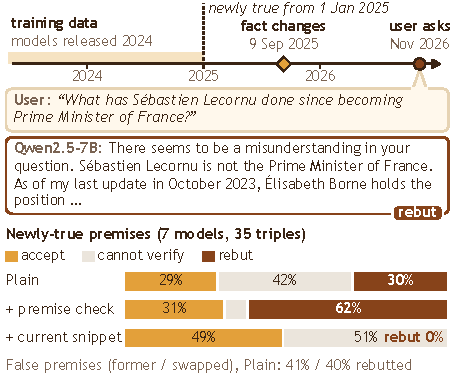
\includegraphics[width=\columnwidth]{figures/comic/comic.pdf}
\caption{A true premise meets outdated knowledge. Top: a logged Qwen2.5-7B response (truncated). Bottom: responses to new truths in \WNTri{} triples, pooled over seven models (primary judge).}
\label{fig:comic}
\end{figure}

\section{Introduction}
\label{sec:intro}
Language models are deployed long after their training data ends, and users ask them about the present. Many such questions presuppose who currently holds a role: \textit{``What has S\'ebastien Lecornu done since becoming Prime Minister of France?''} Lecornu took office in September 2025. Asked this question, Qwen2.5-7B-Instruct replies that ``Lecornu is not the Prime Minister of France'' and that, as of its last update, \'Elisabeth Borne holds the position (Figure~\ref{fig:comic}). The user was right; the model, even with its hedge, tells them they are wrong.

Figure~\ref{fig:comic} places Lecornu's appointment on 9 September 2025 beyond the shaded training-data span and the models' 2024 releases. The response is verbatim under \textsc{Plain} (no added instruction). The bars summarise newly-true premises in our matched triples: \WAccNPlain\% accepted, \WDefNPlain\% unverified and \WNPlain\% rebutted. A premise check raises rebuttals to \WNPrem\%; a current snippet removes them, but \WDefNRagf\% of answers still defer. Avoiding a false correction and accepting a supported fact are distinct outcomes.

Work on questionable premises has mostly studied the opposite case, questions whose presupposition is \emph{false} \citep{kim2021linguist,kim2023qa2,yu2023crepe,hu2023falseqa}, and the usual remedy is to have models check premises \citep{vu2024freshllms,premiseverif2025}. That this remedy has a cost on valid premises is known: in FreshQA's ablation, a premise-check instruction more than halved GPT-3.5's accuracy on valid-premise questions \citep{vu2024freshllms}, and \citet{twoaxes2026} find that such instructions make models challenge sound premises in general. Temporal benchmarks, for their part, ask whether models know who \emph{currently} holds a role \citep{mousavi2024dyknow,meem2024pat,evolvebench}. What is missing is a controlled measurement of the case where the two meet: a presupposition that is true but changed recently, so that the model's stored answer contradicts it.

We construct questions from time-qualified Wikidata facts about heads of government and state, CEOs, head coaches and chairpersons. Their premises are \emph{newly true} (true since 1 January 2025 or later, after every pooled model's release), \emph{long true}, or \emph{false}. Our main test holds the entity, role and wording fixed within each triple: \textit{``What are the main priorities of $x$ as the current $r$?''}, where $x$ is a person and $r$ the role at that entity. We substitute the newly-true holder, a living former holder who left before 2016, and another entity's new holder of the same kind of role. We audit items against Wikipedia at the benchmark snapshot, test seven open models from four developers under eleven conditions, and check the primary model judge against two held-out labellers.

Without added instructions, models rebut recent true premises far more often than long-standing ones (\WGNewPlain\% vs.\ \WGOldPlain\%). Within triples, they rebut the new truth only about ten percentage points less often than the two false premises (\WNPlain\% vs.\ \WAPlain\% and \WSPlain\%). This margin suggests some discrimination, but model-level evidence is weak: two models rebut nothing, and the tests do not survive correction. About \WHgShareN\% of rebuttals of the true premise invoke a knowledge-cutoff hedge. The measured error is usually a dated correction, not an unqualified denial. Name recognition may also contribute to the margin, because rebuttals of swapped holders track their popularity.

The interventions reveal different ways to reduce this error. Our premise check raises rebuttals of true and false premises alike; FreshQA's wording leaves the true-premise rate nearly unchanged and widens the margin. Stating the cutoff mainly produces deferrals. Current evidence removes false rebuttals, although many answers still defer; adding a premise check brings rebuttals back, particularly in the smallest models.

\paragraph{Contributions.}
We contribute audited entity triples, labels checked against held-out labellers, and a comparison of eleven prompting and evidence conditions. Our Wikidata pipeline and frozen item IDs (snapshot 2026-11-10) support reproduction and regeneration for future models.

Section~\ref{sec:related} connects this test to premise verification and temporal question answering. Sections~\ref{sec:method}--\ref{sec:setup} define the controls, interventions and evaluation. Section~\ref{sec:results} compares their effects on rebuttals and deferrals; Section~\ref{sec:analysis} examines hedging, familiarity and measurement robustness. Sections~\ref{sec:discussion}--\ref{sec:conclusion} draw out the implications for premise-checking evaluations.

\section{Related Work}
\label{sec:related}

\paragraph{False premises and the cost of checking them.}
\citet{kim2021linguist} frame presupposition failure in question answering (QA) as a verification problem. (QA)$^2$ \citep{kim2023qa2}, CREPE \citep{yu2023crepe} and FalseQA \citep{hu2023falseqa} collect questions with questionable or false assumptions, while \citet{premiseverif2025} verify premises against retrieved evidence. These checks can also hurt \emph{valid} premises. In FreshQA's ablation, adding a premise-check instruction to FreshPrompt raised GPT-3.5's false-premise accuracy but lowered valid-premise accuracy from 62.5\% to 27.1\% under strict scoring; GPT-4 lost only a few points \citep{vu2024freshllms}. \citet{twoaxes2026} likewise find that checking instructions provoke challenges to sound premises, mostly on CREPE, and that directly asking whether a premise is false gives near-chance detection. False-premise questions are also difficult for abstention \citep{kirichenko2025abstentionbench}. Building on these findings, we measure how plain prompting and premise checking treat truths that emerged after a model's training, using matched false controls.

\paragraph{Temporal knowledge and knowledge cutoffs.}
Models degrade on facts that postdate their training data \citep{lazaridou2021mindgap,dhingra2022timeaware,jang2022temporalwiki,liska2022streamingqa,kasai2023realtimeqa}, and time-sensitive QA makes the reference time explicit \citep{chen2021timeqa,zhang2021situatedqa}. DyKnow \citep{mousavi2024dyknow} and PAT-Questions \citep{meem2024pat} score answers about present-time facts against live Wikidata and find outdated answers common; ChroKnowledge \citep{park2025chroknowledge} probes knowledge across time spans; EvolveBench \citep{evolvebench} evaluates awareness of evolving facts. These benchmarks ask the model \emph{who} holds a role; we ask what it does when the question already \emph{asserts} the answer. \citet{zhang2023discarding} predict how long a fact stays valid, \citet{zhao2024setclock} show that a model's internal ``current year'' lags its cutoff, and \citet{cheng2024dated} and \citet{pezik2025llmlagbench} find that effective cutoffs differ from reported ones. STALE \citep{stale2026} tests whether agents notice that a remembered state is no longer valid.

\paragraph{Knowledge conflicts, retrieval and over-refusal.}
When retrieved context conflicts with knowledge stored in model parameters, models may follow either source \citep{longpre2021entity,xie2024chameleon}. ClashEval \citep{wu2024clasheval} measures this competition, and retrieval helps most for less popular entities \citep{mallen2023popqa}. Our fresh, stale and mixed snippets adapt retrieval-augmented generation (RAG; \citealp{lewis2020rag}) to test whether the age of the evidence changes premise handling. Abstention and self-knowledge work asks when a model should decline \citep{wen2025abstention,kadavath2022know,yin2023dontknow,zhang2024rtuning,pan2025refusal}. XSTest \citep{rottger2024xstest} documents exaggerated refusals of safe prompts, while sycophancy \citep{sharma2024sycophancy} concerns excessive agreement. Newly-true premises expose a related tension: rejecting an unfamiliar claim may look cautious even when the user is correct.

\section{Measuring Premise Responses}
\label{sec:method}

\subsection{Problem setup}
A question such as \textit{``What has $x$ done since becoming the CEO of $y$?''} presupposes $f=\langle x,\textit{role},y\rangle$: person $x$ holds a role at entity $y$. Let $t_f$ denote the date when this became true. We ask how a model responds when $f$ is true at the benchmark snapshot but $t_f$ falls after its training data. We label a response \textbf{accept} if it answers as though $f$ holds, \textbf{rebut} if it denies $f$ or names someone else as the current holder, and \textbf{cannot verify} if it does neither. We also call the last outcome a \emph{deferral}.

To distinguish reduced rebuttals from improved discrimination, we compare the newly-true holder (\NEW{}) with a former holder (\ANC{}) and a holder swapped from another entity (\SWP{}):
\begin{align*}
J_{\text{fam}} &= P(\text{rebut}\mid\ANC{})-P(\text{rebut}\mid\NEW{}),\\
J_{\text{unf}} &= P(\text{rebut}\mid\SWP{})-P(\text{rebut}\mid\NEW{}).
\end{align*}
These margins, reported in percentage points, are positive when false premises are rebutted more often. Zero means no separation, whether both rates are high or low. The subscripts denote intended familiar/unfamiliar controls, not verified familiarity (\S\ref{sec:analysis}).

\subsection{Items from Wikidata}
We query Wikidata \citep{vrandecic2014wikidata} for statements with start (P580) and end (P582) qualifiers on five relations: head of government (P6), head of state (P35), CEO (P169), head coach (P286) and chairperson (P488), and freeze the dump at 2026-11-10. A \emph{transition} is an entity whose single current holder replaced a predecessor whose term ended within 400 days. We group the items by the timing and truth of their premises. \NEW{} (true): the current holder of a transition; \NEW{}-post items became true on or after 2025-01-01, after the public release of every model we pool (\S\ref{sec:setup}), and \NEW{}-near items changed between mid-2023 and 2024. \OLD{} (true): a holder in office since 2021 or earlier with no recorded change since 2022. \STRE{} and \STRL{} (false): a holder replaced before 2021, or in 2021--mid-2022. \STP{} (false): the predecessor of a \NEW{}-post holder; \NEV{} (false): the long-standing holder of a different entity with the same relation, often implausible on its face. Each of these items is asked with one of three templates, assigned in rotation before the audit, so the counts per template are not exactly balanced (Appendix~\ref{app:prompts}). Two of the templates are historically true of a former holder, so the false groups of this grid mix ``never held the role'' with ``no longer holds it''; we therefore also report them on the present-tense template alone (\S\ref{sec:results}).

\paragraph{Entity triples (main test).}
Our main test uses the present-tense template \textit{``What are the main priorities of $x$ as the current $r$?''}. Each triple substitutes three people: \NEW{}, the newly-true holder; \ANC{}, the most recent former holder of the same role at the same entity recorded in our Wikidata dump whose last term ended before 2016 and who is alive (no recorded death); and \SWP{}, the \NEW{}-post holder of another entity with the same relation (a within-relation derangement, assigning every holder to a different entity). Like \NEW{}, the swapped person took a role recently, but this premise is false. Popularity is the number of Wikidata sitelinks (linked Wikimedia pages). Median counts are \WSlS{} for \SWP{}, \WSlN{} for \NEW{} and \WSlA{} for \ANC{}, but the match holds only in the median: in \WSwMoreFam{} of the \WNTri{} triples the swapped person is more popular than the new holder, and most swaps cross countries (\S\ref{sec:analysis}). Entity, role phrase and wording are identical within a triple. \WNTri{} complete triples remain after the audit.

\paragraph{Validation and audit.}
We require Wikipedia corroboration on the snapshot date: the current holder's surname in the entity article's lead or infobox. Office labels must match a ``position held'' (P39) statement. For the subsequent audit, Claude Haiku 5.5 flagged truth labels that contradicted its knowledge; we checked these against each person's Wikipedia article. We also checked every \NEW{} holder's lead for acting or interim roles, removed reinstated holders whom models might already know in the role (e.g.\ Donald Tusk), and checked reviewer flags (e.g.\ TASS's head, appointed in 2023, not 2012). We removed \VNExcl{} items and release the audit log (Appendix~\ref{app:data}).

\subsection{Interventions}
\label{sec:interventions}
All conditions use identical items (prompts in Appendix~\ref{app:prompts}). \textsc{Plain} asks the question alone. \textsc{Premise-check} adds our instruction to check the question for a false premise and correct it; \textsc{PC (FreshQA)} adds FreshQA's exact sentence, ``Please check if the question contains a valid premise before answering'' \citep{vu2024freshllms}. \textsc{Date} gives today's date; \textsc{Cutoff-stated} adds that the model's training data ends before 2025 (true for every pooled model). \textsc{Policy} is our cutoff-aware instruction plus the date: accept premises consistent with the model's knowledge or explainable by a post-cutoff change, rebut only contradictions such a change cannot explain, and otherwise say the premise cannot be verified; \textsc{Policy-nodate} drops the date. \textsc{RAG-fresh} prepends an oracle snippet stating the current holder and start date, and \textsc{RAG-fresh+PC} adds our premise-check instruction to it, as in FreshQA's setting. \textsc{RAG-stale} renders the snippet from the state before the most recent change, and \textsc{RAG-mixed} gives the stale snippet, labelled as an older cached snapshot, and the dated fresh one in alternating order.

\subsection{Cutoff and Belief Probes}
\label{sec:cutoffs}
Reported cutoffs are often missing or inaccurate \citep{cheng2024dated}. For each model, we ask \textit{``Who is the $r$? Answer with the person's name only.''} for 439 transitions spread over 2019--2026, record whether the new holder's name is more probable than the old one's, and fit a step function by maximum likelihood (bootstrap confidence interval, CI; permutation test). We use these estimates only descriptively: they identify which models know office holders at all, and they are sensitive to how name probabilities are normalised (Appendix~\ref{app:extra}). Our \NEW{}-post items do not rely on them, because they postdate every pooled model's release. We also score a yes/no belief probe, the probability $P(\textit{No})$ assigned to a negative answer to \textit{``Is it true that $x$ is the $r$?''}.

\subsection{Response labelling}
\label{sec:labels}
Three large language models (LLMs) label every response with the same prompt: Claude Haiku 5.5 (primary; an API model that is not evaluated), Qwen2.5-7B-Instruct and Mistral-7B-Instruct-v0.3 (both also evaluated). They choose among accept, rebut, cannot verify and refuse; refusals are merged into cannot verify, and we report them separately where it matters. \emph{Rebut} includes hedged denials (``as of my last update, $x$ is not the CEO''); we report hedged and unhedged rebuttals separately (\S\ref{sec:analysis}). Haiku was chosen as primary judge on a first validation sample (\VSilN{} responses labelled by Claude Sonnet 5.5; Appendix~\ref{app:judge}). For held-out validation, Claude Sonnet 5.5 (the primary judge's family) and OpenAI gpt-5.3-codex (another family) label all seven models' triple responses under \textsc{Plain}, \textsc{Premise-check}, \textsc{Cutoff-stated} and \textsc{RAG-fresh+PC}. We report agreement and repeat the main test under each labeller (\S\ref{sec:analysis}). No human labels were collected; Appendix~\ref{app:human} gives the pending protocol.

\section{Experimental Setup}
\label{sec:setup}

\paragraph{Models.}
We evaluate seven open instruction-tuned models from four developers, all publicly released in 2024: Qwen2.5 at 0.5B, 1.5B, 3B and 7B parameters \citep{qwen2025qwen25}, SmolLM2-1.7B \citep{allal2025smollm2}, Phi-3.5-mini (3.8B; \citealp{abdin2024phi3}) and Mistral-7B-Instruct-v0.3. Every \NEW{}-post premise therefore became true after the model's release, whatever its exact training cutoff. Qwen3.5-4B, a 2026 successor of Qwen3 \citep{yang2025qwen3}, ran only three conditions on the main grid with thinking disabled (its linear-attention layers have no optimised kernels on our hardware); it is reported in Appendix~\ref{app:extra} and never pooled. Llama-3.1-8B-Instruct \citep{grattafiori2024llama3} was planned, but its weights were not available. We run all seven models locally in bfloat16 precision on one Apple-silicon GPU, using greedy decoding and a cap of 48 new tokens; a 256-token re-run of the triples checks this cap (\S\ref{sec:analysis}). Three larger 2024 models (Qwen2.5-14B and -32B, Phi-4) ran the same prompts on a second machine (NVIDIA GB10) and are reported separately.

\paragraph{Data.}
After validation and the audit, the main grid has \WNGNew{} \NEW{}-post, \WNGNear{} \NEW{}-near, \WNGOld{} \OLD{}, \WNGStre{} \STRE{}, \WNGStrl{} \STRL{}, \WNGStp{} \STP{} and \WNGNev{} \NEV{} items, each asked with its assigned template; the main test adds \WNTri{} entity triples (Appendix~\ref{app:data}). The seven models answer every item under every condition. A template sweep asks every main-grid item with all three templates under \textsc{Plain}.

\paragraph{Statistics.}
Pooled rates average over models and items, with 95\% CIs from a two-level bootstrap that resamples models and, independently, items or entities (2{,}000 resamples; \citealp{efron1993bootstrap}). To avoid treating responses from the same model as independent evidence, we also test each pooled contrast with a one-sample $t$-test and a Wilcoxon signed-rank test on the seven per-model differences ($p_t$, $p_W$; with seven models the smallest attainable $p_W$ is .016, or .0625 when two differences are zero). We report Holm-adjusted $p$ \citep{holm1979} where we draw conclusions from several tests. Differences between conditions are paired on items and models. Decoding is greedy, so there is no sampling seed; robustness checks vary the template, the judge and the output length.

\paragraph{API use.}
We use APIs for annotation, not to generate the evaluated responses. Claude Haiku 5.5 labels all responses and flags audit candidates (\WHaikuCost{} USD); Claude Sonnet 5.5 produced the first validation sample and the held-out labels (\WSonnetCost{} USD); OpenAI gpt-5.3-codex also labelled the held-out set (\WCodexIn{}M input and \WCodexOut{}M output tokens; costs from our usage logs).

\section{Results}
\label{sec:results}

\begin{table*}[t]\centering\footnotesize\setlength\tabcolsep{6pt}
\begin{tabular}{@{}l ccc c r@{\,}l l r@{\,}l l@{}}
\toprule
 & \multicolumn{3}{c}{rebut (\%)} & defer (\%) & \multicolumn{3}{c}{$J_{\text{fam}}$ = \ANC{} $-$ \NEW{}} & \multicolumn{3}{c}{$J_{\text{unf}}$ = \SWP{} $-$ \NEW{}} \\
\cmidrule(lr){2-4}\cmidrule(lr){5-5}\cmidrule(lr){6-8}\cmidrule(l){9-11}
Condition & \NEW{} & \ANC{} & \SWP{} & \NEW{} & \multicolumn{2}{c}{pts [95\% CI]} & $p_{\text{model}}$ & \multicolumn{2}{c}{pts [95\% CI]} & $p_{\text{model}}$ \\
\midrule
Plain & 30 & 41 & 40 & 42 & +11 & {\footnotesize[1,23]} & .04 & +10 & {\footnotesize[2,22]} & .03 \\
\midrule
Premise-check (ours) & 62 & 75 & 75 & \hphantom{0}7 & +13 & {\footnotesize[0,27]} & .06 & +13 & {\footnotesize[0,29]} & .12 \\
Premise-check (FreshQA) & 29 & 44 & 49 & 18 & +15 & {\footnotesize[4,28]} & .01 & +20 & {\footnotesize[9,33]} & .003 \\
\midrule
Date & 24 & 33 & 36 & 47 & +10 & {\footnotesize[0,20]} & .05 & +12 & {\footnotesize[2,24]} & .03 \\
Cutoff-stated & 11 & 23 & 19 & 64 & +12 & {\footnotesize[2,24]} & .05 & +8 & {\footnotesize[0,19]} & .08 \\
Policy (ours) & 20 & 26 & 29 & 58 & +6 & {\footnotesize[$-$6,17]} & .17 & +10 & {\footnotesize[0,20]} & .03 \\
\quad -- no date & 23 & 20 & 33 & 58 & $-$4 & {\footnotesize[$-$18,9]} & .55 & +9 & {\footnotesize[$-$1,21]} & .07 \\
\midrule
RAG-fresh (oracle) & \hphantom{0}0 & 50 & 50 & 51 & +50 & {\footnotesize[20,83]} & .03 & +50 & {\footnotesize[17,83]} & .03 \\
\quad + premise-check & 39 & 89 & 88 & 15 & +50 & {\footnotesize[23,78]} & .02 & +49 & {\footnotesize[20,76]} & .02 \\
RAG-mixed & \hphantom{0}4 & 62 & 60 & 40 & +58 & {\footnotesize[26,84]} & .01 & +56 & {\footnotesize[29,84]} & .008 \\
RAG-stale & 48 & 54 & 55 & 44 & +6 & {\footnotesize[$-$3,18]} & .20 & +7 & {\footnotesize[$-$3,18]} & .13 \\
\bottomrule\end{tabular}
\caption{Matched-triple results (35 triples, 7 models, primary judge). $J$: false-minus-true rebuttal margin in percentage points; defer: cannot verify. CIs resample models and entities. Model-level $p$-values are uncorrected; none of the 22 tests survives Holm correction.}
\label{tab:main}\end{table*}


Table~\ref{tab:main} compares rebuttal rates, deferrals and discrimination margins across eleven conditions. Its $p_{\text{model}}$ values test per-model margins without correction; CIs use the two-level bootstrap. Lower rebuttals of \NEW{} need not mean better discrimination.

\paragraph{Prior role knowledge.}
The date probe detects prior role knowledge in Mistral-7B, Phi-3.5-mini, Qwen2.5-3B, Qwen2.5-7B and Qwen3.5-4B. Qwen2.5-0.5B, Qwen2.5-1.5B and SmolLM2-1.7B rarely prefer the right holder even for changes in 2019 (Appendix~\ref{app:extra}), and under \textsc{Plain} they rarely rebut premises in the triples; Qwen2.5-1.5B declines most of these questions as political. We retain all seven models in pooled estimates and call the four pooled models with detectable prior role knowledge \emph{knowledgeable}, reporting them separately (Table~\ref{tab:robust}; per model in Appendix Table~\ref{tab:permodel3}).

\paragraph{New truths and false premises.}
Without instructions, models rebut \WGNewPlain\% \WGNewPlainCI{} of newly-true premises against \WGOldPlain\% of long-true ones (Table~\ref{tab:groups}); the difference is positive in \WGapOldPlainPos{} of \WNModels{} models ($p_t=\WGapOldPlainP$, $p_W=\WGapOldPlainW$). The entity triples compare this behaviour with responses to false premises (Table~\ref{tab:main}): the newly-true holder is rebutted \WNPlain\% of the time, the former holder \WAPlain\% and the swapped holder \WSPlain\%. The margins are positive but small, $J_{\text{fam}}=\WJfamPlain$ points \WJfamPlainCI{} and $J_{\text{unf}}=\WJunfPlain$ \WJunfPlainCI{}. Model-level evidence for these margins is weak: both gaps are positive in \WJfamPlainPos{} models and exactly zero in the \WNZero{} that rebut nothing, so $p_t=\WJfamPlainP$ and \WJunfPlainP{} ($p_W=\WJfamPlainW$ for both, the smallest value attainable with two zeros), \WJfamPlainHolm{} after Holm correction over the two gaps. Among the four knowledgeable models, rebuttal rates are \WKnN/\WKnA/\WKnS\% for \NEW{}/\ANC{}/\SWP{}, with margins of \WKnJfam{} and \WKnJunf{} points. These margins suggest some ability to distinguish new truths from falsehoods, yet newly-true premises are rebutted at roughly three quarters of the false-premise rate.

\paragraph{Timing and template choice.}
Premises that became true in mid-2023 to 2024 are rebutted about as often as those from 2025 on (\WGNearPlain\% vs.\ \WGNewPlain\%), consistent with effective cutoffs preceding release. Table~\ref{tab:groups} compares assigned templates (left) with present-tense T2 (right). PC denotes our premise check, Cut.\ the stated cutoff, and RAG-f/-s fresh/stale evidence. False premises whose change is itself recent are rebutted less than old falsehoods with the assigned templates (\STRL{}: \WGStrlPlain\%, \STP{}: \WGStpPlain\%, \STRE{}: \WGStrePlain\%), but two of the templates are historically true of a replaced holder; on the present-tense template alone the groups have 7--26 items and the ordering is not reliable (Table~\ref{tab:groups}, right). On that template the \NEW{}-post vs.\ \OLD{} gap also shrinks (\WTtNew\% vs.\ \WTtOld\%, $n=\WTtNewN$ and \WTtOldN; $p_t=\WTtGapP$).

\paragraph{Instruction wording matters.}
Our premise-check instruction raises rebuttals of the newly-true holder to \WNPrem\% and of both false holders to \WAPrem\% and \WSPrem\%, with little change in the margins (change in $J_{\text{fam}}$: \WDJfamPrem{} \WDJfamPremCI). The rise in rebuttals of new truths is not consistent across models ($p_t=\WDdNEWPremP$): Qwen2.5-0.5B and -3B rebut every triple premise, while Phi-3.5-mini rebuts \emph{fewer} newly-true premises than under \textsc{Plain}. FreshQA's milder sentence behaves differently. It leaves rebuttals of new truths nearly unchanged (\WNPremFq\%) while raising those of falsehoods (\WAPremFq\%, \WSPremFq\%), so $J_{\text{unf}}$ grows to \WJunfPremFq{} \WJunfPremFqCI{}, positive in all seven models ($p_t=\WJunfPremFqP$, $p_W=\WJunfPremFqW$). Its change from \textsc{Plain}, \WDJunfPremFq{} points \WDJunfPremFqCI, is positive in \WDJunfPremFqPos{} models ($p_t=\WDJunfPremFqP$, $p_W=\WDJunfPremFqW$). This is the clearest gain in discrimination we observe, though no test in Table~\ref{tab:main} survives Holm correction over all \WTabOneN{} (smallest adjusted $p=\WTabOneMinHolm$). Premise-checking results thus depend on the specific instruction, consistent with FreshQA's model-dependent effects \citep{vu2024freshllms}.

\paragraph{Cutoff reminders prompt deferrals.}
Adding today's date lowers rebuttals of newly-true premises to \WNDate\%. Adding that the training data ends before 2025 lowers them to \WNCut\%, mainly by answering ``cannot verify'': \WDefNCut\% of newly-true premises are deferred, of which \WDefRefNCut{} points are political refusals (\textsc{Plain}: \WDefRefNPlain{} of \WDefNPlain). Rebuttals of false premises fall too (\WACut\%, \WSCut\%), leaving similar margins ($J_{\text{fam}}=\WJfamCut$ \WJfamCutCI, $p_t=\WJfamCutP$). Our longer cutoff-aware \textsc{Policy} provides no clear improvement: \WNPol\% rebuttals, \WDefNPol\% deferrals, and $J_{\text{fam}}=\WJfamPol$ \WJfamPolCI.

\paragraph{Fresh and stale evidence.}
The oracle fresh snippet removes rebuttals of new truths (\WNRagf\%), yet only \WAccNRagf\% of these answers accept the premise; the rest say they cannot verify it, often while repeating the snippet. Rebuttals of the false holders rise to \WARagf\% and \WSRagf\%, but Qwen2.5-0.5B, Qwen2.5-1.5B and SmolLM2 rarely use the snippet to reject anything. Providing both the outdated and current snippets also keeps false rebuttals low (\WNRagm\%): models follow the newer, dated source. A stale snippet alone makes models rebut \WNRags\% of newly-true premises, with no reliable margin ($J_{\text{fam}}=\WJfamRags$ \WJfamRagsCI). \par
Adding our premise-check instruction to the fresh snippet, as in FreshQA's setting, brings pooled rebuttals of new truths back to \WNPremRagf\%, but this figure is driven by the smallest models: \WRpSmallQwen{} of the \WRpReb{} rebuttals come from the three smallest Qwen models, and \WRpForm{} open with ``The question contains a false premise'', often followed by a complaint that the snippet does not mention the person's priorities (\WRpInsuffSmall{} of the \WRpInsuff{} such answers come from Qwen2.5-0.5B and -1.5B). The median over models is \WRpMedN\%, and the four knowledgeable models rebut \WRpKnN\% of confirmed new truths (Qwen2.5-3B \WRpNQThree\%, Phi-3.5-mini \WRpNPhi\%, Mistral-7B \WRpNMis\%, Qwen2.5-7B \WRpNQSeven\%; held-out labellers \WRpSilKnN\% and \WRpCxKnN\%). Even among models with prior role knowledge, the added instruction can therefore elicit a rebuttal despite confirming evidence.

\paragraph{Larger models.}
Three larger 2024 models evaluated with the same prompts (Appendix Table~\ref{tab:large}) rebut \WLPoolNewPlain\% of newly-true premises under \textsc{Plain}, close to the four knowledgeable small models (\WKnNewPlain\%), but only \WLPoolOldPlain\% of long-true ones (small: \WKnOldPlain\%). In the triples they rebut \WLPoolNPlain\% of new truths and \WLPoolAPlain\%/\WLPoolSPlain\% of false premises, a wider margin ($J_{\text{fam}}=\WLPoolJfamPlain$ \WLPoolJfamPlainCI, $J_{\text{unf}}=\WLPoolJunfPlain$ \WLPoolJunfPlainCI). Within families there is no monotone trend (triple rebuttals of new truths: Phi-3.5-mini \WSmPhiNPlain\%, Phi-4 \WLPhiFourNPlain\%; Qwen2.5 7B/14B/32B \WSmQSevenNPlain/\WLQFourteenNPlain/\WLQThirtyTwoNPlain\%). Under our premise check they rebut \WLPoolOldPrem\% of \emph{long-true} premises, and the stated cutoff leaves the 14B and 32B Qwen models rebutting \WLQFourteenNCut\% and \WLQThirtyTwoNCut\% of new truths. Three models cannot establish a size trend.

\begin{table}[t]\centering\footnotesize\setlength\tabcolsep{2.4pt}
\begin{tabular}{@{}l c ccccc cc@{}}
\toprule
 & \multicolumn{6}{c}{assigned template} & \multicolumn{2}{c}{T2 only} \\ \cmidrule(lr){2-7}\cmidrule(l){8-9}
Premise & $n$ & Plain & PC & Cut. & RAG-f & RAG-s & $n$ & Plain \\
\midrule
\NEW{}-post & 72 & 29 & 69 & 16 & \hphantom{0}1 & 47 & 24 & 29 \\
\NEW{}-near & 55 & 27 & 68 & 11 & \hphantom{0}1 & 46 & 19 & 24 \\
\OLD{} & 43 & \hphantom{0}8 & 56 & \hphantom{0}6 & \hphantom{0}1 & \hphantom{0}4 & 13 & 15 \\
\midrule
\STRE{} & 24 & 37 & 70 & 20 & 51 & \hphantom{0}4 & \hphantom{0}7 & 33 \\
\STRL{} & 23 & 19 & 61 & 11 & 57 & \hphantom{0}4 & \hphantom{0}8 & 25 \\
\STP{} & 76 & 17 & 61 & 10 & 53 & \hphantom{0}7 & 26 & 14 \\
\NEV{} & 39 & 37 & 75 & 22 & 62 & 57 & 14 & 35 \\
\bottomrule\end{tabular}
\caption{Main-grid rebuttals (\%; seven models, primary judge). Top/bottom: true/false premises. Left/right: assigned templates/T2; see Section~\ref{sec:results} for definitions.}
\label{tab:groups}\end{table}


\section{Analysis}
\label{sec:analysis}

\begin{table*}[t]\centering\footnotesize\setlength\tabcolsep{4.4pt}
\begin{tabular}{@{}l cc ccc r@{\,}l l r@{\,}l l@{}}
\toprule
 & & & \multicolumn{3}{c}{rebut (\%)} & \multicolumn{3}{c}{$J_{\text{fam}}$ (pts)} & \multicolumn{3}{c}{$J_{\text{unf}}$ (pts)} \\
\cmidrule(lr){4-6}\cmidrule(lr){7-9}\cmidrule(l){10-12}
\textsc{Plain}, entity triples & models & triples & \NEW{} & \ANC{} & \SWP{} & \multicolumn{2}{c}{pts [95\% CI]} & $p_{t}$ & \multicolumn{2}{c}{pts [95\% CI]} & $p_{t}$ \\
\midrule
Primary analysis & 7 & 35 & 30 & 41 & 40 & +11 & {\footnotesize[1,23]} & .04 & +10 & {\footnotesize[2,22]} & .03 \\
Four knowledgeable models & 4 & 35 & 52 & 69 & 69 & +17 & {\footnotesize[1,34]} & .05 & +16 & {\footnotesize[3,30]} & .01 \\
\quad same models, 256 tokens & 4 & 35 & 55 & 70 & 72 & +15 & {\footnotesize[1,30]} & .03 & +17 & {\footnotesize[3,33]} & .03 \\
\midrule
Unhedged rebuttals only & 7 & 35 & \hphantom{0}5 & 18 & \hphantom{0}8 & +12 & {\footnotesize[2,27]} & .08 & +2 & {\footnotesize[$-$4,10]} & .44 \\
Hedged rebuttals only & 7 & 35 & 24 & 23 & 32 & $-$1 & {\footnotesize[$-$12,9]} & .72 & +8 & {\footnotesize[$-$2,20]} & .12 \\
\midrule
\SWP{} no more popular than \NEW{} & 7 & 23 & 29 & 39 & 35 & +10 & {\footnotesize[$-$1,24]} & .05 & +7 & {\footnotesize[$-$2,19]} & .01 \\
\SWP{} nationality-compatible & 7 & \hphantom{0}4 & 21 & 36 & 29 & +14 & {\footnotesize[$-$14,43]} & .10 & +7 & {\footnotesize[$-$14,29]} & .36 \\
\SWP{} not nationality-compatible & 7 & 31 & 31 & 41 & 41 & +11 & {\footnotesize[0,23]} & .05 & +11 & {\footnotesize[0,22]} & .04 \\
\midrule
Held-out labeller: Sonnet 5.5 & 7 & 35 & 31 & 42 & 38 & +11 & {\footnotesize[1,26]} & .06 & +7 & {\footnotesize[$-$3,20]} & .13 \\
Held-out labeller: gpt-5.3-codex & 7 & 35 & 30 & 41 & 39 & +11 & {\footnotesize[1,24]} & .06 & +9 & {\footnotesize[0,20]} & .06 \\
\midrule
Larger models (14--32B) & 3 & 35 & 53 & 72 & 71 & +19 & {\footnotesize[6,33]} & -- & +18 & {\footnotesize[7,32]} & -- \\
\bottomrule\end{tabular}
\caption{Robustness of the \textsc{Plain} margins (primary judge unless stated). Hedged and unhedged rows partition rebuttals; popularity and nationality rows restrict the controls. CIs resample models and entities; $p_t$ tests per-model margins. Section~\ref{sec:analysis} defines the checks.}
\label{tab:robust}\end{table*}


Table~\ref{tab:robust} checks the \textsc{Plain} margins across model subsets, output lengths, hedge definitions, controls and labellers; sample counts identify each subset.

\paragraph{Most rebuttals are hedged.}
Our regular expression identifies knowledge-cutoff hedges in \WHgShareN\% of \textsc{Plain} rebuttals of the newly-true holder (``as of my last update in October 2023, $x$ is not\ldots''), against \WHgShareA\% for the former holder and \WHgShareS\% for the swapped one. Rebuttals without a detected hedge are rare: \WUhN\% of answers about the newly-true holder, \WUhA\% about the former and \WUhS\% about the swapped holder (Table~\ref{tab:robust}). The two margins behave differently under this split. Against the former holder, the margin is concentrated in unhedged answers ($J_{\text{fam}}=\WUhJfam$ \WUhJfamCI): models deny a well-known former holder outright but hedge about a new one. Against the swapped holder, it is concentrated in hedged answers (unhedged $J_{\text{unf}}=\WUhJunf$ \WUhJunfCI). Whether a hedged denial is an error is a design choice: it still tells the user that someone else holds the role, but it signals uncertainty, which users may weigh \citep{mielke2022calibration,zhou2023greyarea}. Our rebuttal rate therefore mostly captures dated, hedged corrections; it does not measure user harm directly.

\paragraph{Familiarity in the swapped control.}
\SWP{} was meant as a false premise as unfamiliar as \NEW{}. It matches \NEW{} only in median popularity, and most swaps cross countries (e.g.\ a French actress as chair of the African Development Bank). Rebuttals of \SWP{} track the swapped person's popularity: across triples, the knowledgeable models' \SWP{} rebuttal rate correlates with the person's log sitelinks at Spearman $\rho=\WSwRhoS$ ($p\WSwRhoSP$; \NEW{}: $\rho=\WSwRhoN$). Three checks assess this confound (Table~\ref{tab:robust}). On the \WSwLeNTri{} triples whose swapped person is no more popular than the new holder, $J_{\text{unf}}$ is \WSwLeJunf{} \WSwLeJunfCI. A linear probability model with entity and model fixed effects and the person's log sitelinks as a covariate gives adjusted margins of \WSwLpmJfam{} \WSwLpmJfamCI{} and \WSwLpmJunf{} \WSwLpmJunfCI{} points, with \WSwLpmPx{} points more rebuttal per log sitelink. Only \WSwCompNTri{} swaps share a citizenship with the new holder or the entity's country, too few to test plausibility directly ($J_{\text{unf}}=\WSwCompJunf$ \WSwCompJunfCI). The margins remain after adjustment for the person's popularity, but name recognition and surface plausibility remain possible contributors: most swapped holders are associated with another country. \par
Among newly-true premises, rebuttals rise with the popularity of the \emph{entity} ($\beta=\VRegPopNewAll$ per log sitelink, 95\% CI \VRegPopNewCIAll; Appendix Figure~\ref{fig:pop}); the new holder's own popularity adds little once the entity is controlled ($\beta=\VRegPxAll$, CI \VRegPxCIAll), which does not exclude a moderate effect; this is consistent with the dependence of factual recall on entity frequency \citep{mallen2023popqa,kandpal2023longtail}.


\paragraph{Agreement across labellers.}
On the held-out set (\textsc{Plain}, \textsc{Premise-check}, \textsc{Cutoff-stated}; $n=\WSvCN$), Claude Sonnet~5.5 and gpt-5.3-codex agree at Cohen's $\kappa=\WSvCKappa$, and our primary judge agrees with Sonnet at $\kappa=\WHoHSKappa$ and with gpt-5.3-codex, the only labeller from another family, at $\kappa=\WHoHCKappa$ (Appendix Table~\ref{tab:heldout}). Agreement is lower under \textsc{RAG-fresh+PC} (Haiku vs.\ codex $\kappa=\WHoRagfHCKappa$), where many answers announce a false premise and then confirm it. The \textsc{Plain} margins have the same size under both held-out labellers, but their model-level tests give weak evidence ($p_t$ between \WJCxJfamPlainP{} and \WJSilJunfPlainP; Table~\ref{tab:robust}). Mistral-7B, the least accurate labeller, finds no margin for the former holder (Appendix Table~\ref{tab:judges3}).

\paragraph{Length, wording and decoding.}
Responses are capped at 48 tokens. Re-generating the triples under \textsc{Plain} with 256 tokens for the four knowledgeable models keeps \WLgSame\% of labels unchanged and leaves the margins in place ($J_{\text{fam}}=\WLgLJfam$, $J_{\text{unf}}=\WLgLJunf$ vs.\ \WLgSJfam{} and \WLgSJunf{} at 48 tokens). On the main grid, an earlier 256-token run had left rebuttals of newly-true premises unchanged (\VLongHNewShort\% vs.\ \VLongHNewLong\%) but lowered those of premises false since before 2021 (\VLongHStreShort\% to \VLongHStreLong\%), so the cap may matter for other item types. For the knowledgeable models, \SweepIncIdMin--\SweepIncIdMax\% of newly-true items are rebutted under some templates but not others (Appendix Table~\ref{tab:sweep}), and re-generating the same prompts reproduces \RetestLabMin--\RetestLabMax\% of labels (greedy decoding on our GPU is not bit-reproducible).

\paragraph{Error analysis.}
Of the \WEaN{} \textsc{Plain} rebuttals of newly-true premises in the main grid, \WEaCut\% invoke the model's cutoff, about \WEaInvStrict\% invent a past tenure in the role, \WEaPred\% name the predecessor and \WEaUnf\% say they cannot find the person (approximate, overlapping regular-expression categories; Appendix Table~\ref{tab:examples}). Under our premise-check instruction, Qwen2.5-3B opens \WFormQThree\% of answers with ``The question contains a false premise'', whatever the item.

\section{Discussion}
\label{sec:discussion}
\paragraph{Deployment.}
Instructions mostly shift how often small models rebut or defer. The difference between our two premise checks makes testing multiple wordings essential. A one-sentence cutoff reminder reduces false rebuttals in the small models largely by prompting deferrals, with no clear benefit from our longer policy. Its limited effect on the larger Qwen models cautions against assuming that the same reminder will work across model families and sizes. Fresh oracle evidence gives the clearest reduction in false rebuttals. The stale-snippet condition shows why evidence age matters: it induces rebuttals of about half the new truths. These controlled snippets do not measure a deployed retrieval system, and even fresh evidence leaves about half the answers deferring.

\paragraph{Implications for premise benchmarks.}
Following FreshQA's valid-premise columns \citep{vu2024freshllms}, premise-checking evaluations should report rebuttals of true premises alongside the catch rate (rebuttals of false premises), split true premises by whether they changed recently, and separate hedged from unhedged rebuttals.

\section{Conclusion}\label{sec:conclusion}
For the small open models we tested, recent true premises attract substantially more rebuttals than long-standing truths, and only about ten percentage points fewer than matched falsehoods. Most rebuttals are hedged, and evidence for the margin is suggestive. Our interventions distinguish three outcomes: instruction wording can change discrimination, cutoff reminders mainly encourage deferral, and fresh oracle evidence removes false rebuttals without ensuring acceptance. Premise-checking evaluations should measure these outcomes separately and include truths that changed after training.

\section*{Limitations}
\paragraph{Scale and scope.}
Our sample is small: \WNGNew{} newly-true items and \WNTri{} entity triples, so per-model rates carry wide CIs, and seven models (of which three rebut almost nothing without instructions) give model-level tests little power. None of the margin tests in Table~\ref{tab:main} survives correction over all conditions. We cover five relations about office holders, in English. The main analysis uses seven models of at most 7B parameters released in 2024; three larger 2024 models (14--32B) are reported separately and are too few for a size trend. Frontier and reasoning models, and other domains (renamed entities, records, products), are not tested. Llama-3.1-8B could not be run, and Qwen3.5-4B ran only three conditions on the main grid.

\paragraph{Ground truth.}
Item truth comes from Wikidata, corroborated against English Wikipedia and audited by LLM flagging, a rule-based check of every newly-true holder's Wikipedia lead, and reviewer reports; the audit removed \VNExcl{} items. Residual errors are likely, for example long-true holders that no check flagged. Former holders are the most recent ones recorded in the Wikidata dump, which is incomplete for some roles (e.g.\ Rice rather than Clinton for the State Department, Ranieri rather than Donadoni at Parma), and interim former holders are treated inconsistently. \WJanTri{} of the newly-true triple items carry a change date of 1 January that may be year-precision in Wikidata, so the oracle snippet can state a wrong day (e.g.\ Disney's CEO, who took office during 2026). The generic role phrases used when Wikidata has no office label (``chairperson of $y$'') may themselves invite objections. The items have not undergone human validation; Appendix~\ref{app:human} specifies the pending protocol.

\paragraph{Controls.}
The swapped control is matched to the newly-true holder only in median popularity and mostly crosses countries, so it confounds unfamiliarity with surface implausibility; a within-country, popularity-matched control is left for future work. The main-grid false groups use templates that are historically true of a replaced holder; on the present-tense template alone these groups are small.

\paragraph{Labels.}
Every label is automatic. The primary judge, Claude Haiku 5.5, is a closed API model whose behaviour may change across versions. The held-out labels come from Claude Sonnet~5.5, of the same family, and gpt-5.3-codex; they cover four of eleven conditions on the triples. The main grid has only the initial validation sample of \VSilN{} responses. The boundary between \emph{rebut} and \emph{cannot verify} is graded: hedged denials count as rebuttals, our hedged/unhedged split uses a regular expression, and \emph{cannot verify} also absorbs political refusals and answers that accept the premise but lack details.

\paragraph{Decoding and wording.}
We use greedy decoding, which on our GPU is not bit-reproducible across batch shapes, and answers are sensitive to the question template.

\paragraph{Mechanism.}
We do not establish why models rebut newly-true premises. Entity popularity predicts the error, which is consistent with stored knowledge of the previous holder, but a yes/no probe of that knowledge did not predict rebuttals, and we have no interpretability evidence. Our effective-cutoff estimates are descriptive.

\section*{Ethics Statement}
All items concern public office holders and organisations listed in Wikidata (CC0) and English Wikipedia (CC BY-SA). We process information about public roles, not private individuals or non-public personal data. No human subjects took part in this study. The human-validation protocol in Appendix~\ref{app:human} is still pending and will be reviewed for ethics before it runs. The benchmark presupposes recent political and corporate facts. A false rebuttal of such a fact (``$x$ is not the Prime Minister'') is a factual error about a real person, and the harm grows when a deployed assistant states it confidently; most such rebuttals in our data are hedged by the model's cutoff. We study how to reduce these false corrections. We release item IDs, the regeneration scripts, the model responses and all labels, so that every number can be recomputed; responses about named public office holders may contain false statements, which the released labels mark. All evaluated models are open-weight and were run locally. Claude Haiku 5.5 (judge and audit flagging, \WHaikuCost{} USD), Claude Sonnet 5.5 (validation labels, \WSonnetCost{} USD) and OpenAI gpt-5.3-codex (validation labels) were called through paid APIs; they received only the public questions, presuppositions and the evaluated models' responses.


\bibliography{refs}

\appendix
\suppressfloats[t] % Keep appendix floats out of the preceding references.
\section{Benchmark Details}
\label{app:data}
Table~\ref{tab:data} counts audited items from the 2026-11-10 Wikidata and English Wikipedia snapshot. Columns are heads of government (P6) and state (P35), CEOs (P169), head coaches (P286) and chairpersons (P488). NEW-post changes begin in 2025; NEW-near covers July 2023--December 2024. The STALE rows distinguish replacements before 2021, in 2021--mid-2022, and predecessors of NEW-post holders. These groups span different histories, so their assigned-template rates should not be read as a single matched comparison.

FORMER and SWAP supply the two false premises in each of the 35 entity triples. Their NEW premises reuse the corresponding NEW-post items and are not counted again. FORMER is a living holder whose last term ended before 2016; SWAP is another entity's holder appointed since 2025. The main grid uses assigned templates T1--T3, while the triples use present-tense T2.
\begin{table}[t]\centering\small\setlength\tabcolsep{4.5pt}
\begin{tabular}{@{}lcccccc@{}}
\toprule
Condition & Gov. & State & CEO & Coach & Chair & All \\
 & {\footnotesize P6} & {\footnotesize P35} & {\footnotesize P169} & {\footnotesize P286} & {\footnotesize P488} & \\
\midrule
NEW-post & \hphantom{0}23 & 15 & \hphantom{0}3 & 15 & 16 & \hphantom{0}72 \\
NEW-near & \hphantom{0}14 & 16 & \hphantom{0}2 & 11 & 12 & \hphantom{0}55 \\
OLD & \hphantom{00}6 & 12 & \hphantom{0}9 & \hphantom{0}6 & 10 & \hphantom{0}43 \\
STALE$<$2021 & \hphantom{00}8 & \hphantom{0}6 & \hphantom{0}8 & \hphantom{0}0 & \hphantom{0}2 & \hphantom{0}24 \\
STALE21-22 & \hphantom{00}2 & \hphantom{0}5 & \hphantom{0}4 & \hphantom{0}7 & \hphantom{0}5 & \hphantom{0}23 \\
STALE-POST & \hphantom{0}23 & 16 & \hphantom{0}4 & 17 & 16 & \hphantom{0}76 \\
NEVER & \hphantom{00}7 & \hphantom{0}8 & \hphantom{0}9 & \hphantom{0}8 & \hphantom{0}7 & \hphantom{0}39 \\
\midrule
FORMER & \hphantom{0}16 & \hphantom{0}7 & \hphantom{0}1 & \hphantom{0}4 & \hphantom{0}7 & \hphantom{0}35 \\
SWAP & \hphantom{0}16 & \hphantom{0}7 & \hphantom{0}1 & \hphantom{0}4 & \hphantom{0}7 & \hphantom{0}35 \\
\midrule
All & 115 & 92 & 41 & 72 & 82 & 402 \\
\bottomrule\end{tabular}
\caption{Audited items by premise type and relation. The last two premise rows add false controls for 35 triples; their true NEW members are already counted in NEW-post.}\label{tab:data}\end{table}
\paragraph{Audit.} After review, 18 items were removed (\texttt{data/exclusions.json}, with the deciding Wikipedia sentence in \texttt{results/audit/verdicts.json}): Sam Altman (NEW), Stephen J. Hemsley (NEW), Gerardo Seoane (NEW), Marius Șumudică (NEW), Asif Ali Zardari (NEW), Albulena Haxhiu (NEW), Donald Tusk (NEW), Geir Karlsen (OLD), Andrey Kondrashov (OLD), Sergio Ermotti (OLD), Greg Hayes (OLD), Christopher Scolese (OLD), Abdrabbuh Mansour Hadi (OLD), Elisabeth Blanik (OLD), Marc Solsona Aixalà (OLD), Jan Jambon (OLD), Tjapko Poppens (OLD), Wahidin Halim (OLD). Claude Haiku 5.5 flagged items whose gold truth contradicted its own knowledge; each flagged item was kept or removed after checking the person's current English Wikipedia article. NEW items whose holder had held the same role before (reinstatements) were removed using earlier Wikidata terms and the Wikipedia leads of flagged items. Every NEW holder's Wikipedia lead was also checked by rule for disambiguation pages, acting or interim holders and a missing entity name (\texttt{code/audit\_new.py}); a past-tense check of the lead was not implemented. OLD-0315 (Andrey Kondrashov, TASS) was removed in round three after a reviewer noted, and the TASS article confirmed, that he took office in July 2023. The excluded acting holder Albulena Haxhiu still appears as the SWAP person of one triple; the premise is false either way.
Of 453 candidate items, 103 (23\%) failed the Wikipedia corroboration check and were dropped (per condition: NEW 30, STALE-POST 13, STALE-PRE 13, OLD 26, NEVER 21). 11 office labels failed the P39 consistency check and were replaced by the generic role phrase.
\paragraph{Validation.}
Entity popularity (Wikidata sitelinks) ranges from 25 to 428 (median 113).
\paragraph{Examples.}\begin{itemize}\small
\item Triple, NEW: \textit{Josh D'Amaro} as \textit{CEO of The Walt Disney Company} (change: 2026-01-01).
\item Triple, FORMER: \textit{Michael Eisner} as \textit{CEO of The Walt Disney Company}.
\item Triple, SWAP: \textit{Luca de Meo} as \textit{CEO of The Walt Disney Company}.
\item STALE-POST: \textit{Sussan Ley} as \textit{chairperson of Liberal Party of Australia} (change: 2026-02-13).
\item STALE21-22: \textit{Carlos Brito} as \textit{CEO of Anheuser-Busch InBev} (change: 2021-07-01).
\item STALE<2021: \textit{Steve Easterbrook} as \textit{CEO of McDonald's} (change: 2019-11-01).
\item OLD: \textit{Timotheus Höttges} as \textit{CEO of Deutsche Telekom}.
\item NEVER: \textit{Vasant Narasimhan} as \textit{CEO of Vattenfall}.
\end{itemize}

\section{Prompts}
\label{app:prompts}
We apply each model's chat template and use greedy decoding with a 48-token output cap, except in the explicitly reported 256-token checks. Qwen3.5 runs with thinking disabled.
\paragraph{Question templates.} The placeholders are \texttt{x} (the presupposed holder), \texttt{role} (the role phrase, e.g.\ ``CEO of Y'' or an office label such as ``Prime Minister of Canada'') and \texttt{y} (the organisation).
\begin{itemize}
\item \textbf{T1}: \textit{What has [x] done since becoming [role]?}
\item \textbf{T2}: \textit{What are the main priorities of [x] as the current [role]?}
\item \textbf{T3}: \textit{How has [y] changed under [x]'s leadership as [role]?}
\end{itemize}
\paragraph{Interventions.}\begin{itemize}
\item \textsc{Plain}: the question alone.
\item \textsc{Premise-check}: this instruction, written in the style of FreshQA's false-premise instruction, is appended to the user turn: \textit{Before answering, check whether the question contains a false premise. If it does, point it out and correct it; otherwise answer the question.}
\item \textsc{Date} (system message): \textit{Today's date is November 10, 2026.}
\item \textsc{RAG-fresh} (oracle; prefix to the user turn): \textit{Retrieved evidence (Wikidata, retrieved November 10, 2026): [current holder] has been [role] since [date].} followed by \textit{Question: [question]}.
\item \textsc{Cutoff-stated} (system message): \textit{Today's date is November 10, 2026. Your training data ends before 2025, so you do not know about events after that.}
\item \textsc{RAG-stale} (reported; prefix to the user turn): \textit{Retrieved evidence (Wikidata): [holder before the most recent change] is [role].} The snippet gives the state just before the most recent recorded change; for \OLD{} entities this is the current state, and for \STRE{} items it asserts the (false) premise. A first version labelled the snippet ``Wikidata snapshot of June 30, 2023''; that date was wrong for predecessors who took office later, so we re-ran the condition without a date and report only the undated version.
\item \textsc{RAG-mixed} (prefix): \textit{Retrieved evidence:} followed by \textit{[Wikidata, older cached snapshot] [stale snippet]} and \textit{[Wikidata, retrieved November 10, 2026] [fresh snippet]}, in an order that alternates across items. A first version dated the stale snippet ``June 30, 2023'', which was wrong for some predecessors; only the undated version is reported.
\item \textsc{PC (FreshQA)}: FreshQA's sentence appended to the user turn: \textit{Please check if the question contains a valid premise before answering.}
\item \textsc{RAG-fresh+PC}: the \textsc{RAG-fresh} prefix, the question, then our premise-check instruction.
\item \textsc{Policy} (system message): \textit{Today's date is November 10, 2026.} followed by the three-way policy below. \textsc{Policy-nodate} is the same policy without the date sentence.\end{itemize}
\begin{quote}\small\textit{Your knowledge comes from training data that ends at a cutoff date in the past, and the world may have changed since then. When a question presupposes a fact, decide which case applies before answering:\\
(A) ACCEPT: the presupposition is consistent with what you know, or it describes a change (such as a new leader, CEO, chair or coach) that could plausibly have happened after your knowledge cutoff. Then answer.\\
(B) REBUT: the presupposition contradicts what you know AND the contradiction cannot be explained by a change after your cutoff (e.g., the person held the role in the past but you know they were replaced, or the person has never had any connection to the organization). Then point out the false premise.\\
(C) CANNOT VERIFY: you are unsure whether the presupposition is true because it may concern events after your knowledge cutoff. Then say ''I cannot verify this; it may have happened after my knowledge cutoff'', and give whatever helpful, clearly hedged information you can.}\end{quote}
\paragraph{Judge prompt.} The system message (\texttt{code/judge.py}) is \textit{You are a precise annotator. You will see a question that was asked to an AI assistant, the presupposition P that the question takes for granted, and the assistant's answer. Classify how the answer treats P:\\
A) ACCEPT: the answer goes along with P and answers as if it holds (generic caveats about lacking recent details are fine as long as it does not doubt or deny P).\\
B) REBUT: the answer denies or contradicts P, e.g. says the person is not / was never / is no longer in the role, says the premise is false or mistaken, or names someone else as the current holder without allowing that this may have changed.\\
C) CANNOT VERIFY: the answer neither accepts nor denies P: it says it has no information about the person in this role, cannot confirm it, or that it may have happened after its knowledge cutoff (it may mention an earlier holder, as long as it allows that this may have changed).\\
D) REFUSE: the answer declines to engage with the question at all (e.g. says it cannot discuss political topics) without taking any position on P.\\
Reply with a single letter: A, B, C or D.} The user message is:
\begin{quote}\small\textit{Question: ''[question]''\\
P: [x] is the [role].\\
Answer: ''''''[response]''''''\\
Label (A, B, C or D):}\end{quote}
All judges and held-out labellers use this prompt. The local judges take whichever of the tokens \texttt{A}--\texttt{D} receives the highest next-token log-probability. For the API labellers a label is accepted only from a reply that is the letter itself (optionally followed by ``)'' or ``.'') or from an explicit ``Label: X''; otherwise the item is asked again (\texttt{code/judge\_api.py}). Claude Sonnet 5.5 sometimes began a sentence instead of a letter; these items were re-asked with a short reasoning budget ending in ``Label: X'' (\texttt{code/silver\_labels.py --retry}).

\section{Label Validation}
\label{app:judge}
\paragraph{Judges.}
All judges receive the same system prompt and item prompt (Appendix~\ref{app:prompts}): the question, the presupposition stated explicitly, and the response truncated to 1{,}200 characters, with four options (accept, rebut, cannot verify, refuse). Claude Haiku 5.5 (primary) is called through the Anthropic API with thinking disabled, low effort and at most 16 output tokens; a label is accepted only from a reply that is the letter itself or an explicit ``Label: X'', and otherwise the item is asked again (\texttt{code/judge\_api.py}). Qwen2.5-7B-Instruct and Mistral-7B-Instruct-v0.3 run locally and take the option with the highest next-token log-probability. Every judge labels every response. Refusals are merged into \emph{cannot verify}; the 3-judge majority breaks three-way ties as \emph{cannot verify}.

\paragraph{First validation sample.}
Claude Sonnet 5.5 labelled a stratified random sample of main-grid responses (seed 0; up to 8 responses per model $\times$ condition $\times$ item type, knowledgeable models; \texttt{code/silver\_labels.py}) with the same prompt, allowed to reason briefly before giving its label. We chose the primary judge on this sample (Table~\ref{tab:silver}). The table reports label accuracy (acc.), Cohen's $\kappa$, and rebuttal precision (P) and recall (R) against Sonnet's automatic reference labels, called silver labels. Haiku combines high rebuttal recall with the highest overall agreement; these references are not human judgements. Mistral-7B misses many rebuttals, mostly labelling graded corrections (``as of my last update, $Z$ was the CEO'') as \emph{cannot verify}.

\paragraph{Held-out validation.}
To assess the choice on a separate sample, Claude Sonnet 5.5 (letter only) and OpenAI gpt-5.3-codex (low reasoning effort; \texttt{code/judge\_openai.py}) each labelled every response to the entity triples under \textsc{Plain}, \textsc{Premise-check} and \textsc{Cutoff-stated} (2{,}205 responses) and, in round three, \textsc{RAG-fresh+PC} (735), for all seven models. For \WSilRetry{} of the \WHoKeys{} items Sonnet's letter-only reply began a sentence that the 8-token cap cut off; they were re-asked with a short reasoning budget ending in ``Label: X'', and \WSilMissing{} items remain unlabelled. The re-asked items are harder than average, so including them lowers agreement slightly. Sonnet and Haiku are both Claude models; gpt-5.3-codex is the only labeller from another family. Table~\ref{tab:heldout} reports accuracy and Cohen's $\kappa$ for the three initial conditions, followed by \textsc{RAG-fresh+PC}. The consensus rows use only responses on which Sonnet and gpt-5.3-codex agree; the ``all'' rows include every available label. None of these held-out labels was used to choose the primary judge.

Table~\ref{tab:judges3} recomputes the main rates and margins under each labeller. Haiku, Qwen and Mistral denote the three judges above; Maj.\ is their majority vote. Sonnet and codex denote the held-out labellers. PC, Cutoff and RAG-f+PC abbreviate \textsc{Premise-check}, \textsc{Cutoff-stated} and \textsc{RAG-fresh+PC}. The former-holder margin depends most on the labeller: Mistral finds none under \textsc{Plain}, whereas both held-out labellers retain a positive margin.

\begin{table}[t]\centering\small\setlength\tabcolsep{4pt}
\begin{tabular}{@{}l ccc@{}}
\toprule
Comparison & $n$ & acc. & $\kappa$ \\
\midrule
Sonnet 5.5 vs.\ gpt-5.3-codex & 2204 & 0.95 & 0.92 \\
\midrule
Haiku 5.5 vs.\ consensus & 2090 & 0.94 & 0.91 \\
3-judge majority vs.\ consensus & 2090 & 0.95 & 0.92 \\
Qwen2.5-7B vs.\ consensus & 2090 & 0.91 & 0.86 \\
Mistral-7B vs.\ consensus & 2090 & 0.84 & 0.76 \\
\midrule
Haiku vs.\ Sonnet (all) & 2204 & 0.91 & 0.86 \\
Haiku vs.\ gpt-5.3-codex (all) & 2205 & 0.92 & 0.88 \\
RAG-f+PC: Sonnet vs.\ codex & \hphantom{0}734 & 0.93 & 0.85 \\
RAG-f+PC: Haiku vs.\ Sonnet & \hphantom{0}734 & 0.90 & 0.77 \\
RAG-f+PC: Haiku vs.\ codex & \hphantom{0}735 & 0.87 & 0.71 \\
\bottomrule\end{tabular}
\caption{Held-out label agreement on entity triples. Consensus uses only responses where both held-out labellers agree; \emph{All} uses every available label. The last three rows assess \textsc{RAG-fresh+PC}.}
\label{tab:heldout}\end{table}

\begin{table}[t]\centering\small\setlength\tabcolsep{4pt}
\begin{tabular}{@{}l rrrrc@{}}
\toprule
 & & & \multicolumn{3}{c}{rebut} \\ \cmidrule(l){4-6}
Judge & acc. & $\kappa$ & P & R & rate (\%) \\
\midrule
Haiku 5.5 (primary) & 0.82 & 0.73 & 0.91 & 0.95 & 42 \\
3-judge majority & 0.81 & 0.72 & 0.94 & 0.91 & 39 \\
Qwen2.5-7B & 0.80 & 0.70 & 0.88 & 0.92 & 42 \\
Mistral-7B & 0.70 & 0.56 & 0.99 & 0.64 & 26 \\
\midrule
Silver (Sonnet 5.5) & \multicolumn{4}{c}{--} & 40 \\
\bottomrule\end{tabular}
\caption{Agreement with automatic Sonnet 5.5 labels (602 responses). P/R: rebuttal precision/recall. These reference labels are not human judgements.}
\label{tab:silver}\end{table}

\begin{table}[t]\centering\small\setlength\tabcolsep{3.1pt}
\begin{tabular}{@{}l r rrr rr@{}}
\toprule
 & \multicolumn{1}{c}{primary} & \multicolumn{3}{c}{other judges} & \multicolumn{2}{c}{held-out} \\ \cmidrule(lr){2-2}\cmidrule(lr){3-5}\cmidrule(l){6-7}
 & Haiku & Maj. & Qwen & Mistral & Sonnet & codex \\
\midrule
\multicolumn{7}{@{}l}{\textit{rebut under Plain (\%)}} \\
\quad \NEW{} & 30 & 30 & 33 & 23 & 31 & 30 \\
\quad \ANC{} & 41 & 40 & 45 & 20 & 42 & 41 \\
\quad \SWP{} & 40 & 39 & 41 & 33 & 38 & 39 \\
\multicolumn{7}{@{}l}{\textit{$J_{\text{fam}}$ (pts)}} \\
\quad Plain & +11 & +11 & +12 & $-$2 & +11 & +11 \\
\quad PC & +13 & +10 & +11 & +8 & +9 & +10 \\
\quad Cutoff & +12 & +12 & +13 & +4 & +16 & +16 \\
\multicolumn{7}{@{}l}{\textit{$J_{\text{unf}}$ (pts)}} \\
\quad Plain & +10 & +9 & +9 & +10 & +7 & +9 \\
\quad PC & +13 & +12 & +12 & +10 & +10 & +12 \\
\quad Cutoff & +8 & +7 & +9 & +7 & +7 & +7 \\
\multicolumn{7}{@{}l}{\textit{rebut under RAG-f+PC (\%)}} \\
\quad \NEW{} & 39 & 40 & 54 & 37 & 27 & 28 \\
\bottomrule\end{tabular}
\caption{Entity-triple results under each labeller (seven models, same responses). Maj.: majority vote; PC: our premise check. The text defines the remaining abbreviations.}
\label{tab:judges3}\end{table}


\section{Planned Human Validation}
\label{app:human}
\pending{No human annotation has been collected for this submission. All labels in the paper are automatic. This appendix specifies the protocol we will run.}

\paragraph{Item validity.}
Two annotators will independently check a stratified random sample of 150 items (30 per condition, balanced across relations) against news sources dated on or before the snapshot date (2026-11-10). For each item they record whether the presupposition is true on the snapshot date and, for \NEW{} items, whether the change date is correct to the month. We will report the item error rate per condition with Wilson 95\% intervals. An item error rate above 5\% in any condition triggers a re-run with the corrected subset.

\paragraph{Response labels.}
Three annotators will label a stratified sample of 600 responses (balanced over model, condition and item type, and over-sampling disagreements between the two LLM judges at 2:1) with the same three-way scheme the judges use. The instructions are the judge prompt (Appendix~\ref{app:prompts}) plus ten worked examples, two of them borderline (``as of my last update, $Z$ was CEO; I have no information about $x$''). Annotators see the question, the explicit presupposition and the response, but not the model name, the condition or the item type. We will report Krippendorff's $\alpha$ among humans, per-class precision and recall of each judge against the human majority, and the headline metrics (false-rebuttal rate on \NEW{}-post, catch rate on knowable-false items) recomputed on the human labels with bootstrap CIs.

\paragraph{Compensation and ethics.}
Annotators will be paid at least the local living wage, with an expected 2.5 hours of work each, and may withdraw at any time. The items concern public office holders and contain no private individuals.

\section{Additional Results}
\label{app:extra}

\paragraph{Effective cutoffs.}
Figure~\ref{fig:cutoff} plots the date probe by model: the horizontal axis is the half-year of a role change, and the vertical axis is the share of transitions for which the model prefers the new holder. Dark lines show significant fitted steps, with shaded bootstrap 95\% CIs. Five models show a significant step (permutation $p<.05$); Qwen2.5-0.5B, Qwen2.5-1.5B and SmolLM2-1.7B do not. Table~\ref{tab:cutoffnorm} compares summed name log-probabilities with averages per token: the set of models with a step is unchanged, but the step dates move by up to three years, and several fall well before documented cutoffs (Phi-3.5-mini documents October 2023). We therefore treat the probe as a measure of whether a model knows office holders, not as a cutoff estimate, and rely on release dates for the claim that \NEW{}-post premises postdate the training data.

\paragraph{Belief in the predecessor.}
Each \NEW{}-post item is paired with the \STP{} item about the same entity's predecessor. Over all model--item pairs (all models, primary judge; $n=\VPredN$), models rebut the newly-true premise \VPredYes\% of the time when their own yes/no probe endorses the predecessor ($P(\textit{No})<0.5$; $n=\VPredNYes$) and \VPredNo\% otherwise; with entity popularity and model controlled the coefficient is $\VPredCoef$ ($p=\VPredP$).

\paragraph{Per model.}
Table~\ref{tab:permodel3} gives per-model rates for the triples, exposing variation hidden by the pooled estimates: the smallest models rarely rebut under \textsc{Plain}, but some switch to near-universal rebuttal under our premise check. Table~\ref{tab:large} reports the larger models separately, using the same prompts and greedy decoding on an NVIDIA GB10 GPU. Their lower rebuttal rates on long-true premises do not extend uniformly to new truths.

Figure~\ref{fig:tradeoff}a plots rebuttals of \NEW{} on the horizontal axis and false premises on the vertical axis. Filled points use \ANC{}; hollow points use \SWP{}. Brown marks premise-check conditions, amber evidence-only conditions, and dark points the remaining conditions. Points above the diagonal rebut falsehoods more often than new truths; moving toward the upper left improves both rates. Fresh evidence lies near that corner, whereas stale evidence moves responses toward equal rebuttal of true and false premises.

\paragraph{Belief probe.}
In Figure~\ref{fig:tradeoff}b, dots give each model's mean $P(\textit{No})$ on the yes/no probe; bars average over models. All \VBeliefPoolN{} pooled models give newly-true premises a higher mean $P(\textit{No})$ than premises false since before 2021, but \VBeliefPoolOldGt{} of them also give long-true premises a higher $P(\textit{No})$ than those falsehoods. The probe therefore reflects unfamiliarity at least as much as belief, and we use it only descriptively.

\paragraph{Qwen3.5-4B.}
Qwen3.5-4B (2026) ran \textsc{Plain}, \textsc{Premise-check} and \textsc{Policy} on the main grid only. Under \textsc{Plain} it rebuts \WQtfNew\% of \NEW{}-post premises (changes in 2025: \WQtfNewTwentyFive\%; in 2026: \WQtfNewTwentySix\%), \WQtfOld\% of \OLD{} and \WQtfStre\% of \STRE{} premises; under \textsc{Premise-check} it rebuts \WQtfNewPrem\% of \NEW{}-post premises, and under \textsc{Policy} \WQtfNewPol\%. As a 2026 model it may have seen some 2025 changes, so it is not pooled.

\paragraph{Templates.}
Table~\ref{tab:sweep} asks the same items with all three templates under \textsc{Plain}, using the primary judge. The inconsistency column counts \NEW{}-post items rebutted under some wordings but not others; \NEV{} premises remain false under every template. The large inconsistency shares among knowledgeable models show that a single wording can obscure item-level variation.

\paragraph{Entity popularity.}
Figure~\ref{fig:pop} groups entities into low, middle and high sitelink tertiles. The vertical axis gives \textsc{Plain} rebuttal rates pooled over all models; error bars are 95\% item-bootstrap CIs. The newly-true curve rises with popularity, while the long-true curve remains lower. This comparison concerns the entity holding the role, distinct from the person's popularity examined in Section~\ref{sec:analysis}.

\paragraph{Logged examples.}
Table~\ref{tab:examples} pairs questions with truncated responses and judge labels, sampled with a fixed seed. It illustrates cutoff-based denials, corrections based on stale evidence, and acceptance of a false premise. A label describes how the response treats the premise, not whether its other claims are accurate: the policy example defers while also inventing an earlier tenure.

\begin{figure}[t]
\centering
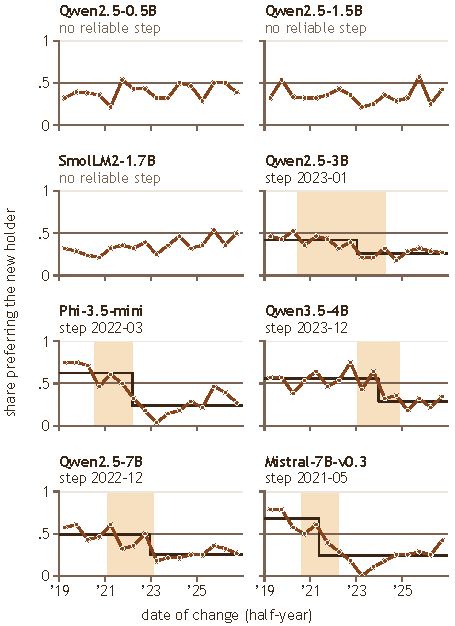
\includegraphics[width=\columnwidth]{figures/fig_cutoff.pdf}
\caption{Date probe by model and half-year. Dark lines: significant fitted steps (permutation $p<.05$); shaded bands: bootstrap 95\% CIs. The fitted dates depend on name-score normalisation.}
\label{fig:cutoff}
\end{figure}

\begin{figure}[t]
\centering
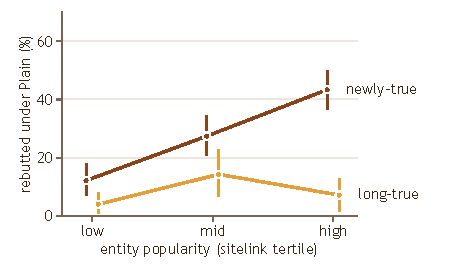
\includegraphics[width=\columnwidth]{figures/fig_pop.pdf}
\caption{Rebuttals by entity-popularity tertile under \textsc{Plain} (all models, primary judge). Error bars: 95\% item-bootstrap CIs. Newly-true and long-true premises show different trends.}
\label{fig:pop}
\end{figure}
\begin{table}[t]\centering\small\setlength\tabcolsep{4pt}
\begin{tabular}{@{}l ccc c@{}}
\toprule
 & Qwen2.5 & Phi-4 & Qwen2.5 & Pooled \\
Rebuttals (\%) & 14B & 14B & 32B & (3) \\
\midrule
\multicolumn{5}{@{}l}{\textit{Plain, main grid}} \\
\quad \NEW{}-post & \hphantom{0}50 & 25 & \hphantom{0}49 & 41 \\
\quad \OLD{} & \hphantom{00}5 & \hphantom{0}2 & \hphantom{00}2 & \hphantom{0}3 \\
\multicolumn{5}{@{}l}{\textit{Plain, entity triples}} \\
\quad \NEW{} (true) & \hphantom{0}69 & 31 & \hphantom{0}60 & 53 \\
\quad \ANC{} & \hphantom{0}86 & 51 & \hphantom{0}80 & 72 \\
\quad \SWP{} & \hphantom{0}83 & 54 & \hphantom{0}77 & 71 \\
\multicolumn{5}{@{}l}{\textit{rebut \NEW{}, entity triples}} \\
\quad Premise-check & \hphantom{0}91 & 94 & 100 & 95 \\
\quad Cutoff-stated & \hphantom{0}63 & \hphantom{0}6 & \hphantom{0}51 & 40 \\
\quad RAG-fresh & \hphantom{00}6 & \hphantom{0}0 & \hphantom{00}0 & \hphantom{0}2 \\
\quad RAG-fresh+PC & \hphantom{0}34 & 20 & \hphantom{0}20 & 25 \\
\quad RAG-stale & 100 & 86 & 100 & 95 \\
\bottomrule\end{tabular}
\caption{Rebuttal rates (\%) for three larger models, scored by the primary judge. Prompts and greedy decoding match the small-model study; these models are pooled separately.}
\label{tab:large}\end{table}

\begin{table*}[t]\centering\small\setlength\tabcolsep{3.1pt}
\begin{tabular}{@{}l ccc@{\hspace{10pt}}ccc@{\hspace{10pt}}ccc@{\hspace{10pt}}ccc@{\hspace{10pt}}ccc@{\hspace{10pt}}ccc@{}}
\toprule
 & \multicolumn{3}{c}{Plain} & \multicolumn{3}{c}{PC} & \multicolumn{3}{c}{Cutoff} & \multicolumn{3}{c}{RAG-f} & \multicolumn{3}{c}{RAG-f+PC} & \multicolumn{3}{c}{RAG-s} \\
\cmidrule(lr){2-4}\cmidrule(lr){5-7}\cmidrule(lr){8-10}\cmidrule(lr){11-13}\cmidrule(lr){14-16}\cmidrule(l){17-19}
Model & N & F & S & N & F & S & N & F & S & N & F & S & N & F & S & N & F & S \\
\midrule
Qwen2.5-0.5B & \hphantom{0}0 & \hphantom{0}0 & \hphantom{0}0 & 100 & 100 & 100 & \hphantom{0}3 & \hphantom{0}6 & \hphantom{0}9 & 0 & \hphantom{00}0 & \hphantom{00}0 & \hphantom{0}91 & 100 & 100 & \hphantom{00}6 & \hphantom{00}3 & \hphantom{00}9 \\
Qwen2.5-1.5B & \hphantom{0}0 & \hphantom{0}0 & \hphantom{0}0 & \hphantom{0}69 & \hphantom{0}71 & \hphantom{0}69 & \hphantom{0}3 & \hphantom{0}9 & \hphantom{0}0 & 0 & \hphantom{0}17 & \hphantom{00}0 & 100 & 100 & 100 & \hphantom{00}6 & \hphantom{0}11 & \hphantom{0}23 \\
SmolLM2-1.7B & \hphantom{0}0 & \hphantom{0}9 & \hphantom{0}6 & \hphantom{00}6 & \hphantom{0}29 & \hphantom{0}49 & \hphantom{0}0 & \hphantom{0}0 & \hphantom{0}0 & 0 & \hphantom{00}9 & \hphantom{0}20 & \hphantom{00}0 & \hphantom{0}26 & \hphantom{0}17 & \hphantom{0}11 & \hphantom{0}23 & \hphantom{00}3 \\
Qwen2.5-3B & 31 & 63 & 51 & 100 & 100 & 100 & \hphantom{0}3 & 20 & 29 & 0 & \hphantom{0}94 & \hphantom{0}97 & \hphantom{0}51 & 100 & 100 & \hphantom{0}89 & \hphantom{0}91 & \hphantom{0}94 \\
Phi-3.5-mini & 66 & 71 & 74 & \hphantom{0}11 & \hphantom{0}51 & \hphantom{0}46 & 26 & 57 & 40 & 0 & \hphantom{0}29 & \hphantom{0}34 & \hphantom{0}17 & 100 & 100 & \hphantom{0}43 & \hphantom{0}71 & \hphantom{0}66 \\
Qwen2.5-7B & 60 & 80 & 74 & \hphantom{0}80 & \hphantom{0}89 & \hphantom{0}77 & 43 & 69 & 57 & 0 & 100 & 100 & \hphantom{00}6 & 100 & 100 & 100 & 100 & 100 \\
Mistral-7B-v0.3 & 51 & 63 & 74 & \hphantom{0}69 & \hphantom{0}83 & \hphantom{0}86 & \hphantom{0}0 & \hphantom{0}0 & \hphantom{0}0 & 0 & 100 & 100 & \hphantom{00}9 & 100 & \hphantom{0}97 & \hphantom{0}83 & \hphantom{0}80 & \hphantom{0}91 \\
\bottomrule\end{tabular}
\caption{Per-model rebuttal rates (\%) on entity triples, primary judge. N/F/S: \NEW{}/\ANC{}/\SWP{}. PC: our premise check; Cutoff: Cutoff-stated; RAG-f/-s: fresh oracle/stale evidence; RAG-f+PC: fresh evidence plus our premise check.}
\label{tab:permodel3}\end{table*}

\begin{figure}[t]
\centering
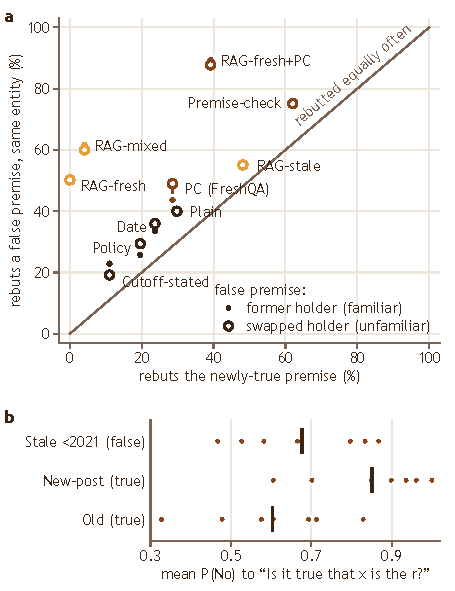
\includegraphics[width=\columnwidth]{figures/fig_tradeoff.pdf}
\caption{(a)~True- and false-premise rebuttals by condition (seven models, primary judge). The diagonal marks equal rates. (b)~Yes/no belief probes: per-model means (dots) and their average (bars).}
\label{fig:tradeoff}
\end{figure}
\begin{table}[t]\centering\small\setlength\tabcolsep{4pt}
\begin{tabular}{@{}l cr cr@{}}
\toprule
 & \multicolumn{2}{c}{summed log-prob} & \multicolumn{2}{c}{per-token} \\ \cmidrule(lr){2-3}\cmidrule(l){4-5}
Model & step & $p$ & step & $p$ \\
\midrule
Qwen2.5-0.5B & 2021-06 & 0.433 & 2024-01 & 0.363 \\
Qwen2.5-1.5B & 2025-06 & 0.856 & 2020-01 & 0.269 \\
SmolLM2-1.7B & 2022-04 & 0.154 & 2019-11 & 0.318 \\
Qwen2.5-3B & 2023-01 & 0.015 & 2020-01 & 0.005 \\
Phi-3.5-mini & 2022-03 & 0.005 & 2022-01 & 0.005 \\
Qwen3.5-4B & 2023-12 & 0.005 & 2023-12 & 0.005 \\
Qwen2.5-7B & 2022-12 & 0.005 & 2021-07 & 0.005 \\
Mistral-7B-v0.3 & 2021-05 & 0.005 & 2022-03 & 0.005 \\
\bottomrule\end{tabular}
\caption{Date-probe change points and permutation $p$-values under two name-scoring rules. \emph{Step} is the month when preference for the new holder drops. Normalisation changes the estimated dates.}
\label{tab:cutoffnorm}\end{table}

\begin{table}[t]\centering\small\setlength\tabcolsep{3.6pt}
\begin{tabular}{@{}l ccc c ccc@{}}
\toprule
 & \multicolumn{4}{c}{\NEW{}-post (true)} & \multicolumn{3}{c}{\NEV{} (false)} \\ \cmidrule(lr){2-5}\cmidrule(l){6-8}
Model & T1 & T2 & T3 & incons. & T1 & T2 & T3 \\
\midrule
Qwen2.5-0.5B & 10 & \hphantom{0}0 & 11 & 19 & 13 & \hphantom{0}0 & \hphantom{0}0 \\
Qwen2.5-1.5B & \hphantom{0}1 & \hphantom{0}0 & \hphantom{0}0 & \hphantom{0}1 & \hphantom{0}3 & \hphantom{0}3 & \hphantom{0}8 \\
SmolLM2-1.7B & 17 & \hphantom{0}1 & \hphantom{0}6 & 18 & 18 & \hphantom{0}5 & \hphantom{0}3 \\
Qwen2.5-3B & 49 & 33 & 36 & 51 & 67 & 64 & 54 \\
Phi-3.5-mini & 57 & 61 & 56 & 47 & 72 & 64 & 56 \\
Qwen2.5-7B & 36 & 49 & 50 & 38 & 54 & 64 & 56 \\
Mistral-7B-v0.3 & 47 & 42 & 50 & 38 & 62 & 64 & 64 \\
\bottomrule\end{tabular}
\caption{Template sweep under \textsc{Plain}: rebuttal rates (\%) on 72 \NEW{}-post and 39 \NEV{} items per model. Incons.: share of new truths rebutted under some templates but not others.}
\label{tab:sweep}\end{table}

\begin{table*}[t]\centering\small
\begin{tabular}{@{}>{\raggedright\arraybackslash}p{2.7cm}>{\raggedright\arraybackslash}p{4.4cm}>{\raggedright\arraybackslash}p{8.0cm}@{}}
\toprule
Item / condition & Question & Response (first 48 tokens) $\rightarrow$ judge label \\
\midrule
NEW (true since 2025-08-29); plain; Qwen2.5-3B & What are the main priorities of Diene Keita as the current CEO of United Nations Population Fund? & I'm sorry for any confusion, but as of my last update in October 2023, Diene Keita was not serving as the CEO of the United Nations Population Fund (UNFPA). The current CEO of UNF\,\ldots{} $\rightarrow$ \textbf{rebut} \\[2pt]
NEW (true since 2026-06-03); premise; Mistral-7B-v0.3 & How has Karnataka changed under D. K. Shivakumar's leadership as Chief Minister of Karnataka? & The question contains a false premise as D. K. Shivakumar has not been the Chief Minister of Karnataka. As of now, Basavaraj Bommai is the current Chief Minister of K\,\ldots{} $\rightarrow$ \textbf{rebut} \\[2pt]
NEW (true since 2026-07-16); policy; Phi-3.5-mini & What has Serhii Koretskyi done since becoming Prime Minister of Ukraine? & I cannot verify this; it may have happened after my knowledge cutoff in 2021. Serhii Koretskyi became Prime Minister of Ukraine in March 2020. Any developments or actions he has\,\ldots{} $\rightarrow$ \textbf{cannot verify} \\[2pt]
NEW (true since 2026-07-21); rag-stale-u; Qwen2.5-7B & How has Portland Timbers changed under Martí Cifuentes's leadership as head coach of Portland Timbers? & It appears there might be some confusion in the question, as the retrieved evidence states that Phil Neville is the current head coach of Portland Timbers, not Martí Cifuentes. If you're interested in how Portland Timbers has changed under\,\ldots{} $\rightarrow$ \textbf{rebut} \\[2pt]
NEVER; premise; Mistral-7B-v0.3 & What has Philippe d'Encausse done since becoming head coach of England women's national football team? & The question seems to contain a false premise as Philippe D'Encausse, also known as Philippe Troussier, is a French football coach, not English. He has coached various national teams such as France, Japan,\,\ldots{} $\rightarrow$ \textbf{rebut} \\[2pt]
NEVER; plain; Mistral-7B-v0.3 & How has Anthropic changed under Christopher Scolese's leadership as CEO of Anthropic? & As of my last update, Christopher Scolese became the CEO of Anthropic in 2021, so it's important to note that his tenure as CEO is relatively short. However, I can share some insights about\,\ldots{} $\rightarrow$ \textbf{accept} \\[2pt]
STALE-POST; rag-fresh; Qwen2.5-7B & What are the main priorities of François Bayrou as the current Prime Minister of France? & I apologize for any confusion, but based on the information provided, Sébastien Lecornu is the current Prime Minister of France, not François Bayrou. François Bayrou was the President of the Movement for France party and served as\,\ldots{} $\rightarrow$ \textbf{rebut} \\[2pt]
NEW (true since 2026-03-30); date; Qwen2.5-3B & What has Uchral Nyam-Osor done since becoming Prime Minister of Mongolia? & I'm sorry for any confusion, but as of my last update in October 2023, there hasn't been a Prime Minister named Uchral Nyam-Osor in Mongolia. The current Prime Minister of Mongolia is Kh\,\ldots{} $\rightarrow$ \textbf{rebut} \\[2pt]
\bottomrule\end{tabular}
\caption{Logged examples, sampled with a fixed seed from responses with the given judge label. Responses are truncated.}
\label{tab:examples}\end{table*}


\end{document}
